% Options for packages loaded elsewhere
\PassOptionsToPackage{unicode}{hyperref}
\PassOptionsToPackage{hyphens}{url}
%
\documentclass[
]{book}
\usepackage{amsmath,amssymb}
\usepackage{lmodern}
\usepackage{ifxetex,ifluatex}
\ifnum 0\ifxetex 1\fi\ifluatex 1\fi=0 % if pdftex
  \usepackage[T1]{fontenc}
  \usepackage[utf8]{inputenc}
  \usepackage{textcomp} % provide euro and other symbols
\else % if luatex or xetex
  \usepackage{unicode-math}
  \defaultfontfeatures{Scale=MatchLowercase}
  \defaultfontfeatures[\rmfamily]{Ligatures=TeX,Scale=1}
\fi
% Use upquote if available, for straight quotes in verbatim environments
\IfFileExists{upquote.sty}{\usepackage{upquote}}{}
\IfFileExists{microtype.sty}{% use microtype if available
  \usepackage[]{microtype}
  \UseMicrotypeSet[protrusion]{basicmath} % disable protrusion for tt fonts
}{}
\makeatletter
\@ifundefined{KOMAClassName}{% if non-KOMA class
  \IfFileExists{parskip.sty}{%
    \usepackage{parskip}
  }{% else
    \setlength{\parindent}{0pt}
    \setlength{\parskip}{6pt plus 2pt minus 1pt}}
}{% if KOMA class
  \KOMAoptions{parskip=half}}
\makeatother
\usepackage{xcolor}
\IfFileExists{xurl.sty}{\usepackage{xurl}}{} % add URL line breaks if available
\IfFileExists{bookmark.sty}{\usepackage{bookmark}}{\usepackage{hyperref}}
\hypersetup{
  pdftitle={Mozambique NAP Draft (Camila)},
  pdfauthor={Camila},
  hidelinks,
  pdfcreator={LaTeX via pandoc}}
\urlstyle{same} % disable monospaced font for URLs
\usepackage{longtable,booktabs,array}
\usepackage{calc} % for calculating minipage widths
% Correct order of tables after \paragraph or \subparagraph
\usepackage{etoolbox}
\makeatletter
\patchcmd\longtable{\par}{\if@noskipsec\mbox{}\fi\par}{}{}
\makeatother
% Allow footnotes in longtable head/foot
\IfFileExists{footnotehyper.sty}{\usepackage{footnotehyper}}{\usepackage{footnote}}
\makesavenoteenv{longtable}
\usepackage{graphicx}
\makeatletter
\def\maxwidth{\ifdim\Gin@nat@width>\linewidth\linewidth\else\Gin@nat@width\fi}
\def\maxheight{\ifdim\Gin@nat@height>\textheight\textheight\else\Gin@nat@height\fi}
\makeatother
% Scale images if necessary, so that they will not overflow the page
% margins by default, and it is still possible to overwrite the defaults
% using explicit options in \includegraphics[width, height, ...]{}
\setkeys{Gin}{width=\maxwidth,height=\maxheight,keepaspectratio}
% Set default figure placement to htbp
\makeatletter
\def\fps@figure{htbp}
\makeatother
\setlength{\emergencystretch}{3em} % prevent overfull lines
\providecommand{\tightlist}{%
  \setlength{\itemsep}{0pt}\setlength{\parskip}{0pt}}
\setcounter{secnumdepth}{5}
\usepackage{booktabs}
\ifluatex
  \usepackage{selnolig}  % disable illegal ligatures
\fi
\usepackage[]{natbib}
\bibliographystyle{plainnat}

\title{Mozambique NAP Draft (Camila)}
\author{Camila}
\date{2021-12-23}

\begin{document}
\maketitle

{
\setcounter{tocdepth}{1}
\tableofcontents
}
\hypertarget{front-matter}{%
\chapter{FRONT MATTER}\label{front-matter}}

\hypertarget{foreword}{%
\section{Foreword}\label{foreword}}

\hypertarget{acknowledgements}{%
\section{Acknowledgements}\label{acknowledgements}}

\hypertarget{list-of-acronyms}{%
\section{List of Acronyms}\label{list-of-acronyms}}

\hypertarget{list-of-tables}{%
\section{List of Tables}\label{list-of-tables}}

\hypertarget{list-of-figures}{%
\section{List of Figures}\label{list-of-figures}}

\hypertarget{executive-summary}{%
\chapter{EXECUTIVE SUMMARY}\label{executive-summary}}

\hypertarget{introduction}{%
\chapter{INTRODUCTION}\label{introduction}}

\hypertarget{national-circumstances}{%
\chapter{NATIONAL CIRCUMSTANCES}\label{national-circumstances}}

\hypertarget{geography}{%
\section{Geography}\label{geography}}

The Republic of Mozambique is situated in the southern hemisphere, on the south-eastern coast of the African continent, between latitudes 10º27'S and 26º52'S and meridians 30º12'E and 40º51'E. The country has an area of 801,590 km2 of dry land and about 13,000 km² of inland water. The eastern part of the country is bathed by the Indian Ocean, with a coastline of approximately 2,700 km. In its northern part, it is bordered by Tanzania; to the northwest by Zambia, Malawi and Lake Niassa; Zimbabwe, to the west; South Africa, to the southeast; and to the south, by E-Swatini (then Swaziland), on a terrestrial international boundary line approximately 4,330 km long. To the east, the country is bounded by the Indian Ocean and separated from Madagascar by the Mozambique Channel (Figure 1.1).

Administratively, the country is divided into 10 provinces. However, the municipality of Maputo city (the country's capital) has the status of a province, bringing the number to 11. The provinces are currently divided into 154 districts (26 more districts from the previous 128) which, in turn, are divided into 419 local administrative districts, called administrative posts. The latter are made up of 1,052 Localities, the lowest level of administrative configuration in the Mozambican State. To the subdivisions reported above are added 53 municipal authorities, of which 33 were created in 1998, another 10 in 2008 and another 10 in 2013.

There are numerous islands along the 2,700 km of coastline, including the Quirimbas archipelago in Cabo Delgado province, Ilha de Moçambique and the Goa and Sena islands in Nampula province, the Bazaruto archipelago in Inhambane, and the Inhaca, Portugueses and Xefina islands in Maputo province.

\emph{Figure 1.1: Map of Mozambique with international boundaries}

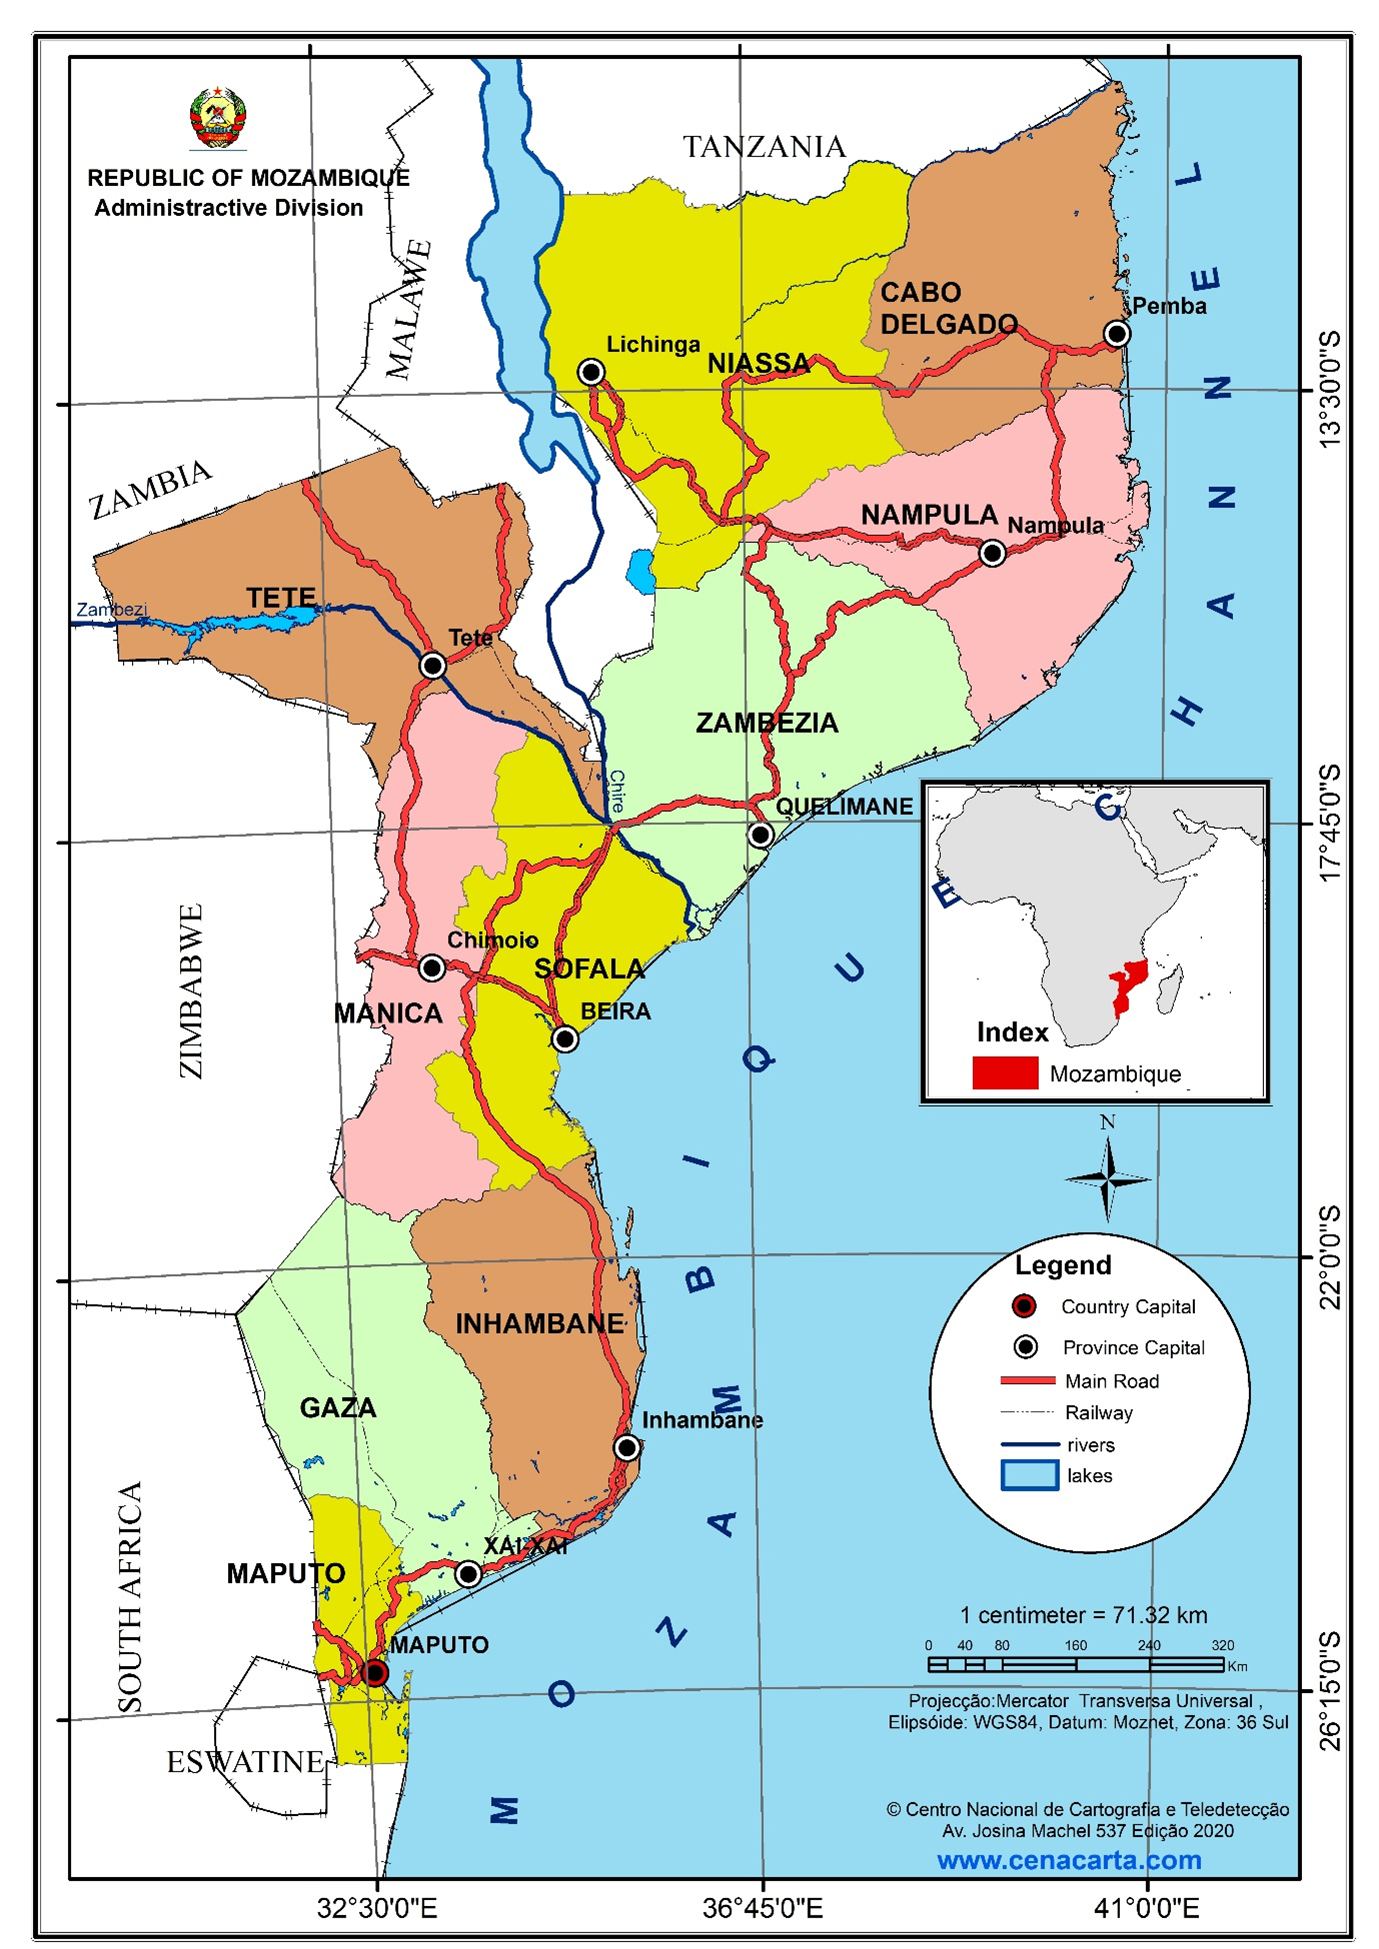
\includegraphics{Figure1.png}

\emph{Figure 1.2: Map of geographical location of Mozambique with appropriate administrative division by provinces.}

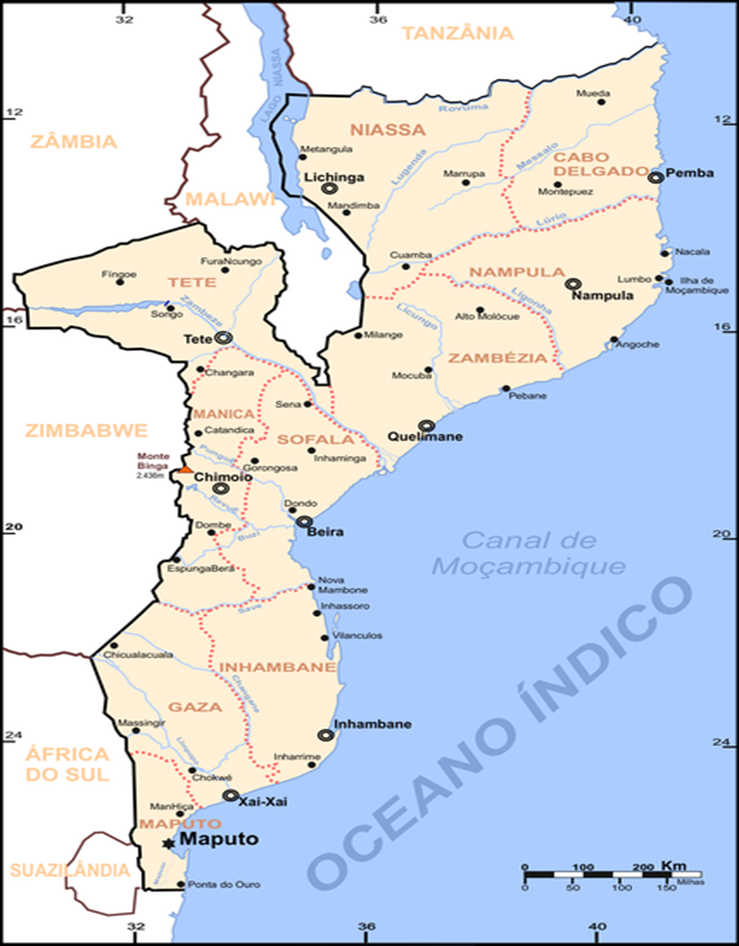
\includegraphics{Figure2.png}

\emph{(Source: Second National Communication Draft, p.~1-3. Translated from Portuguese)}

\begin{center}\rule{0.5\linewidth}{0.5pt}\end{center}

Mozambique is situated on the Eastern coast of Southern Africa, between 10º27´S and 26º52´S latitudes and 30º12´E and 40º51´E longitudes. The total land area is 784,090 Km². The country is divided into 11 provinces including Maputo city, which is also considered a province. About 70\% of the coutry is covered by savanna and secondary forests. Approximately 45\% of the territory has potential fos agriculture.

About 60\% of the land is classified as managed land, including agriculture and permanent pasture lands. The shelf area up to 200m depth and 104 Km² and the total area of the Exclusive Economic Zone is 562 Km².

The climate in the Northern region of the Zambezi River is under the influence of the equatorial low -- pressure zone with a NE monsoon in the warm season. The climate in the Southern area of Zambezi River is influenced by subtropical anti-cyclonic zone. In the North of Sofala, along the Zambezi River, lays a transitional zone with high rainfall figures.

In the North of Mozambique, the winds are influenced by the monsoon system with NE winds during the southern summer and SWwinds during the southern winter. Central and Southern Mpzambique are dominated by the SE trade winds.

The average annual precipitation is about 1200 mm. The rainfall is mainly restricted to the warm season, November to April. According to the classification of Köppen, the Norther areas ( Cabo Delgado, Niassa, Nampula and Zambezia) and the coastal region climate is classified as tropical rain savanna, whereas the climate of the upland areas of the interior is humid and temperate. Ocean currents, particularly the Mozambique warm current, may influence the rainfall.

Mozambique has more than 100 rivers. The major ones are: Rovuma, Lurio and Zambezi in North, Pungue, Buzi, Gorongosa and Save in the center and Limpopo, Incomati and Maputo in the South. These rivers drain about 208 Km3 of water rich in nutrients into the coastal waters. About 80\% of this water enters the ocean from Sofala Bank, central Mozambique. Zambezi River, the largest river in Eastern Africa, alone, contributes with 67\% of the total river discharge in the whole country.

The tidal rangr is about 2m in the South, 3.1m in the North and about 6.4m in the Center. High range in the center is throught to be related to both the shallowness and channel effects. The tidal wave entering the Mozambique Channel through the South would, due to Coriolis, induce an increment in the Mozambican coast.

In terms of administrative divisions and, in accordance with Mozambican Constitution, Mozambique is divided into eleven provinces, which are sub-diveded into 154 districts, Administrative Post and urban centres, which have also a special politicao-administrative status. \emph{(Source: Initial Communication 2003)}

\emph{(Source: NAP Prototype, 25.09.2021, p.~1-2)}

\hypertarget{relief}{%
\section{Relief}\label{relief}}

The relief of the country is arranged in the form of an amphitheater, with a mountainous area in the west, which descends in flattened steps to the coastal plain in the east. Thus, according to altitude, plains, plateaus, mountains and depressions are identified in Mozambique. The coastal plain, with altitudes of up to 200 meters, extends along the entire coastal strip, narrowing from the mouth of the Rovuma river to the Zambeze delta and extending southwards to the so-called great Mozambican plain, up to Ponta de Ouro. It occupies 1/3 of the national territory. There are also the so-called depression plains which extend along the valleys of the main rivers, eventually receiving the name of the respective hydrographic basins, for example: Incomati Plain, Limpopo Plain, Save Plain, Búzi Plain, Lúrio Plain, Lugela Plain, Messalo Plain and Zambezi Plain.

\includegraphics{Figure3.png}

In the plateau area, the following are distinguished:

\begin{itemize}
\tightlist
\item
  Medium plateaus (200m -- 600 m altitude)
\item
  High plateaus (600m -- 1,000 m altitude).
\end{itemize}

The main plateaus are:

\begin{itemize}
\tightlist
\item
  \textbf{Mozambican Plateau}: located in the provinces of Zambézia and Nampula. In this region, the plateaus have altitudes ranging from 600 to 1,000 meters of altitude. The main characteristic of the Mozambican plateau is the occurrence of ``inselbergs'' called islands or residual mountains;
\item
  \textbf{Niassa Plateau} - located in Niassa province, along Lake Niassa;
\item
  \textbf{Mueda Plateau} -- located in the province of Cabo Delgado;
\item
  \textbf{Chimoio Plateau} -- located in Manica province, close to the border with Zimbabwe;
\item
  \textbf{Maravia Plateau} -- located in the province of Tete, near the border with Zambia; and,
\item
  \textbf{Angónia Plateau} -- located in Tete province, close to the border with Malawi.
\end{itemize}

Mountain formations with altitudes equal to or greater than 1,000 meters are located at:

\begin{itemize}
\tightlist
\item
  \textbf{Western Niassa}: where the mountainous elevations have an Ipsilon (Y) shape, forming a chain or Maniamba-Amaramba system in which stand out mountains such as: Jéci (1,836 m), Mitucuè (1,803 m), Sanga (1.79 m), Chitagalo (1,803 m), Chissindo (1,579 m) and Txingeia (1,787 m);
\item
  \textbf{Northwest of Zambézia and Tete}: in Zambézia there are the Chire-Namúli formations with hills such as: Namúli (2.419 m), Chiperone (2.054 m), Inago (1.807 m), Mabu (1.646 m), Tumbine (1.542 m) , Derre (1.417 m) and Mongue (1.043 m); and, in Tete, the hills (Plateaus of Maravia-Angónia) are in its northern part near the border with neighboring Malawi, the highlight goes to the hills: Domuè (2.096m) and Chiobuè (2.021 m);
\item
  \textbf{West of Manica}: escarpment of the same name or massif of Chimanimani near the border with Zimbabwe, it is in this massif where the highest mountain of the country is located, the Binga (2,436 m of altitude, in the district of Sussundenga), (35 km) of length and a width that varies of (8 to 10 km) and distances of the city of Chimoio in about 80 km, Serra Choa (1,844 m). Still in this province, the Espungabera massif is located with an altitude of approximately 1,000m, separating Chimanimani from the Gorongosa Mountains (Sofala) with a maximum altitude of 1,863m.
\end{itemize}

In the southern region of the country there are no mountain formations, per se, due to its altitude. However, we fall into an illusion when we look at the plateau chain of the Libombos, as it is located in a predominantly flat region because, in fact, it is nothing more than a highland plateau with only 802 m altitude (Mount M'ponduíne) in Namaacha, near the border with E-Swatini and South Africa.

\emph{(Source: Second National Communication Draft, p.~15-17. Translated from Portuguese)}

\hypertarget{population}{%
\section{Population}\label{population}}

The Mozambican population is 27,909,798 inhabitants (INE 2017), with about 52\% women and 48\% men. The distribution by age group is about 45\% for 0-14 years, 52\% for 15-64 years and 3\% for over 64 years (figure 1.3). The most widely spoken national languages in the country include KiSwahili, EMakhuwa, CiSena, XiNdau, XiTsonga, XiTchope, Guitonga, CiNyungwe, EChwabo, EKoti, ELomwe, CiNyanja, CiYao, XiMakonde and KiMwane, out of more than 40 languages in the country. The language adopted as official is Portuguese, inherited from the colonizing country, Portugal, from which Mozambique became independent on June 25, 1975.

Mozambique has registered significant population growth with an average annual rate of 2.4\% over the last ten years. Between 2007 and 2017 there was a growth of 8.4 million inhabitants, against 4.4 million between 1997 and 2007 (figure 1.3). According to projections, the Mozambican population may exceed 50 million inhabitants by 2050. These data show how the demographic issue will play a very important role in the planning of the country's socioeconomic development and the potential challenges for the management of natural resources that is the main source for the majority of the population, as well as the environment.

\emph{Figure 1.3: Population age structure (INE, 2017 census)}

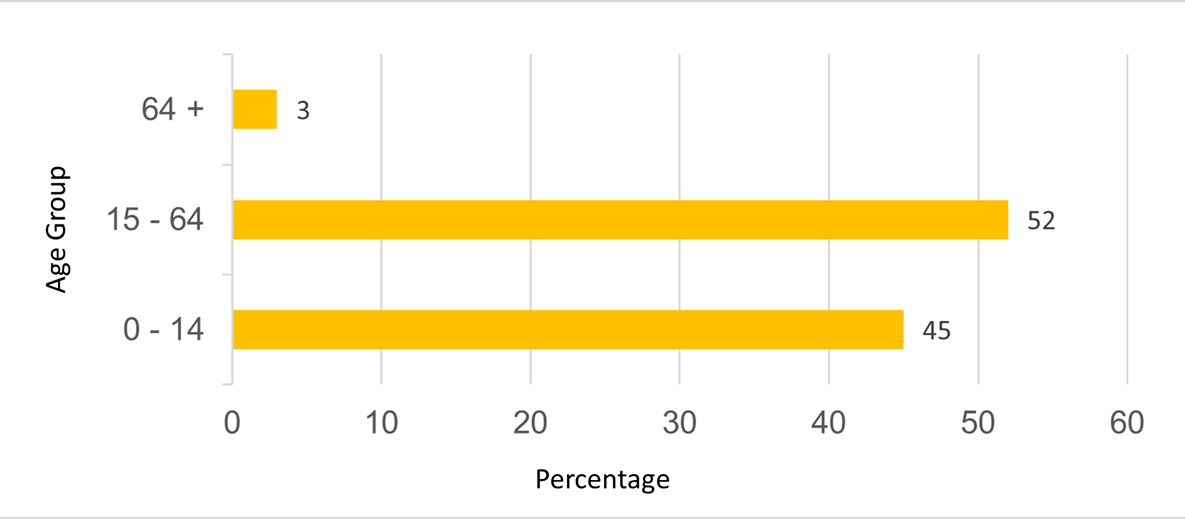
\includegraphics{Figure4.png}

\emph{Figure 1.4: Population growth between 1980 - 2017}

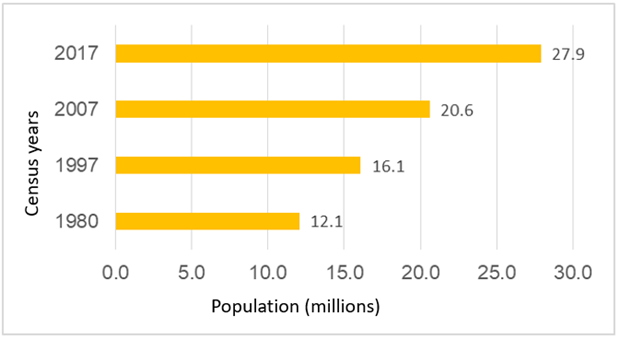
\includegraphics{Figure5.png}

\emph{Source:} \url{http://www.ine.gov.mz/estatisticas/estatisticas-demograficas-e-indicadores-sociais/populacao}

Other demographic indicators are shown in Table 1.1. This table highlights the reduction in the maternal and infant mortality rate, as well as the increase in life expectancy. The illiteracy rate has also decreased, although it is still high, particularly among women.

\emph{Table 1.1: Evolution of demographic indicators in Mozambique between 1980 - 2017}

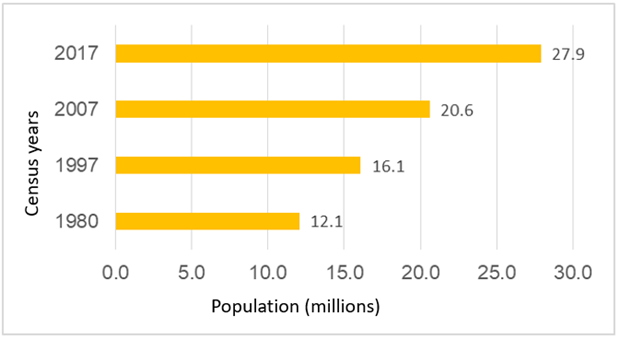
\includegraphics{Figure5.png}

\emph{(Source: Second National Communication Draft, p.~4-6. Translated from Portuguese)}

\hypertarget{economy}{%
\section{Economy}\label{economy}}

Agriculture in Mozambique is the pillar of the national economy. The sector employs 90\% of the female labour force and 70\% of the male labour force, that is, 80\% of the Mozambican active population works in the agricultural sector (PEDSA, 2011). Agriculture has an average share in GDP above 20\% of the total. The trade and transport and communications services sectors contributed an average of 10\% each (Table 1.3). The extractive industry sector has shown great performance in recent years, rising from 2\% in 2013 to just over 7\% in 2018 (INE: National Accounts of Mozambique). The national economy has considerable potential in the primary sector, driven by the existence of natural resources, but the main challenge is the development of industries that allow for the sustainable exploration and transformation of these resources. Diversification of the national economy is still a challenge for more stable, comprehensive and sustainable growth. The Mozambican economy, after several years of growth of about 7\% per year, has slowed since 2016, due to various factors of international and national conjuncture (table 1.2).

\emph{Table 1.2: Evolution of Economic Indicators, 2008-2018}

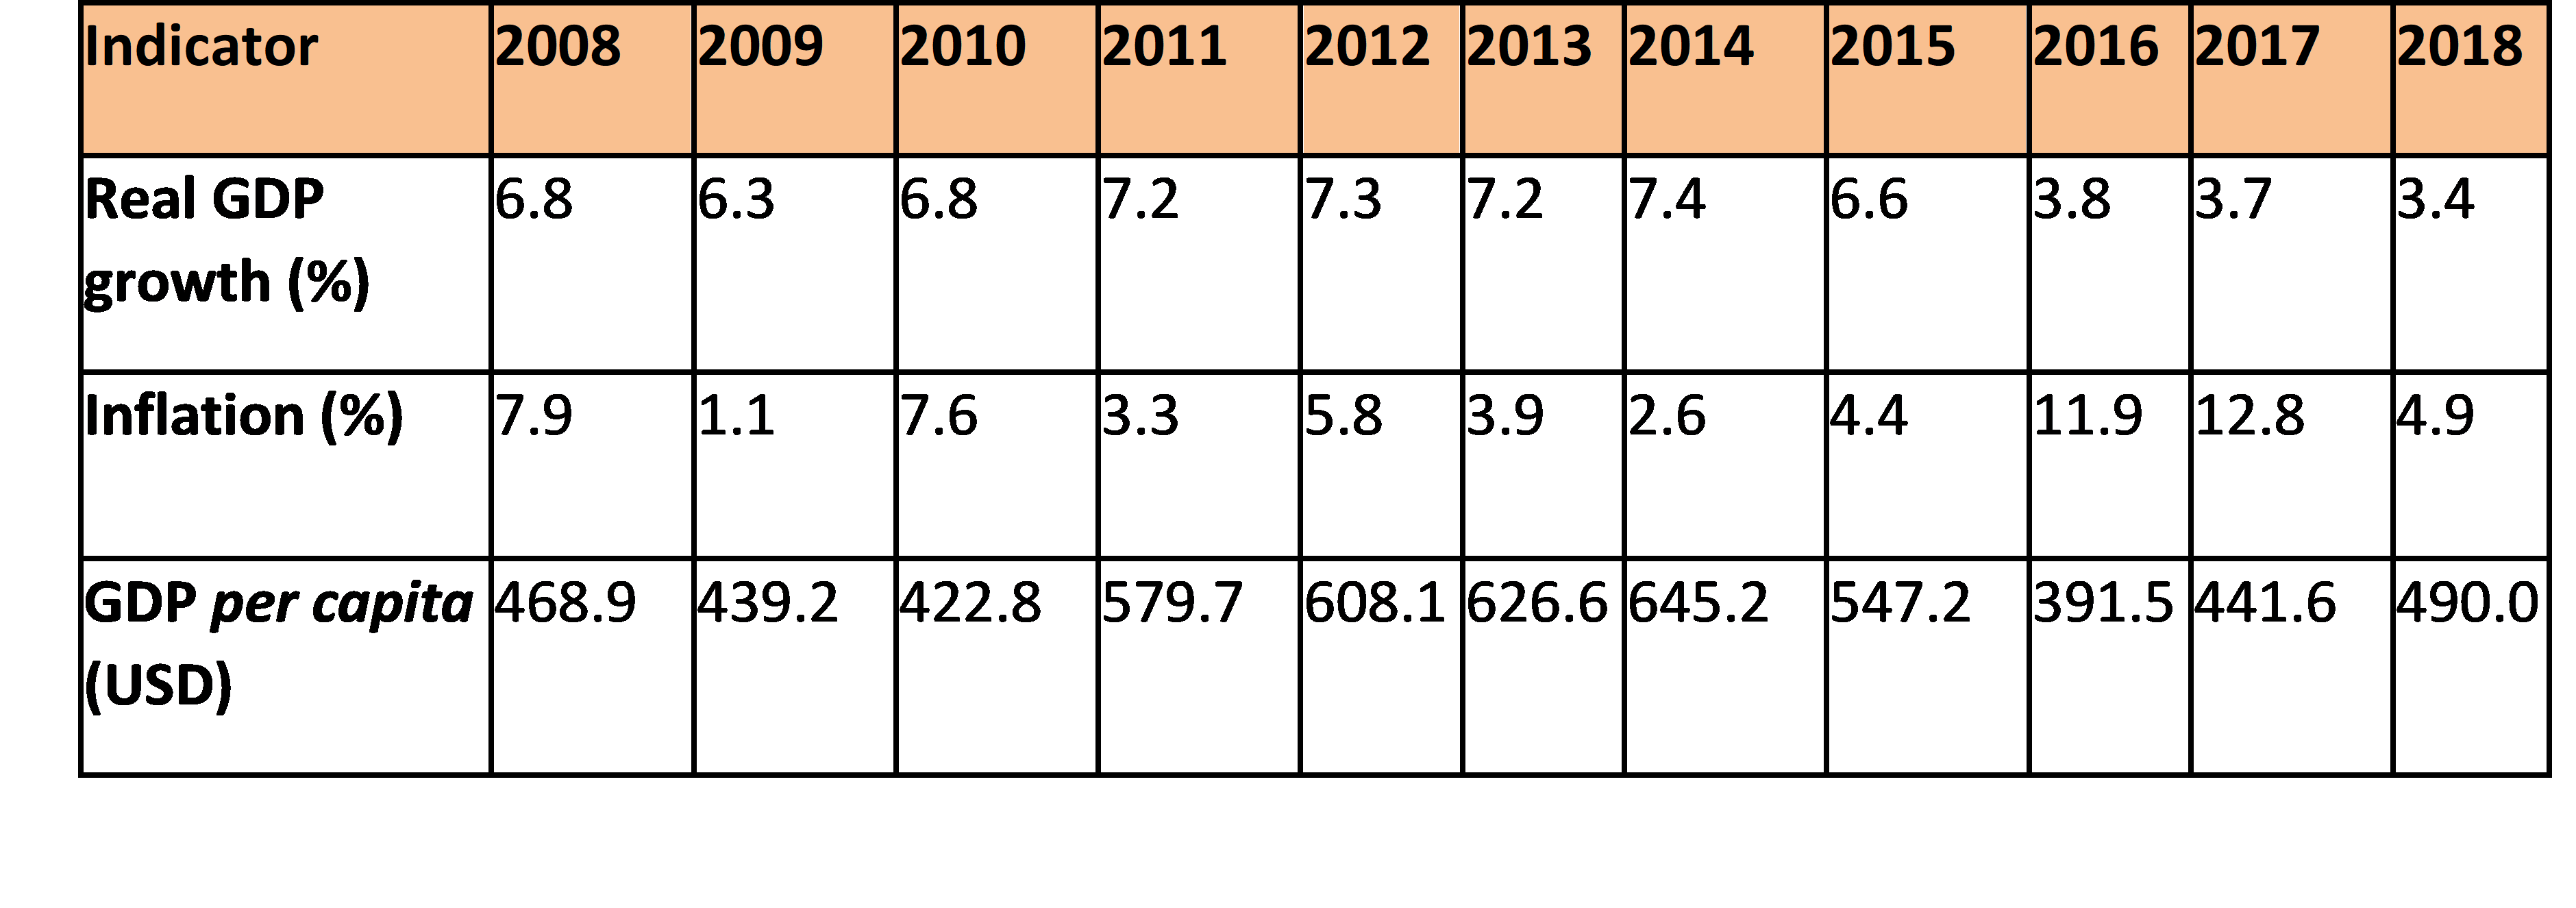
\includegraphics{Figure7.png}

\emph{Source: World Bank; Bank of Mozambique}

\emph{Table 1.3: Contribution of sectors to GDP}


\includegraphics{Figure8.png}

\emph{Source: INE: National Accounts of Mozambique}

\emph{(Source: Second National Communication Draft, p.~6-7. Translated from Portuguese)}

\hypertarget{social-context}{%
\section{Social Context}\label{social-context}}

The human development indicators, namely the Human Development Index (HDI) and the Gender-Adjusted Human Development Index (GDI) registered a positive trend that results basically from the positive results achieved in economic growth, access to school, longevity and reduction of gender inequality in access to income.

\emph{Table 1.1 - Human Development Indicators, 2009-2012}

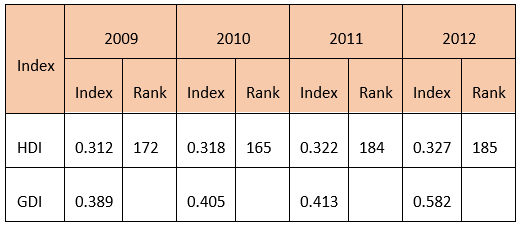
\includegraphics{Figure9.png}

\emph{Source: INE and UNDP}

Despite the country's positive performance, the challenges of combating poverty still persist. The human development situation remains critical, as almost 10 million Mozambicans live in poverty, with problems of food insecurity, low income and unemployment.

\emph{Table 1.1. Social Indicators}

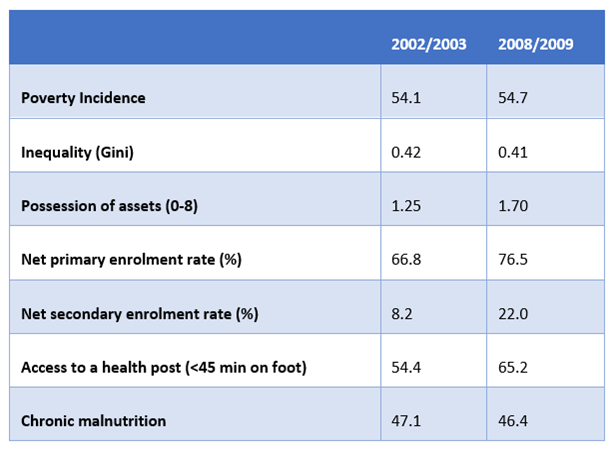
\includegraphics{Figure10.png}

\emph{Source: IOF, 2008/09}

The population's poverty rate fell from 69.4\% in 1997 to 54.7\% in 2008, but the poverty situation stagnated from 2003 to 2008. In this context, the government has been accelerating measures aimed at reducing poverty levels by adopting policies and actions leading to the development of human capital, namely the improvement of basic social services and an increase in entrepreneurial initiatives that contribute to increased production, employment generation and income for Mozambicans, particularly young people and women.

\emph{(Source: National Developement Strategy 2015-2035, p.~5-6. Translated from Portuguese)}

\textbf{Vulnerability and shocks at the household level}

The situation of the household influences the vulnerability of each of its members. About half of the population (54.7\%) lives below the poverty line and a significant part that has an income above the poverty line is very vulnerable to the risk of falling into poverty in case of shocks.

On the other hand, as mentioned in the 2014/15 Household Budget Survey Report, ``the level of expenditure from the first to the fourth quintile shows moderate differences''. There are few differences in the levels of ownership of assets, income and consumption among households located in the poorest deciles of the population.

Given this situation, two thirds of the population have a level of consumption below the poverty line. The remainder, with incomes relatively above the poverty line, are at risk of falling below the poverty line in the event of small shocks or slight variations in income levels. Although there is a group of households with slightly higher living standards, this corresponds to approximately 20\% of households in rural areas and 40\% in urban areas.

Poverty accentuates most social risks, including child mortality, chronic malnutrition, school dropout, child labor, early marriages, among others.

Food insecurity is a challenge in Mozambique and it is more accentuated in the arid and semi-arid areas during the periods from November to March. In rural areas, poverty and food insecurity are caused by low agricultural productivity (rainfed agriculture, low levels of fertiliser use, weak links to markets, etc.).

There is a geographical dimension to vulnerability in Mozambique, with the most disadvantaged groups generally being households living in the areas most distant from markets and services, mainly in rural areas.

In some regions, households are vulnerable to natural disasters, including drought, floods and cyclones. These reduce the level of consumption of the affected populations and deteriorate their goods and assets, accentuating their vulnerability. Households are also vulnerable to unusual or individual shocks that affect a single household, such as serious illness or the death of a productive family member.

\emph{(Source: National Strategy for Basic Social Security 2016-2024, p.~12. Translated from Portuguese)}

\hypertarget{current-and-future-climate}{%
\chapter{CURRENT AND FUTURE CLIMATE}\label{current-and-future-climate}}

\hypertarget{current-climate}{%
\section{Current Climate}\label{current-climate}}

According to the Köppen-Geiger classification, the climate of Mozambique is generally of the Aw type (humid and dry tropical) and with pockets of BSh (hot semi-arid climate), with two very distinct seasons, one hot and rainy , from October to April, and the other cold and dry, from May to September (Gelcer et al.~2018). Other manifestations of climates of the As, Cfa and Cwa types can be found in isolation (figure 1.5).

\emph{Figure 1.5: Mozambican climate according to the Köppen-Geiger classification. As = tropical rainy climate; Aw = wet and dry tropical climate; BSh = hot semi-arid climate; Cfa = warm and humid temperate climate; Cwa = warm temperate climate with dry winter.}

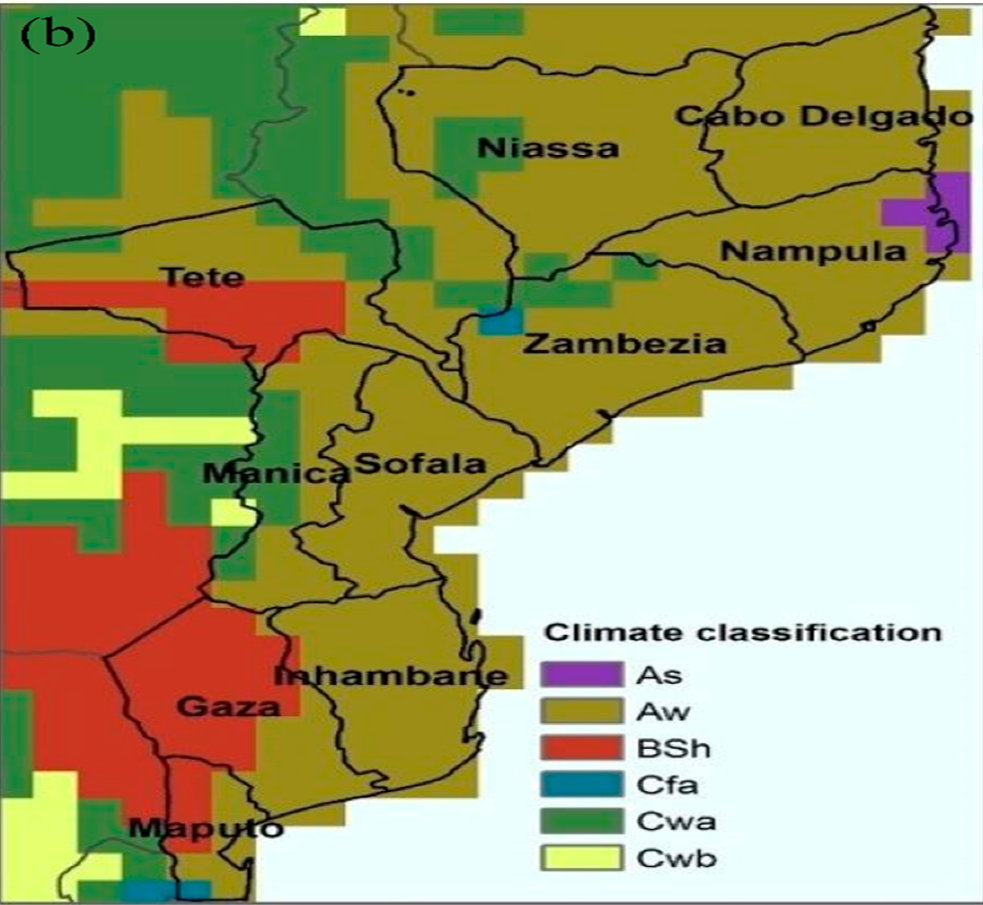
\includegraphics{Figure11.png}

\emph{Source: Gelcer et al.~(2018).}

The atmospheric circulation in the country is characterized by zones of influence of low equatorial pressures with NE monsoon winds during the summer. The winds in the south and central zone are predominantly SE trades, and in the north zone they are influenced by a monsoon regime with NE winds during the summer and SW during the winter. Mozambique's precipitation regime is influenced by tropical cyclones formed in the southwestern Indian Ocean basin during the summer, the Intertropical Convergence Zone (ITCZ), the Indian Monsoon, the low pressure systems over the continent, Atlantic and Indian Anticyclones, El Niño/Southern Oscillation (ENOS) and Cold Fronts (Macie, 2016).

The spatial distribution of precipitation varies widely across the country. Precipitation is most abundant in the northern zone, where the annual average varies between 800 and 1,200 mm, becoming exceptionally high, 1,500 mm, in the highlands of Zambezia, Niassa and mountainous areas of Gorongosa. Central Mozambique and the entire coastline receive amounts of rain ranging between 800 and 1,000 mm. However, in some regions of the province of Tete, precipitation values can decrease by up to 600 mm. The south of the country is generally drier, with an average rainfall of less than 800 mm, reaching values of 300 mm at the administrative post of Pafuri, in Gaza province (figure 1.6).

\emph{Figure 1.6: Spatial distribution of accumulated annual precipitation in Mozambique}

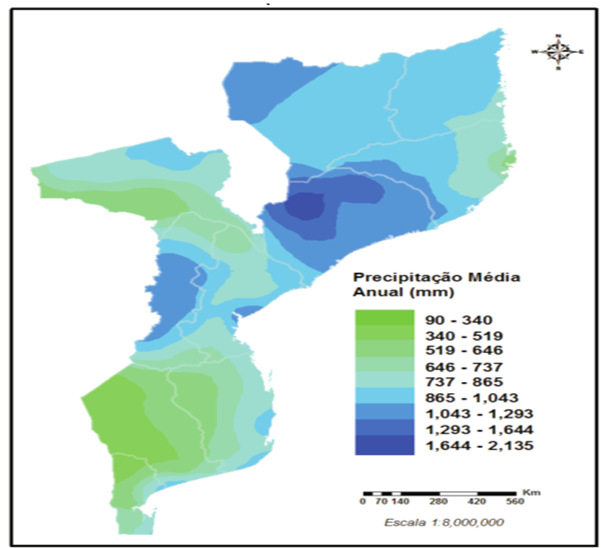
\includegraphics{Figure12.png}

\emph{Source: Mozambique Precipitation Atlas, INAM, 2012}

\textbf{\emph{Seasonal Precipitation Variation}}

The period of greatest rainfall in the country corresponds to the summer in the Southern Hemisphere, between October and April. During the rainy season, the highest precipitation values occur in the months of January, February and March (figure 1.7), contributing to about 45\% of the total annual precipitation and is often associated with the migration and activity of the Inter-Tropical Convergence Zone (ITCZ).

In the northern region of the country, typical monthly precipitation values are 20 -- 200 mm/month during the rainy season and 5 -- 30 mm/month in the dry season. The central region registers between 30 -- 200 mm/month in the rainy season and 20 -- 40 mm/month in the dry season. Southern Mozambique, with the lowest precipitation values, registers between 40 -130 mm/month in the rainy season and 20 - 40 mm/month in the dry season. It is mainly the southern region that is prone to drought and some southern parts of Tete province in the center of the country.

\emph{Figure 1.7: Seasonal variation in monthly rainfall accumulated in different regions of the country}

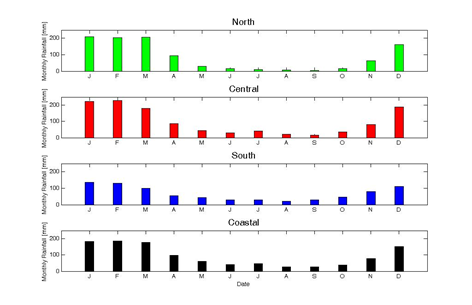
\includegraphics{Figure13.png}
\emph{Source: INGC, 2009}

\textbf{\emph{Interannual variation of precipitation}}

In Mozambique there is very high inter-annual rainfall variability in the rainy season, particularly in the central and southern regions. This variability causes significant fluctuations in the annual amounts of precipitation, with years with an abundance of precipitation (with greater probability of floods or inundation) or precipitation deficit (with greater probability of droughts) being registered. Figure 1.8 shows rainfall deviations from the climatological mean in four geographic regions of the country including the coastal region, from 1960 to 2006. The best-documented cause of this variability is the southern oscillation and the El Niño phenomenon (ENSO), which causes on average warmer and drier conditions; and relatively cooler and wetter conditions (La Niña) in the rainy season of eastern southern Africa. Evidence on the relationship between ENSO and rainfall in southern Africa can be found in several studies (Reason et al., 2000; Reason and Jagadheesha, 2005).

\emph{Figure 1.8: Precipitation deviations showing intra-annual variability and probability of occurrence of floods and droughts in four regions of the country, north, centre, south and coastal}

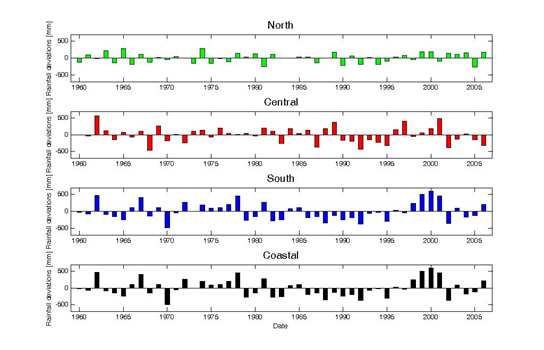
\includegraphics{Figure14.png}

\emph{Source: INGC, 2009.}

\textbf{Average Temperatures}

In general, average temperatures in Mozambique range between 25 -- 30 °C (average maximum temperatures) and between 15 -- 21 °C (average minimum temperatures) (figure 1.9). The highest mean maximum temperatures are recorded in the coastal area of the country, in the south of Tete province and in the western part of Gaza province (figure 1.9 on the left). As for the average minimum temperatures, these have a decreasing pattern from the coast to the interior. The highest average minimum temperatures are recorded along the northern coast, while the lowest are found in Gaza province (WFP, 2018). In this region of Gaza, there is also the largest temperature range in the country.

\emph{Figure 1.9: Spatial distribution of mean maximum temperature (left) and mean minimum temperature in Mozambique, calculated for the period 1982 - 2017.}

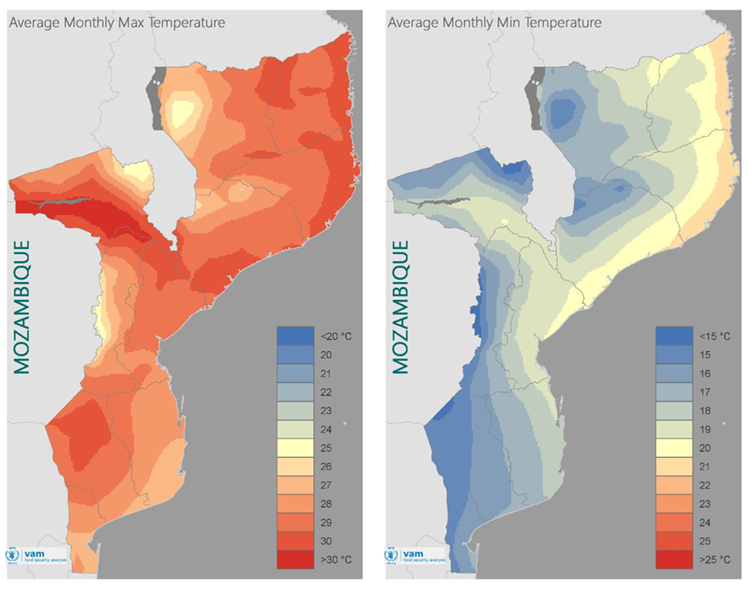
\includegraphics{Figure15.png}

\emph{Source: WFP, 2018. Mozambique Climate Analysis.}

\hypertarget{historical-trends}{%
\subsection{Historical Trends}\label{historical-trends}}

Average temperature trends show positive variations (increase in average temperature) in most parts of the country. Studies indicate that the average annual temperature increased by 0.6 °C between 1960 -- 2006, at an average rate of 0.13 °C per decade for most seasons of the year (INGC, 2009). The study also points to an increase in the frequency of hot days and nights (days with a maximum temperature\textgreater{} 30 °C and nights with a minimum temperature\textgreater{} 20 °C respectively). The average number of ``hot'' days per year in Mozambique increased by 6.8\% of days (\textasciitilde25 days) and the average number of ``hot'' nights per year increased by 8.4\% of nights (\textasciitilde31 nights) during the same period in analysis (1960 and 2006).

\emph{Maximum and minimum temperatures}

Trends in increasing maximum and minimum temperatures (warming) have not been uniform across the country. Increases in mean maximum temperature of greater magnitude were recorded in the North (0.76 -- 1.16 °C), followed by central Mozambique between 1960 and 2006. Changes in average minimum temperatures in certain regions of the country are even greater, indicating large increases between 1.12 - 1.62°C (in the central region of the country) during the same period under analysis (INGC, 2009). Tables 1.4 and 1.5 provide a summary of trends in average maximum and minimum temperatures for different regions of the country.

\emph{Table 1.4: Change in mean maximum temperature (Tmax, °C) for each region between 1960 and 2006}

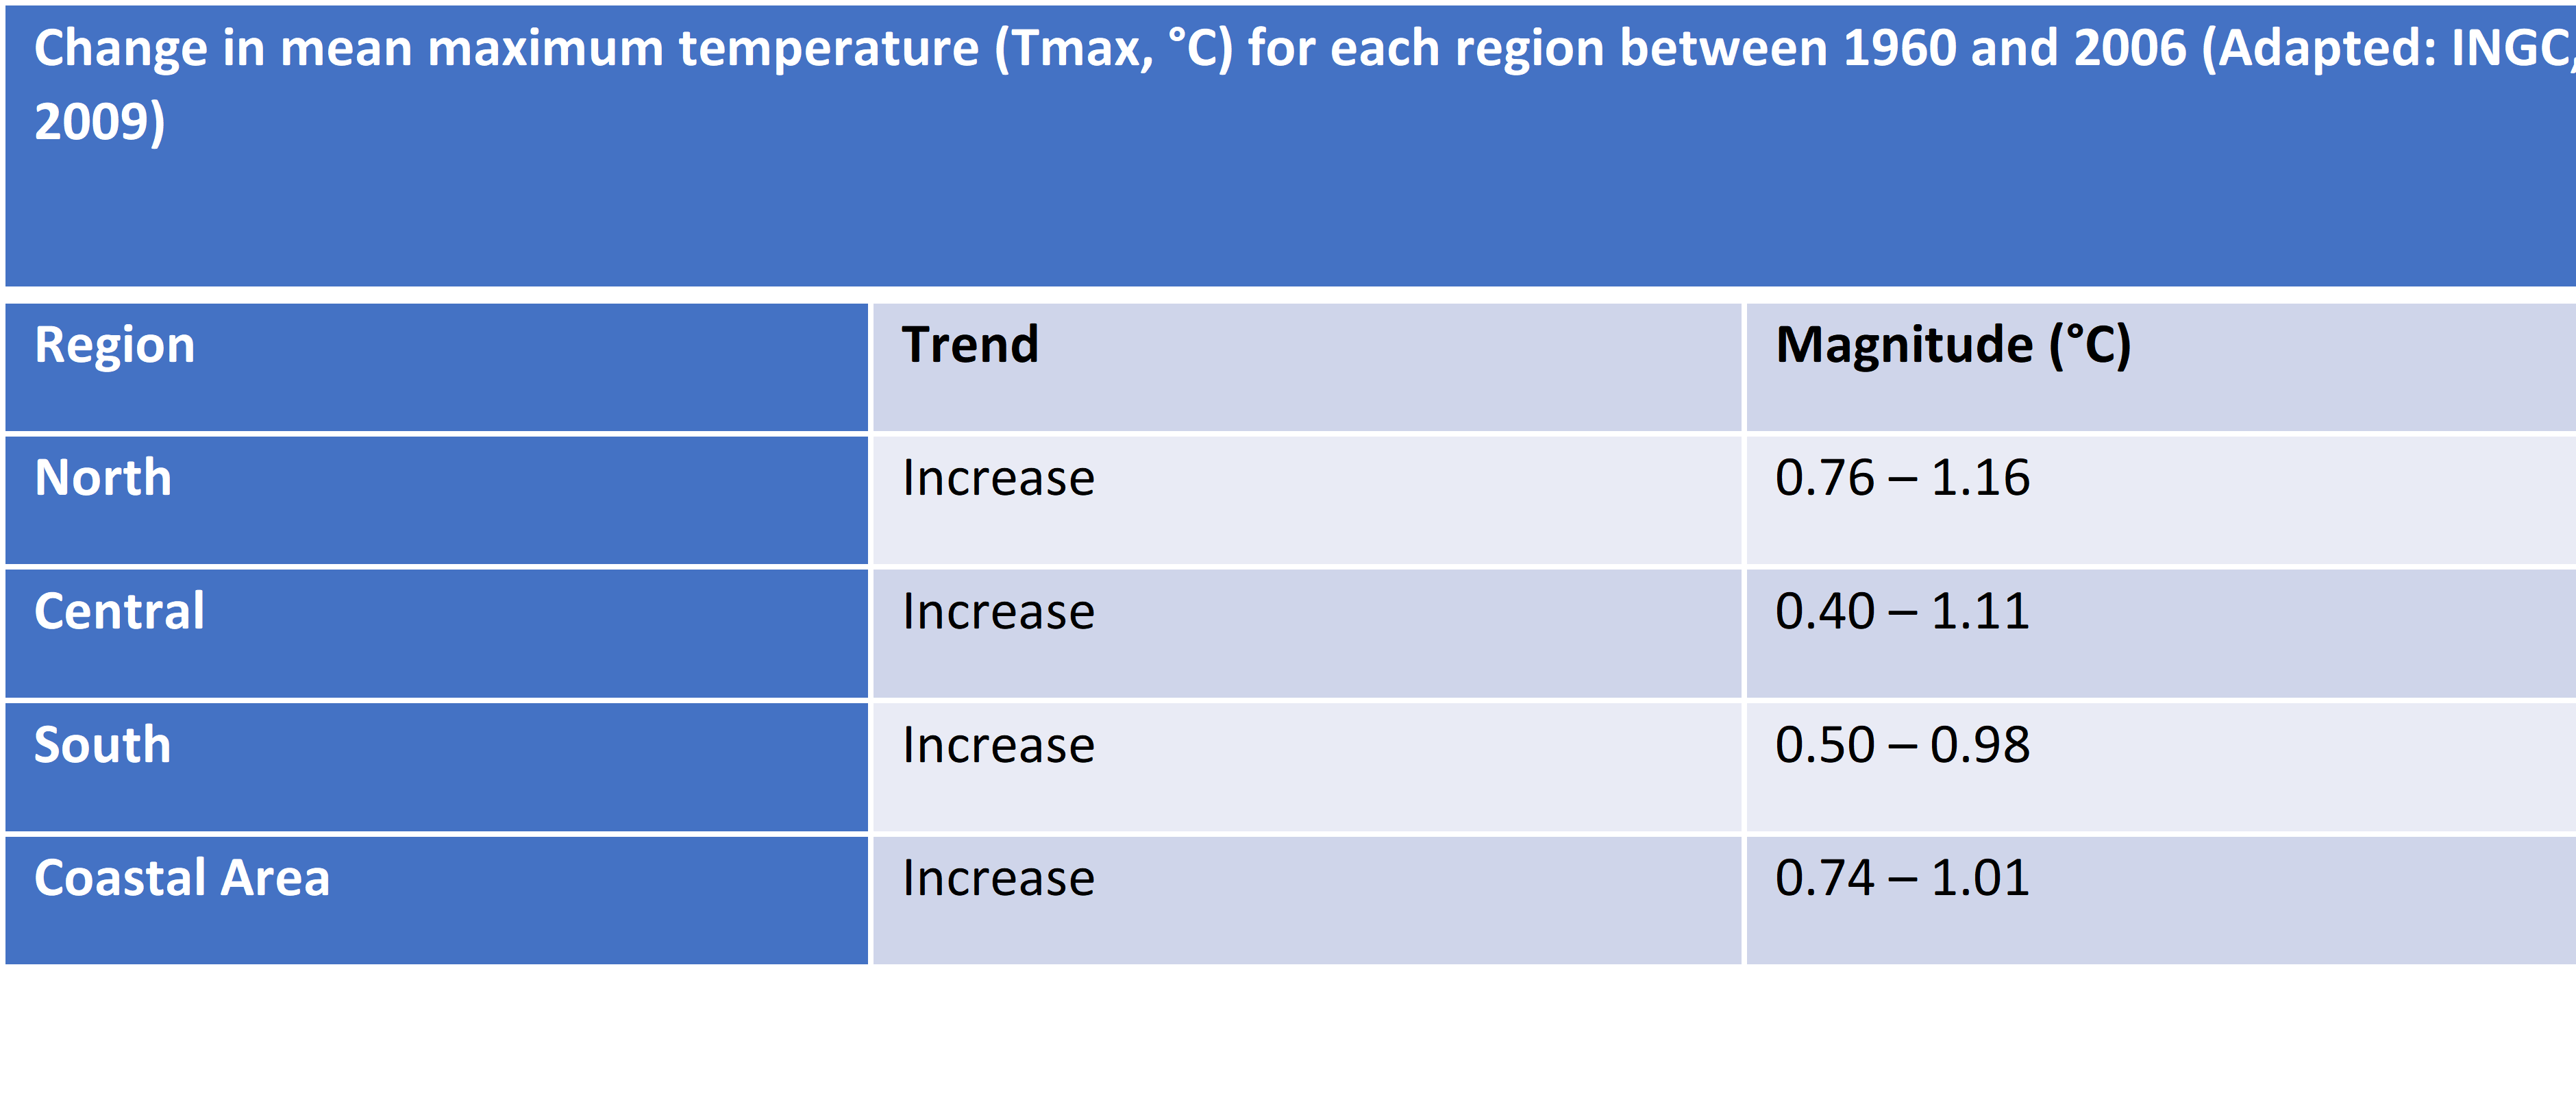
\includegraphics{Figure16.png}

\emph{Adapted: INGC, 2009}

\begin{center}\rule{0.5\linewidth}{0.5pt}\end{center}

\emph{Table 1.5: Change in mean minimum temperature (Tmin, °C) for each region between 1960 and 2006}

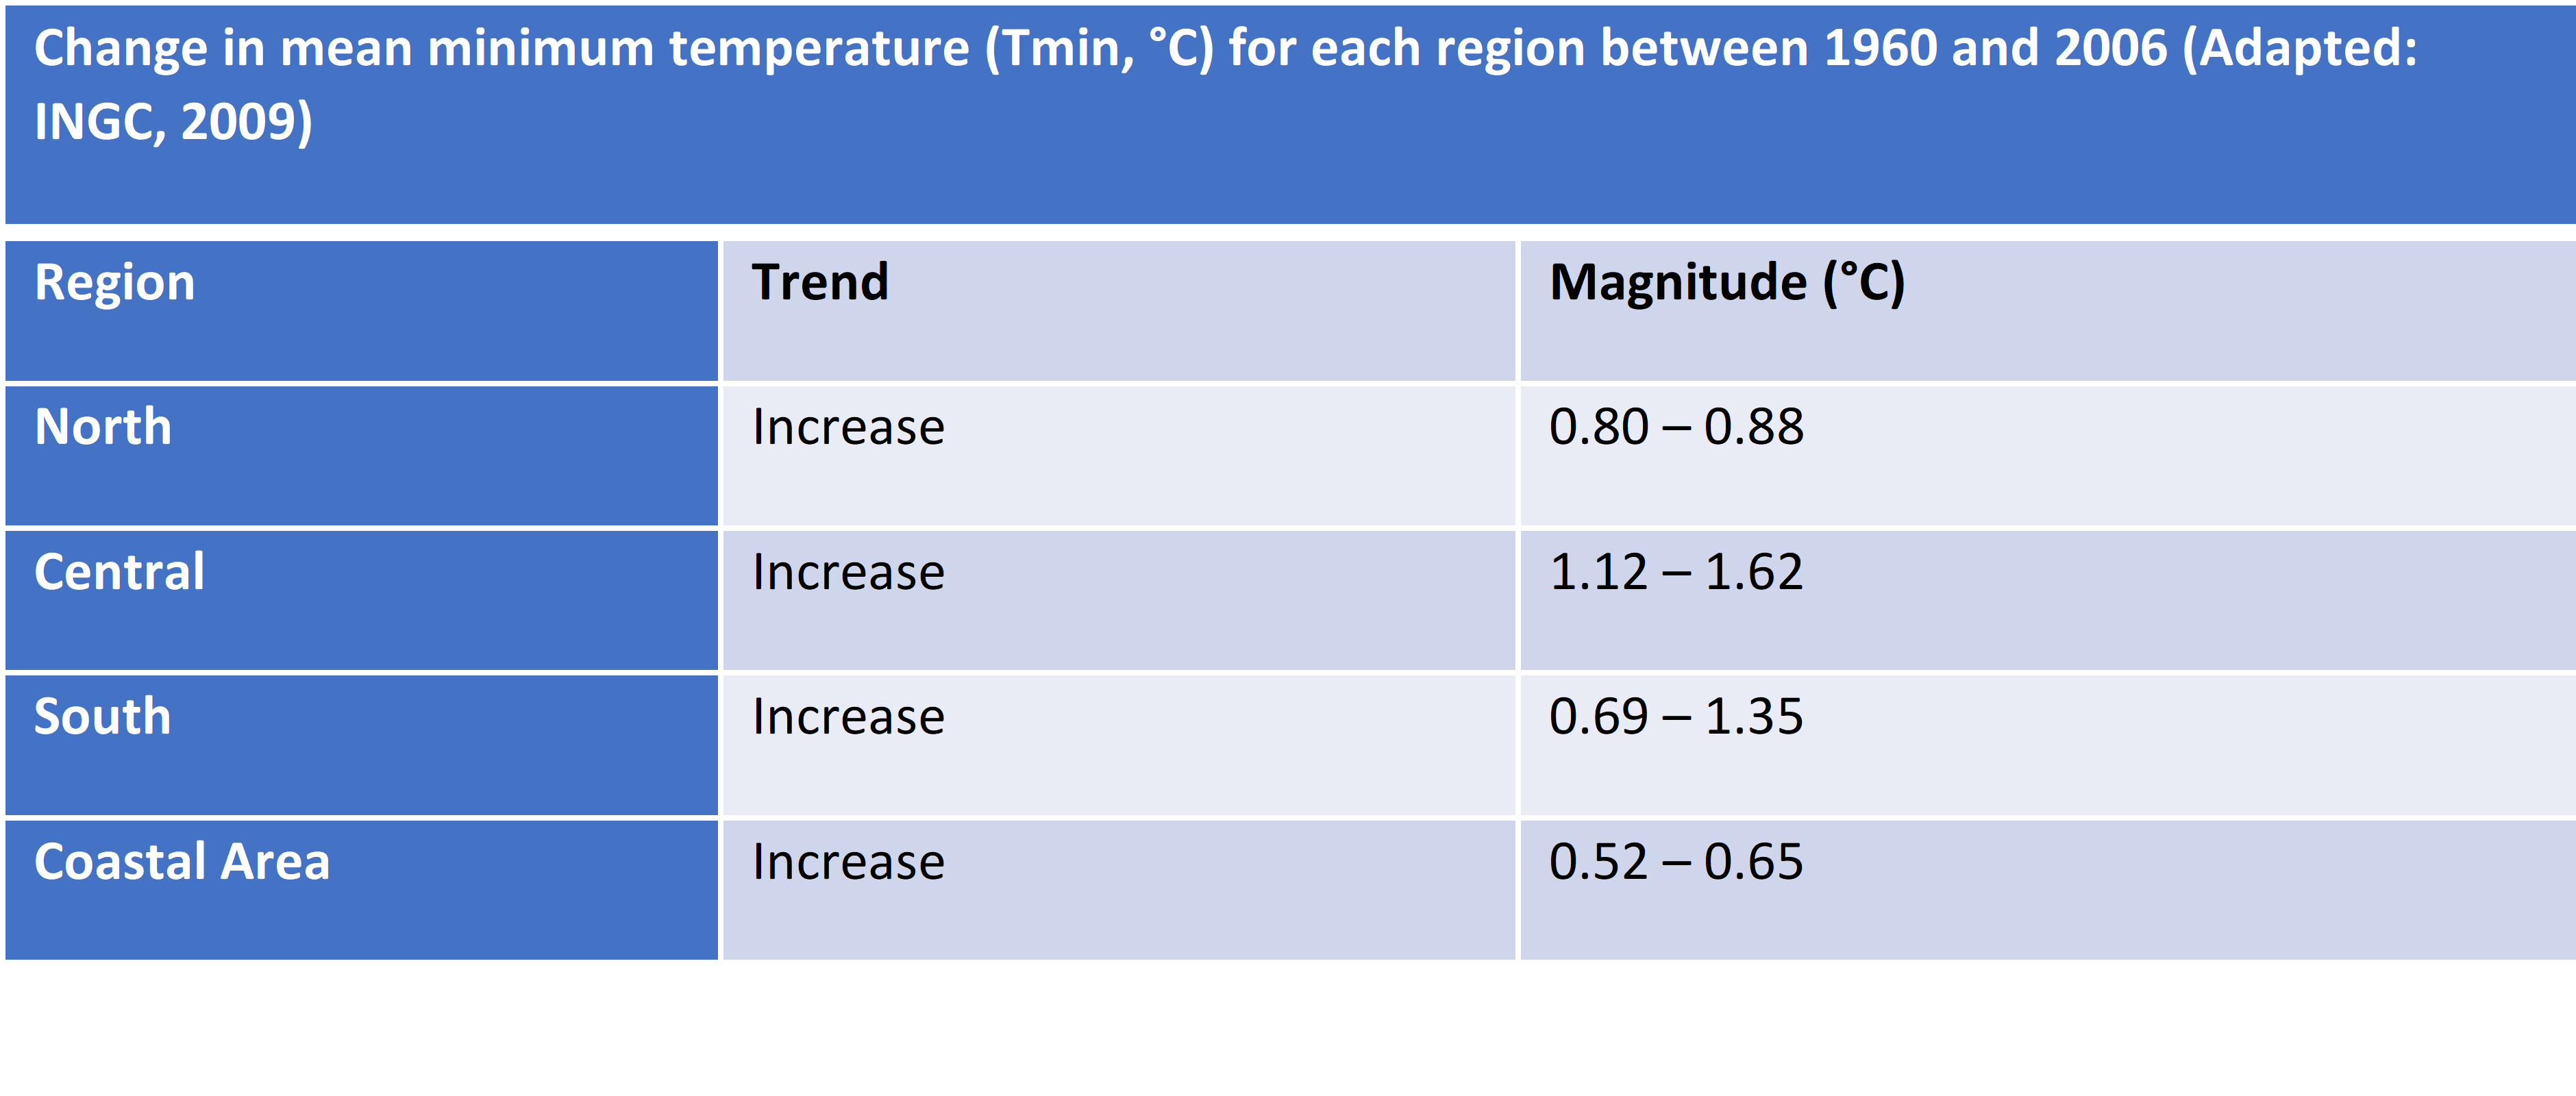
\includegraphics{Figure17.png}

\emph{Adapted: INGC, 2009}

\begin{center}\rule{0.5\linewidth}{0.5pt}\end{center}

\textbf{Precipitation Trends}

Precipitation trends in the country are not significantly observable, due to the great inter-annual variability of rainfall in different seasons. However, the analysis of historical data made in several studies points to a late start of the rainy season in Mozambique, as well as an increase in the persistence of dry days.

The INGC report (2009), analysing data between 1960 and 2006, indicates a delay in the start of the rainy season that can reach between 20 and 45 days in some places, as well as a more pronounced persistence of dry days in the Northeast of the country from March to May and September to November.

The study by Mcsweeney et al.~(2010) found that in the period between 1960 and 2006, the average annual rainfall in Mozambique decreased at an average rate of 3.1\% per decade, in the period under review. On the other hand, despite the decreases observed in total rainfall, the amount of rain falling during heavy rain events increased at an average rate of 2.6\% per decade, with these increases being more pronounced in the period from December to February (DJF ).

\hypertarget{climate-projections}{%
\section{Climate Projections}\label{climate-projections}}

\hypertarget{future-temperature-projections}{%
\subsection{Future Temperature Projections}\label{future-temperature-projections}}

The Intergovernmental Panel on Climate Change (IPCC) in its Fifth Assessment Report (AR5) presents unequivocal evidence of climate change around the world: the atmosphere and oceans are warming, the extent and volume of snow and ice is decreasing, sea levels are rising and weather patterns are changing. The most optimistic scenario predicts an increase in the Earth's temperature between 0.3 °C and 1.7 °C and, in the worst case scenario, the Earth's surface could warm between 2.6 °C and 4.8 °C over this century by 2100 (IPCC, 2014) . The Paris Agreement approved in December 2015 under the United Nations Framework Convention on Climate Change (UNFCCC) established a global framework to reduce carbon dioxide (CO2) emissions and noted that global warming should be limited to 1.5°C.
In Mozambique, some studies point to a significant increase in temperature, with the average annual temperature projected to increase between 1.0 to 2.8 °C by 2060 and between 1.4 to 4.6 °C by 2090 (INGC, 2009; Mcsweeney et al.~al., 2010) (figure 1.10). The projected rate of warming will be faster in inland Mozambique than in areas closer to the coast. All projections indicate substantial increases in the frequency of days and nights considered ``hot'' in the current climate. This increase will be between 17 and 35\% of days per year around 2060, and between 20 and 53\% of days per year in 2090. The same projections also indicate a reduction in the frequency of days and nights considered ``cold'' in the current climate.

\emph{Figure 1.10: Average annual temperature trends in Mozambique between 1960 and 2006 (black line) and the projected future for three emission scenarios (colored lines). The colored bars on the right side indicate the different scenarios used in the simulations (A2, A1B and B1) as well as the uncertainty ranges in the average climate projections around 2090 -- 2100}

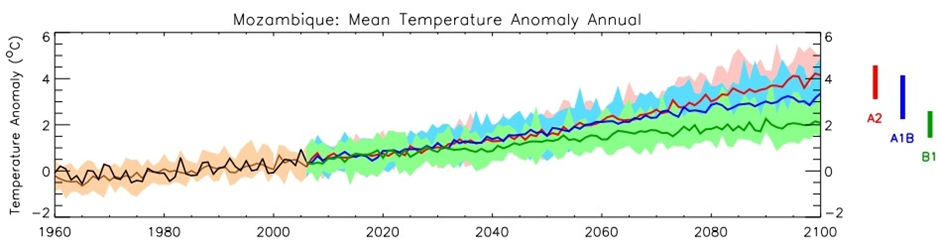
\includegraphics{Figure18.png}

\emph{Adapted from Mcsweeney et al., 2010.}

\hypertarget{future-precipitation-projections}{%
\subsection{Future Precipitation Projections}\label{future-precipitation-projections}}

Precipitation variations are not as clear as temperature variations. The range of precipitation projections resulting from different models is large and encompasses both negative and positive changes. There are indications of variations between -15 to +20 mm per month, or -15\% to +34\% (Mcsweeney et al., 2010). However, the models show more consistency in seasonal projections, indicating a reduction in rainfall in the dry season, that is, in the period from June to August (JJA) and from September to November (SON). This reduction is partially offset by increased rainfall in the rainy season, from December to February (DJF), with greater expression in northern Mozambique (Mcsweeney et al., 2010). In general, precipitation projections do not indicate substantial changes in annual precipitation, but rather changes in precipitation patterns (Figure 1.11).

\emph{Figure 1.11: Spatial patterns of monthly rainfall averages from September to November projected for the years 2030, 2060, and 2090}

\includegraphics{Figure19.png}

\emph{Adapted from Mcsweeney et al., 2010.}

\emph{(Source: Second National Communication Draft, p.~7-15. Translated from Portuguese)}

\begin{center}\rule{0.5\linewidth}{0.5pt}\end{center}

\hypertarget{our-analysis}{%
\section{(Our analysis)}\label{our-analysis}}

\hypertarget{nap-info}{%
\chapter{NAP Info}\label{nap-info}}

\hypertarget{vision-mission-and-goals}{%
\section{Vision, mission, and goals}\label{vision-mission-and-goals}}

\textbf{Vision:} ``A prosperous and climate change resilient Mozambique, with a green economy in all social and economic sectors''

\emph{(Source: National Climate Change Adaptation and Mitigation Strategy - 2012, p.27)}

\textbf{Mission:} ``reduce climate change vulnerability and improve the wellbeing of Mozambicans through the implementation of concrete measures for adaptation and climate risk reduction, promoting mitigation and low-carbon development, aiming at sustainable development, with the active participation of all stakeholders in the social, environmental and economic sectors''

\emph{(Source: National Climate Change Adaptation and Mitigation Strategy - 2012, p.27)}

\textbf{Goals:}

\begin{itemize}
\tightlist
\item
  Reduce climate risks through the strengthening of the early warning system and of the capacity to prepare and respond to climate risks;
\item
  Improve the capacity for integrated water resources management including building climate resilient hydraulic infrastructures;
\item
  Increase the effectiveness of land use and spatial planning (protection of floodplains, coastal and other areas vulnerable to floods);
\item
  Increase the resilience of agriculture, livestock and fisheries, guaranteeing the adequate levels of food security and nutrition;
\item
  Increase the adaptive capacity of the most vulnerable groups;
\item
  Reduce people's vulnerability to climate change related vector-borne diseases or other diseases;
\item
  Ensure biodiversity's protection;
\item
  Reduce soil degradation and promote mechanisms for the planting of trees for local use;
\item
  Develop resilient climate resilience mechanisms for infrastructures, urban areas and other human settlements and tourist and coastal zones;
\item
  Align the legal and institutional framework with the NCCAMS;
\item
  Strengthen research and systematic observation institutions for the collection of data related to vulnerability assessment and adaptation to climate change;
\item
  Develop and ameliorate the level of knowledge and capacity to act on climate change; and
\item
  Promote the transfer and adoption of clean and climate change resilient technologies.
\end{itemize}

\emph{(Source: Mozambique Intended Nationally Determined Contribution (INDC), p.6-7)}

\hypertarget{framework-for-the-nap}{%
\section{Framework for the NAP}\label{framework-for-the-nap}}

\hypertarget{the-national-adaptation-plan-process-in-mozambique}{%
\subsection{The National Adaptation Plan Process in Mozambique}\label{the-national-adaptation-plan-process-in-mozambique}}

Mozambique ratified the United Nations Framework Convention on Climate Change on August 24th, 1994 and became Party in 25th August 1995. In 2006, the country submitted its Initial National Communication to the UNFCCC which included, among others, information regarding greenhouse gases (GHG) inventory, vulnerability and adaptation (MICOA, 2003). In 2007, the National Adaptation Programme of Action (NAPA) was published including four initiatives to address the country's immediate and urgent adaptation needs on social and development sectors with a focus on agriculture, fisheries, energy, environment, water resources, coastal zones, disaster alert and early warning systems and erosion control (MICOA, 2007). With the objective to amplify efforts to tackle climate change impacts through adaptation and promote the development of a low-carbon economy, the National Climate Change Strategy 2013-2025 was published in 2012 recognizing climate risk reduction as a national priority (Ministry for the Coordination of Environmental Action, 2012). In October 2015, Mozambique published its INDC communicating the country's mitigation contribution and also including an adaptation component. According to the INDC, the implementation of the NCCAMS for the short term period (2013 -- 2019) was based on the implementation of Actions Plan aiming to increase local resilience, fight poverty, identify adaptation and low carbon development opportunities in the communities through the mainstreaming of adaptation in the planning and budgeting processes at the district level. The National Adaptation Plan (NAP) consist in the implementation of actions with the same objective as the Action Plans but for the medium term (2020 to 2025) at the provincial level, and for the long term (2026 to 2030) at the national level (Government of The Republic of Mozambique, 2015). Therefore, the present NAP document include the short term actions implemented at the local level and propose projects and programmes to be implemented for the period 2020 -- 2030 including provincial and national levels.

\hypertarget{essential-functions-of-the-nap-process}{%
\subsection{Essential functions of the NAP process}\label{essential-functions-of-the-nap-process}}

As part of the group of Least Developed Countries (LDCs), Mozambique has limited adaptive capacity due its low development levels, geographical location and socio-economic aspects. At the same time, is one of the most risk-prone countries in the world and the third African country most exposed to weather-related hazards and climate change impacts (Mozambique Crisis Response Plan 2020). The establishment of the NAP process in Mozambique aims to facilitate the integration of climate change adaptation into development planning and support the development and implementation of projects and programs aiming to reduce vulnerability to climate change impacts and build adaptive capacity and resilience. Following the (LDC Expert Group, 2012), the adaptation planning in Mozambique is intended to be a progressive and iterative process, based on national priorities reflecting plans, policies and strategies aiming to achieve sustainable development. It is guided by country-owned, country-driven, gender-sensitive and participatory approaches, based on the best available science and indigenous knowledge, with focus on the needs of vulnerable groups, communities and ecosystems.

\hypertarget{the-nap-as-the-umbrella-programme-for-adaptation}{%
\subsection{The NAP as the umbrella programme for adaptation}\label{the-nap-as-the-umbrella-programme-for-adaptation}}

\hypertarget{coherence-with-national-development-context-sdgs-sendai-and-other-relevant-frameworks}{%
\subsection{Coherence with national development context, SDGs, Sendai and other relevant frameworks}\label{coherence-with-national-development-context-sdgs-sendai-and-other-relevant-frameworks}}

\hypertarget{institutional-arrangements-and-coordination-mechanisms}{%
\section{Institutional Arrangements and Coordination Mechanisms}\label{institutional-arrangements-and-coordination-mechanisms}}

The Institutional arrangement emerges as an approach for better coordination and articulation among the various institutions/sectors. It aims at assigning responsibilities and hierarchical competences as well as defining standards/criteria for the flow and sharing of information. As a result, it is expected that climate change adaptation and mitigation actions will be implemented in an effective, transparent, coordinated way, and reinforcing the medium and long term action planning processes. The institutional arrangement is based on the National Strategy for Adaptation and Mitigation to Climate Change in Mozambique (MICOA, 2012) and consequently revised in the NDC Operational Plan (MITADER, 2018).

The institutional arrangement presented here has been adapted to reflect the current context of institutions facing climate change in sectoral activities and budget. To this end, the overall coordination lies with the Ministry of Land and Environment (MTA), through the National Directorate of Climate Change (DMC), which serves as the focal point for the convention.

The DMC is also responsible for coordinating the Inter-Institutional Group on Climate Change (GIIMC), which is composed of representatives from Ministries/Institutes whose mandates cover areas and/or sectors relevant to climate change, and representatives from non-governmental actors, the private sector, civil society, academia, and the media (figure 1.16).

\emph{Figure 1.16: Institutional Arrangements of ENAMMC and NDC Implementation Mechanisms. Source: adapted from MICOA, 2012 \& MITADER, 2018}

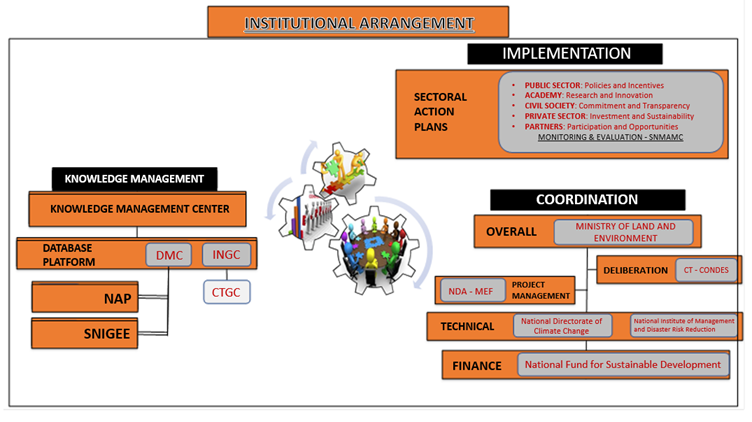
\includegraphics{Figure26.png}

Next, the key institutions are listed, containing the description of roles and responsibilities, related to the functions of proposing policies, strategies and decision-making, coordination, counseling and knowledge management, planning, communication, support mobilization, implementation of actions as described in table 1.6.

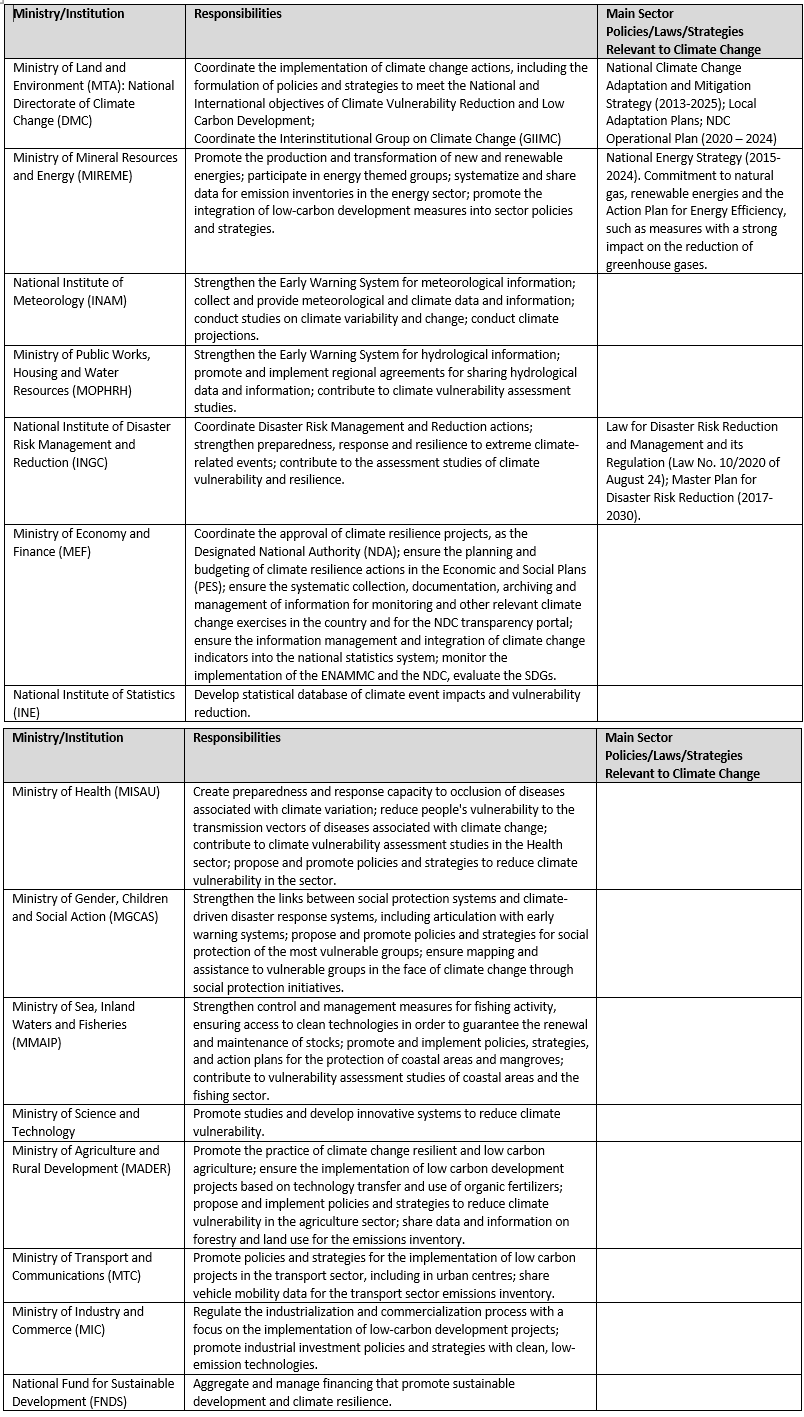
\includegraphics{Figure27.png}

These entities also play a key role in their contribution to:

\begin{itemize}
\tightlist
\item
  Harmonization of national actions and priorities considering the interests of different sectors and entities;
\item
  Appreciation and technical approval of documents prepared in the country, in the context of the implementation of the Convention and other instruments related to it;
\item
  Preparation of national and international climate reports; and,
\item
  Development of local initiatives for adaptation and mitigation to climate change, as well as for the promotion and continuous establishment of capacities, through studies and development of relevant courses.
\end{itemize}

\emph{(Source: Second National Communication Draft, p.~28-31. Translated from Portuguese)}

\hypertarget{current-climate-change-adaptation-projects-and-activities}{%
\section{Current climate change adaptation projects and activities}\label{current-climate-change-adaptation-projects-and-activities}}

\hypertarget{nap-approach}{%
\section{NAP Approach}\label{nap-approach}}

\hypertarget{guiding-principles}{%
\subsection{Guiding principles}\label{guiding-principles}}

\begin{itemize}
\tightlist
\item
  Proactive/Preventive nature -- demonstrate leadership and a pioneering spirit rather than a reactive attitude;
\item
  Social equity -- recognize and respect human rights and the fact that all citizens, regardless of their social status, should lead specific actions for mitigation and adaptation to CC, noting the cultural diversity that characterizes the Mozambican society;
\item
  Equality -- respecting the rights of men and women in all spheres of political, social, economic and cultural life, irrespective of colour, race, ethnic origin or place of birth, religion, level of education, socioeconomic status, occupation, political belief and party affiliation;
\item
  Gender parity -- respect the principle of equality between men and women, to ensure the representation of women in CC decision-making bodies and management;
\item
  Sustainability -- design CC interventions that are economically, financially, environmentally, socially and culturally sustainable;
\item
  Transparency and participation -- provide information exchange, accountability and adequate responses among different actors related to CC, to implement the Strategy through a broad, inclusive and participatory process.
\end{itemize}

\emph{(Source: National Climate Change Adaptation and Mitigation Strategy - 2012, p.27)}

\textbf{\emph{(Suggestion)}}

\begin{itemize}
\tightlist
\item
  Integration / mainstreaming
\item
  Inclusiveness / equity / vulnerability-focused - gender-sensitive / attention to vulnerable groups (women, children, youth, elderly, people with disabilities, indigenous people and traditional communities) / indigenous knowledge
\item
  Country-driven / country ownership / national context / national priorities
\item
  Transparency / good governance
\item
  Participatory / people-centered / social cohesion
\item
  Science and knowledge-based / ecosystem-based and community-based approaches
\item
  Principle of partnership
\item
  Innovation / technology
\item
  Flexibility
\end{itemize}

\hypertarget{a-systems-approach-to-adaptation}{%
\subsection{A systems approach to adaptation}\label{a-systems-approach-to-adaptation}}

The Government of Mozambique identifies climate shocks and seasonal variability, over exploitation of marine and timber resources, solid waste management, environmental sanitation and uncontrolled bush fires as major challenges.

\emph{Key economic sectors and systems}


\includegraphics{Figure20.png}

\emph{(Source: NAP Prototype, 25.09.2021, p.~21)}

\hypertarget{road-map}{%
\subsection{Road Map}\label{road-map}}

``Mozambique submitted the road map for the NAP to the UNFCCC and is receiving support from UNDP for the NAP process. With the assistance from UNDP, UN Environment National Adaptation Plan Global Support Programme (NAP-GSP) and additional financing from GIZ, the Mozambique Ministry of Land, Environment and Rural Development (MITADER) conducted training, connecting stakeholders from across the nation, with the aim to build a roadmap for a National Adaptation Plan. Mozambique has initiated the NAP process, an initiative which will contribute to a greater and deeper mainstreaming of climate change issues in the planning processes at all levels, in the medium and long-terms. The NAP road map was launched and the consultation process with national stakeholders and awareness of the NAP process started. The Government, working with UNDP and DANIDA submitted a proposal of \$3m to GCF to access the readiness funds''.

\emph{(Source: Mozambique Country Climate Risk Assessment Report, p.~28-29)}

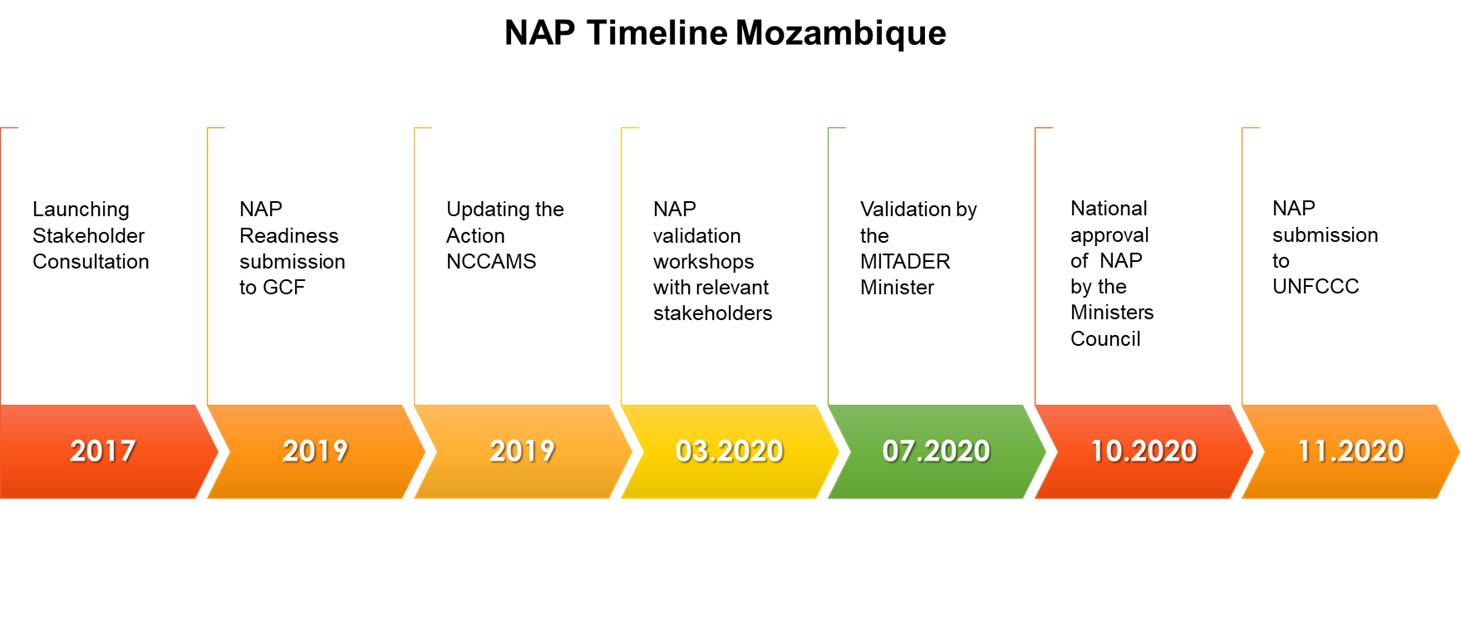
\includegraphics{Figure21.png}

\emph{(Source: NAP Prototype, 25.09.2021, p.~31)}

\hypertarget{vulnerabilities-and-impacts-assessment}{%
\chapter{Vulnerabilities and Impacts Assessment}\label{vulnerabilities-and-impacts-assessment}}

\hypertarget{vulnerabilities-impacts-and-risks}{%
\section{Vulnerabilities, impacts and risks}\label{vulnerabilities-impacts-and-risks}}

Mozambique is vulnerable to climate change due to its geographic location, low adaptive capacity as a result of poverty, limited investments in technology and weak infrastructure and social services. Climate change manifests through increased frequency and intensity of extreme events (droughts, floods, floods, event storms and tropical cyclones), rising sea levels, changes in temperature and precipitation patterns.

The consequences of the impacts of climate change include loss of human life, destruction of social and economic infrastructure, loss of domestic animals, loss of agricultural areas and crops, increased prices of agricultural products, deterioration of human health, environmental degradation with emphasis on erosion and saline intrusion.

This chapter presents the results of the vulnerability assessment and adaptation measures carried out in 2010, which covered the following sectors/areas: agriculture (maize cultivation in Chokwé); pastures and livestock, in the Limpopo basin; water resources, the Maputo basin was considered; fishing, shrimp in the Sofala bank; the coastal zone; mopane forests; and, health considered malaria and cholera. In the process of updating the SNA that started in 2020, other relevant sectors/areas were included, namely, biodiversity, infrastructure, energy and social protection, for which a review of the existing literature was carried out. Information on the impact of extreme events that occurred in the country in the sectors/areas covered was also included, using the Balance Sheet Reports of the Rainy Seasons produced by INGD.

Information on the vulnerability of the health sector was updated based on the preliminary results of the study ``Assessment of the Vulnerability and Adaptation to Climate Change of the Health Sector in Mozambique'' which includes the assessment of the impact of climate change on two climate-sensitive diseases in Mozambique: Malaria and Acute Diarrhea, carried out by MISAU.

In addition to the vulnerability assessment mentioned above, this chapter includes summary information on the vulnerability of 98 districts (Table 3.2) in which Local Adaptation Plans (PLAs) were formulated and approved within the scope of the implementation of ENAMMC. For the formulation of the PLAs in the districts, at least two communities in the district that participate in the assessment of the climate vulnerability and adaptability of the communities are involved -- Step 2 of the guide for the Formulation of Local Adaptation Plans. After the assessment with the communities, step 3 is followed, which is an assessment in the district. These two steps aim to determine the extent to which communities/districts are vulnerable to climate change, analysing trends, threats, opportunities and adaptive capacity of communities/districts to climate change and determining adaptation measures to improve their resilience to climate change.

The Guide for Formulating Local Adaptation Plans includes the Climate Vulnerability and Capabilities Analysis (CVCA) tools - developed by CARE and the Theory of Change (ToM). The PLAs are part of the short-term objectives defined by ENAMMC - increasing local resilience, fighting poverty and identifying opportunities for adaptation and low-carbon development at the community level, to be included in district planning.

\textbf{Climate Change Impacts}

\textbf{\emph{Disasters}}

Historical data on extreme events show that three climate-related hazards are most likely to occur in Mozambique, namely tropical cyclones, floods and droughts. These events are often associated with socio-economic damage, translated into loss of human life, human suffering, loss of assets, destruction of critical infrastructure (eg health facilities, schools, access roads, etc.) and other indirect losses.

An analysis of data from 1980 to 2019 shows that Mozambique was affected by 21 tropical cyclones, 20 flood events and 12 droughts (figure 3.1). This means that on average, the country is affected by a tropical cyclone or a flood event every two years and a drought event every three years. Tropical cyclones and flood events represent about 77\% of the total events that occurred in the period under review.

\emph{Figure 3.1: Total number of extreme events that occurred in Mozambique between 1980 -- 2019 }

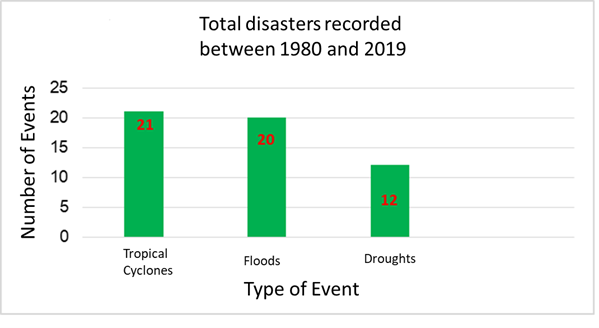
\includegraphics{Figure22.png}

\emph{Source: Produced based on DeSinventar data and INGC rainy season balance reports.}

\textbf{\emph{Historical trends of extreme events}}

One of the crucial questions today is whether there is any evidence of an increase in extreme disaster-causing events or not. Through an analysis of the trend of events registered in the last four decades (1980 -- 2019), it is noted that the number of events that devastated the country increased significantly since the 2000s (figure 3.2). From the decade (2000-2010) to the current, the number of cyclones competes with the number of flood events, despite the slowdown of drought events.

Taking into account that tropical cyclones are often associated with heavy rain events that can contribute a significant proportion of precipitation in a very short period which in turn cause flooding in various regions of the country, with serious implications for the health of communities, the worsening of these phenomena in recent decades should deserve special attention from health authorities and beyond.

\emph{Figure 3.2: Trend in the number of extreme events occurring between 1980 and 2019.}

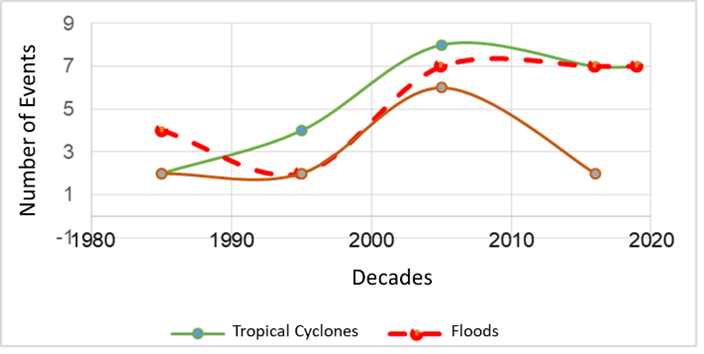
\includegraphics{Figure23.png}

The direct impact of these events is often expressed by the number of human lives lost, people affected through loss of personal property and livelihoods, destruction of the country's critical infrastructure such as roads, bridges, water supply system, schools, hospitals, as well as the outbreak of water-borne diseases (e.g.~malaria, cholera, diarrhoea, etc.). However, the lack of systematic and homogeneous recording of events and their impacts and, on the one hand, the persistence in considering only large-scale and high-impact disasters over a short period of time have hidden thousands of small and medium-scale disasters that occur every year in the country. Consequently, Mozambique does not know the real value of direct and/or indirect economic losses associated with these events.

Table 3.1 presents the impact of climate change on the human dimension. Regarding the economic impacts, these are presented in the respective sectors where the vulnerability analysis is carried out.

\emph{Table 3.1: Summary of impacts of extreme events on the human dimension}

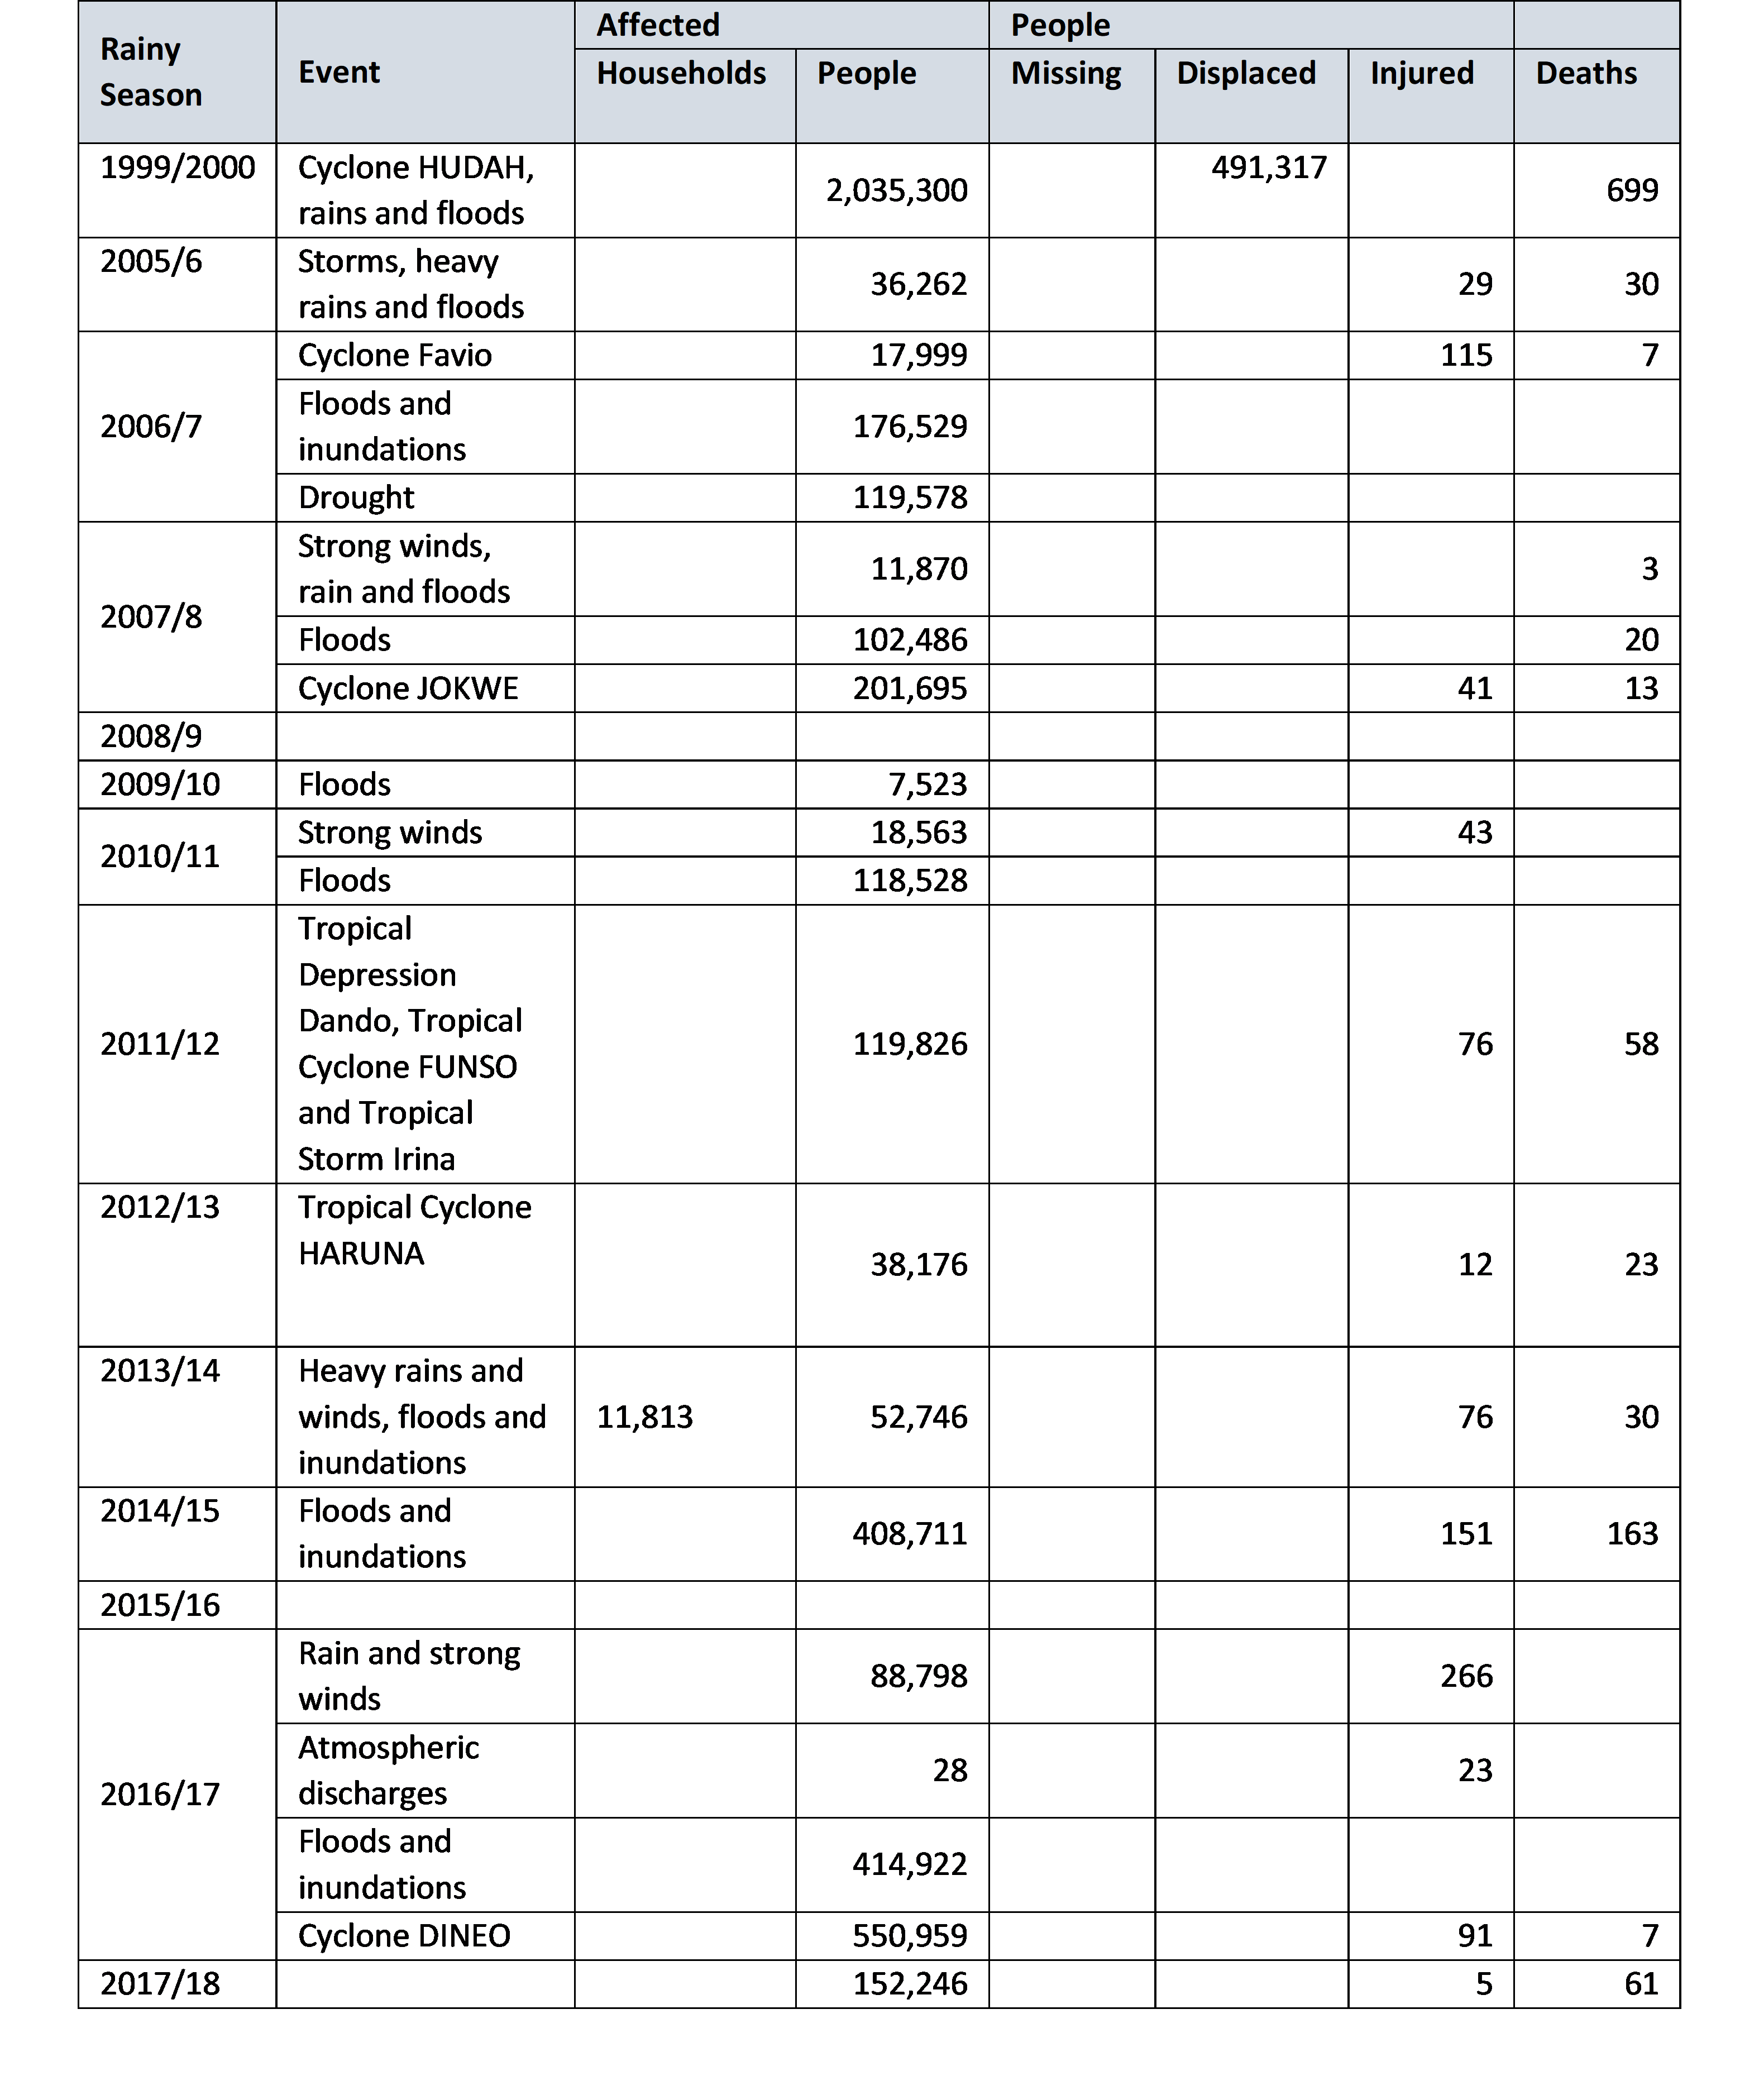
\includegraphics{Figure24.png}

\emph{Source: Rainy Season Balance Reports 2000, 2005/6 to 2017/18}

The extreme weather events that occurred in Mozambique in 2000 and in the rainy seasons from 2005/6 to 2017/18 affected an estimated 4,074,606 people, injured 885 people and caused 1,114 deaths. About 50\% of affected, injured and deaths resulted from the occurrence of Cyclone HUDAH, and it should be noted that tropical cyclones are events that cause greater impacts on the human dimension.

These impacts represent a setback in the process of poverty reduction, which is the priority of the Governments of developing countries, and increase their dependence on international aid. In this context, assessing the vulnerability of the most important social and economic sectors and identifying adaptation measures is of high priority.

\emph{Table 3.2: PLAs prepared in the period 2014 to 2018}


\includegraphics{Figure25.png}

The main threats indicated by communities and districts are grouped into droughts, floods and inundations, tropical cyclones/strong winds, sea level rise, epidemics, heat waves and/or cold spells, food insecurity, wildlife conflict and pests. (Include graph showing how each of the threats)

In addition to the PLAs, sector plans and other relevant instruments were also formulated, highlighting:

\begin{itemize}
\item
  The national action plan for the expansion of climate-resilient agriculture. This plan seeks to strengthen agricultural extension services to small farmers as well as knowledge management and sharing and strengthening in coordination with research and extension services;
\item
  Ministerial approval of national climate-resilient road standards and maintenance approaches; and the ministerial approval of mandatory climate risk screening for new road investments;
\item
  National Program for Productive Social Action (PNASP) through which households living in vulnerable districts are involved in public works activities in order to diversify their sources of income and, consequently, make them resilient.
\end{itemize}

\textbf{\emph{Climate Scenarios}}

The vulnerability analysis carried out at the SNC considered the climate projections developed by INGC ``Studies on the Impacts of Climate Change on Disaster Risk in Mozambique Synthesis Report -- Second Version'' in 2009.

The methodology of the INGC study was based on climatological modeling (temperature and rainfall) with the main purpose of understanding how Mozambique's climate may already be changing and how it can be expected to change in the future. This study details the observed changes in the country's seasonal climate during the period 1960 to 2005, in terms of temperatures and rainfall patterns (INGC, 2009).

Both historical trends and future projections were derived from daily temperatures (maximum and minimum) and rainfall values recorded since 1960, from 32 synoptic weather stations within Mozambique (INGC, 2009).

To project future scenarios in terms of the country's climate (temperature and rainfall), focusing on the mid-century (2046-2065) and late-century (2080-2100) periods, seven general circulation models were used: ECHAM, GFDL , IPSL, CCCMA, CNRM, CSIRO and GISS.

INGC's projections (2009) anticipate that climate change in Mozambique is mainly manifested in the following:

\emph{Temperature patterns}

\begin{itemize}
\item
  Atmosphere -- with an average increase between 1.5ºC and 3.0ºC in the period between 2046 and 2065 and recording of more hot days and fewer cold days, with an increase in the maximum and minimum temperature;
\item
  Oceans -- with rising mean sea levels and changes in the distribution and availability of fish stocks and effects on marine ecosystems (such as corals);
\end{itemize}

\emph{Precipitation patterns}

\begin{itemize}
\item
  With irregular rainfall behavior in terms of start and end times, rainfall (heavy precipitation phenomena in a short space of time) and duration of the rainy season (drought), disfiguring the notions of ``official'' and ``real'' start of the agricultural season, which may result in some regions in a decrease in current potential yields of around 25\%;
\item
  With a growing reduction in potential agricultural income levels of up to 20\% in the main crops that constitute the basis of food security and an essential condition for improving the per capita income of Mozambican families;
\end{itemize}

\emph{Increased frequency and intensity of extreme events (droughts, floods and tropical cyclones)}

\begin{itemize}
\item
  Persistence of the situation of extraordinary floods in identifiable places in the country which can be referred to as ``risk zones'';
\item
  Cyclones and other strong winds;
\item
  Prolonged droughts;
\end{itemize}

\emph{Sea level rise:}
15 cm, 30 cm and 45 cm as a consequence of thermal expansion and 15 cm, 110 cm and 415 cm as a consequence of the reduction of continental ice caps in the years 2030, 2060 and 2100, respectively;

\begin{itemize}
\item
  Areas with potential increased risk identified due to the emergence of other adverse natural phenomena such as loss by submersion and erosion of coastal areas, intrusion of saline water, desertification;
\item
  Reduction of areas available for agricultural practice in green or low-lying areas;
\item
  Many of the country's main coastal urban centers, including Maputo, Beira and Quelimane, are already in a critical situation in terms of vulnerability (human lives, properties, social infrastructure, etc.) to the effects of climate change.
\end{itemize}

\emph{(Source: Second National Communication Draft, p.~131-137. Translated from Portuguese)}

\begin{center}\rule{0.5\linewidth}{0.5pt}\end{center}

\textbf{Climate change impacts: highlights of recent impacts:}

\begin{itemize}
\item
  Mozambique is particularly vulnerable to Climate Change (CC) due to its location downstream of shared watersheds (Floods, e.g.~2000 and 2013 Limpopo Basin; 2007 Zambeze, 2013 and 2019 Licungo Basin, etc.)
\item
  Increase in the frequency and intensity of extreme climatic events, such as droughts, floods and tropical cyclones (recent cyclones with high impact: Idai and Keneth 2019, Eline in 2000, etc.)
\item
  The long shoreline and the existence of extensive low-lands below sea level (sea level rise, storm surge, salt intrusion);.
\item
  The country's vulnerability is also increased by its low adaptive capacity, poverty, limited investment in modern technology, and weaknesses in its infrastructure and social services, especially those related to health and sanitation (e.g.~the malaria and cholera in 2019 after the cyclone Idai and Keneth in central and northern Mozambique).
\item
  These events result in the loss of human lives, crops, livestock and wildlife; the destruction of social and economic infrastructure; increased dependency on international support; food price increases; harm to human health and the environment; and the destruction of ecosystems.
\item
  CC represents a major barrier to the Government and its partners' efforts to fight poverty and achieve the MDGs.
  (Government of Mozambique, 2012)
\end{itemize}

\emph{(Source: NAP Prototype, 25.09.2021, p.~22)}

\hypertarget{main-hazards}{%
\section{Main Hazards}\label{main-hazards}}

The main hazards in Mozambique are tropical cyclones, drought and floods . Cyclones pose significant risks for the population in coastal regions, may occur during the hot, humid season and may last few days. Many people are affected by drought every year, specially the poor and rural population dependent on rain-fed agriculture (Ministry of Foreign Affairs of the Netherlands, 2018). As a slow-onset hazard, droughts often las more than an year and may cause longer-term impacts and economic disruption compared to rapid onset hazards as floods (Pereira et al.~2011). Floods pose risks to lowland, highland and urban areas, and occur commonly followed by a tropical cyclone. Landslides affect a smaller number of people (Ministry of Foreign Affairs of the Netherlands, 2018).

\hypertarget{cyclones}{%
\subsection{Cyclones}\label{cyclones}}

\hypertarget{drought}{%
\subsection{Drought}\label{drought}}

Droughts are sustained periods of below water availability (The World Bank, 2019). It may have natural or anthropogenic causes, the first may be associated to changes in the precipitation regime and El Niño conditions, and the second due to excessive use of soils for agriculture, the industrial forestry sector, bush fires, over grazing, land degradation, among others. The cause is also linked to the community poverty levels, what can result in the overuse of land resources. Droughts and desertification have high economic and social costs, including loss of livelihood, employment, migration, loss of crops, drying of water resources, negative impacts on coastal zones and the fishery sector, higher costs of food and agricultural products, need of external aid, increase in food imports, disease outbreaks, loss of biodiversity, human and animal lives (MICOA, 2007).

As the most frequent disaster (occurring every three to four years), droughts pose a major challenge for Mozambique's development, affecting mainly the poor population living in rural area which rely on rain-fed agriculture (Ministry of Foreign Affairs of the Netherlands, 2018). Droughts are more frequent in the southern and central regions, and may be associated to the phenomenon of El Niño (warming of the waters of Equatorial Pacific) and La Niña (cooling of the waters of Equatorial Pacific). Droughts affect relevant development sectors resulting in negative impacts as water scarcity, agricultural losses and food insecurity.

\hypertarget{floods}{%
\subsection{Floods}\label{floods}}

\hypertarget{climate-change-adaptation-assessment}{%
\section{Climate Change Adaptation Assessment}\label{climate-change-adaptation-assessment}}

\hypertarget{priority-sectors}{%
\chapter{Priority Sectors}\label{priority-sectors}}

\hypertarget{agriculture-and-livestock}{%
\section{Agriculture and Livestock}\label{agriculture-and-livestock}}

\begin{itemize}
\tightlist
\item
  \textbf{Objective: Increase the resilience of agriculture and livestock}
\end{itemize}

\hypertarget{context}{%
\subsection{Context}\label{context}}

Agriculture in Mozambique is the basis for development, constituting the most important source of income and subsistence for more than 80\% of the population and with an average share of GDP above 20\% of the total (INE: National Accounts, 2008 -- 2018 ). The agriculture sector also plays an essential role for women's livelihoods, as 90\% of the economically active female population earns a living from agriculture. Furthermore, women constitute 61\% of the agricultural workforce. The country's agricultural potential is estimated at 62\% of the total area, but only 7\% of the area is currently cultivated (CIAT; World Bank. 2017). Of the 3 million hectares of land with potential for irrigated agriculture, only 118,000 hectares were equipped for irrigation in 2015 and only 62,000 ha (52\%) were being used for irrigated agriculture (CIAT; World Bank. 2017). The country's National Development strategy (2015-2035), the Green Economy Action Plan (2013-2030), the National Climate Change Adaptation and Mitigation Strategy (2013-2025), identify the agriculture sector as essential for poverty reduction and to stimulate economic growth, as well as the one with the greatest potential for adaptation and emission reduction through the promotion of resilient production techniques and systems.

The staple food production is dominated by cereals such as maize, sorghum, millet and rice. Rice production has shown great expression in recent years with the expansion of national production on a commercial scale. Regarding cash crops, cotton, sugar cane and tobacco are the most expressive crops both in terms of area covered and production volume. Rice production is carried out in irrigated areas and flood plains. Rice constitutes the third most important crop in the group of cereals, having increased the cultivated area from 200,000 hectares in 2006 to 300,000 hectares in 2012, although the national potential is about 900,000 hectares.

Agriculture in Mozambique is mainly dominated by the family sector whose production is subsistence-oriented, rainfed, and highly vulnerable to climate variability. In terms of farm size, approximately 72\% of the country's farmers work on plots of land that do not exceed 2ha, using limited amounts of inputs and practicing extensive slash and burn (CIAT; World Bank. 2017). Livestock production and savannah burning represent two main sources of greenhouse gas (GHG) emissions in the agriculture sector.

Livestock production is a relevant activity in the agricultural sector. Animal husbandry is a component of diversification of peasants' livelihoods, constitutes a source of income and an economic reserve, contributes to the balance of production systems, to increase agricultural production, with animal traction and manure, and for the food security of families, playing a social role in rural communities. Livestock production is mainly carried out by the family sector for subsistence (mainly small animals such as goats, rabbits, chickens, ducks), but large-scale production has been increasing in recent years, mainly cattle (cattle, pigs, goats and sheep) and broilers and egg production.

Although agriculture is the economic base of the majority of the country's population, it is constrained by low soil productivity; biotic and abiotic factors such as high pest, disease and weed pressure, and irregularity and scarcity of rainfall, respectively; low use of inputs (fertilizers, pesticides and improved seed); and the low level of use of appropriate technologies. Other factors that also contribute to low productivity include poor agronomic practices and insufficient extension services due to low geographical coverage.
Vulnerability to Climate Change and Disasters

\emph{(Source: Second National Communication Draft, p.~17-18. Translated from Portuguese)}

\hypertarget{vulnerability-to-climate-change-and-disasters}{%
\subsection{Vulnerability to Climate Change and Disasters}\label{vulnerability-to-climate-change-and-disasters}}

Agriculture is considered to be the basis for Mozambique's development. This sector is made up of small, medium and large producers. The most predominant class is smallholders who use approximately 97\% of the approximately five million arable land currently used for agriculture (Mozambique Government - PAPA, 2008).

In 2010, agriculture contributed 23\% to the Gross Domestic Product (INE). Furthermore, 80\% of the country's active population is employed in the agrarian sector. Thus, this sector is fundamental for poverty reduction and income generation for rural families, since most of this population depends on agriculture for food, employment and income.

A critical factor in agricultural production is access to and distribution of water throughout the vegetative cycle of crops. Production and productivity levels are affected by changes in climatic parameters, in particular variations in rainfall, given that around 98\% of farmers practice rainfed agriculture (CAP, 1999-2000).

According to the rainy season balance sheets, the agriculture sector is vulnerable to drought and drought events, floods and inundations, strong winds, tropical cyclones including pests (see Table 3.3). These events result in crop areas affected and/or lost; death and/or disappearance of domestic animals, especially cattle, goats, pigs, sheep and poultry; destruction of agricultural and animal management infrastructures; loss of pasture areas, affecting farmers and their families.

\emph{Table 3.3: Impact of climate change on agriculture}

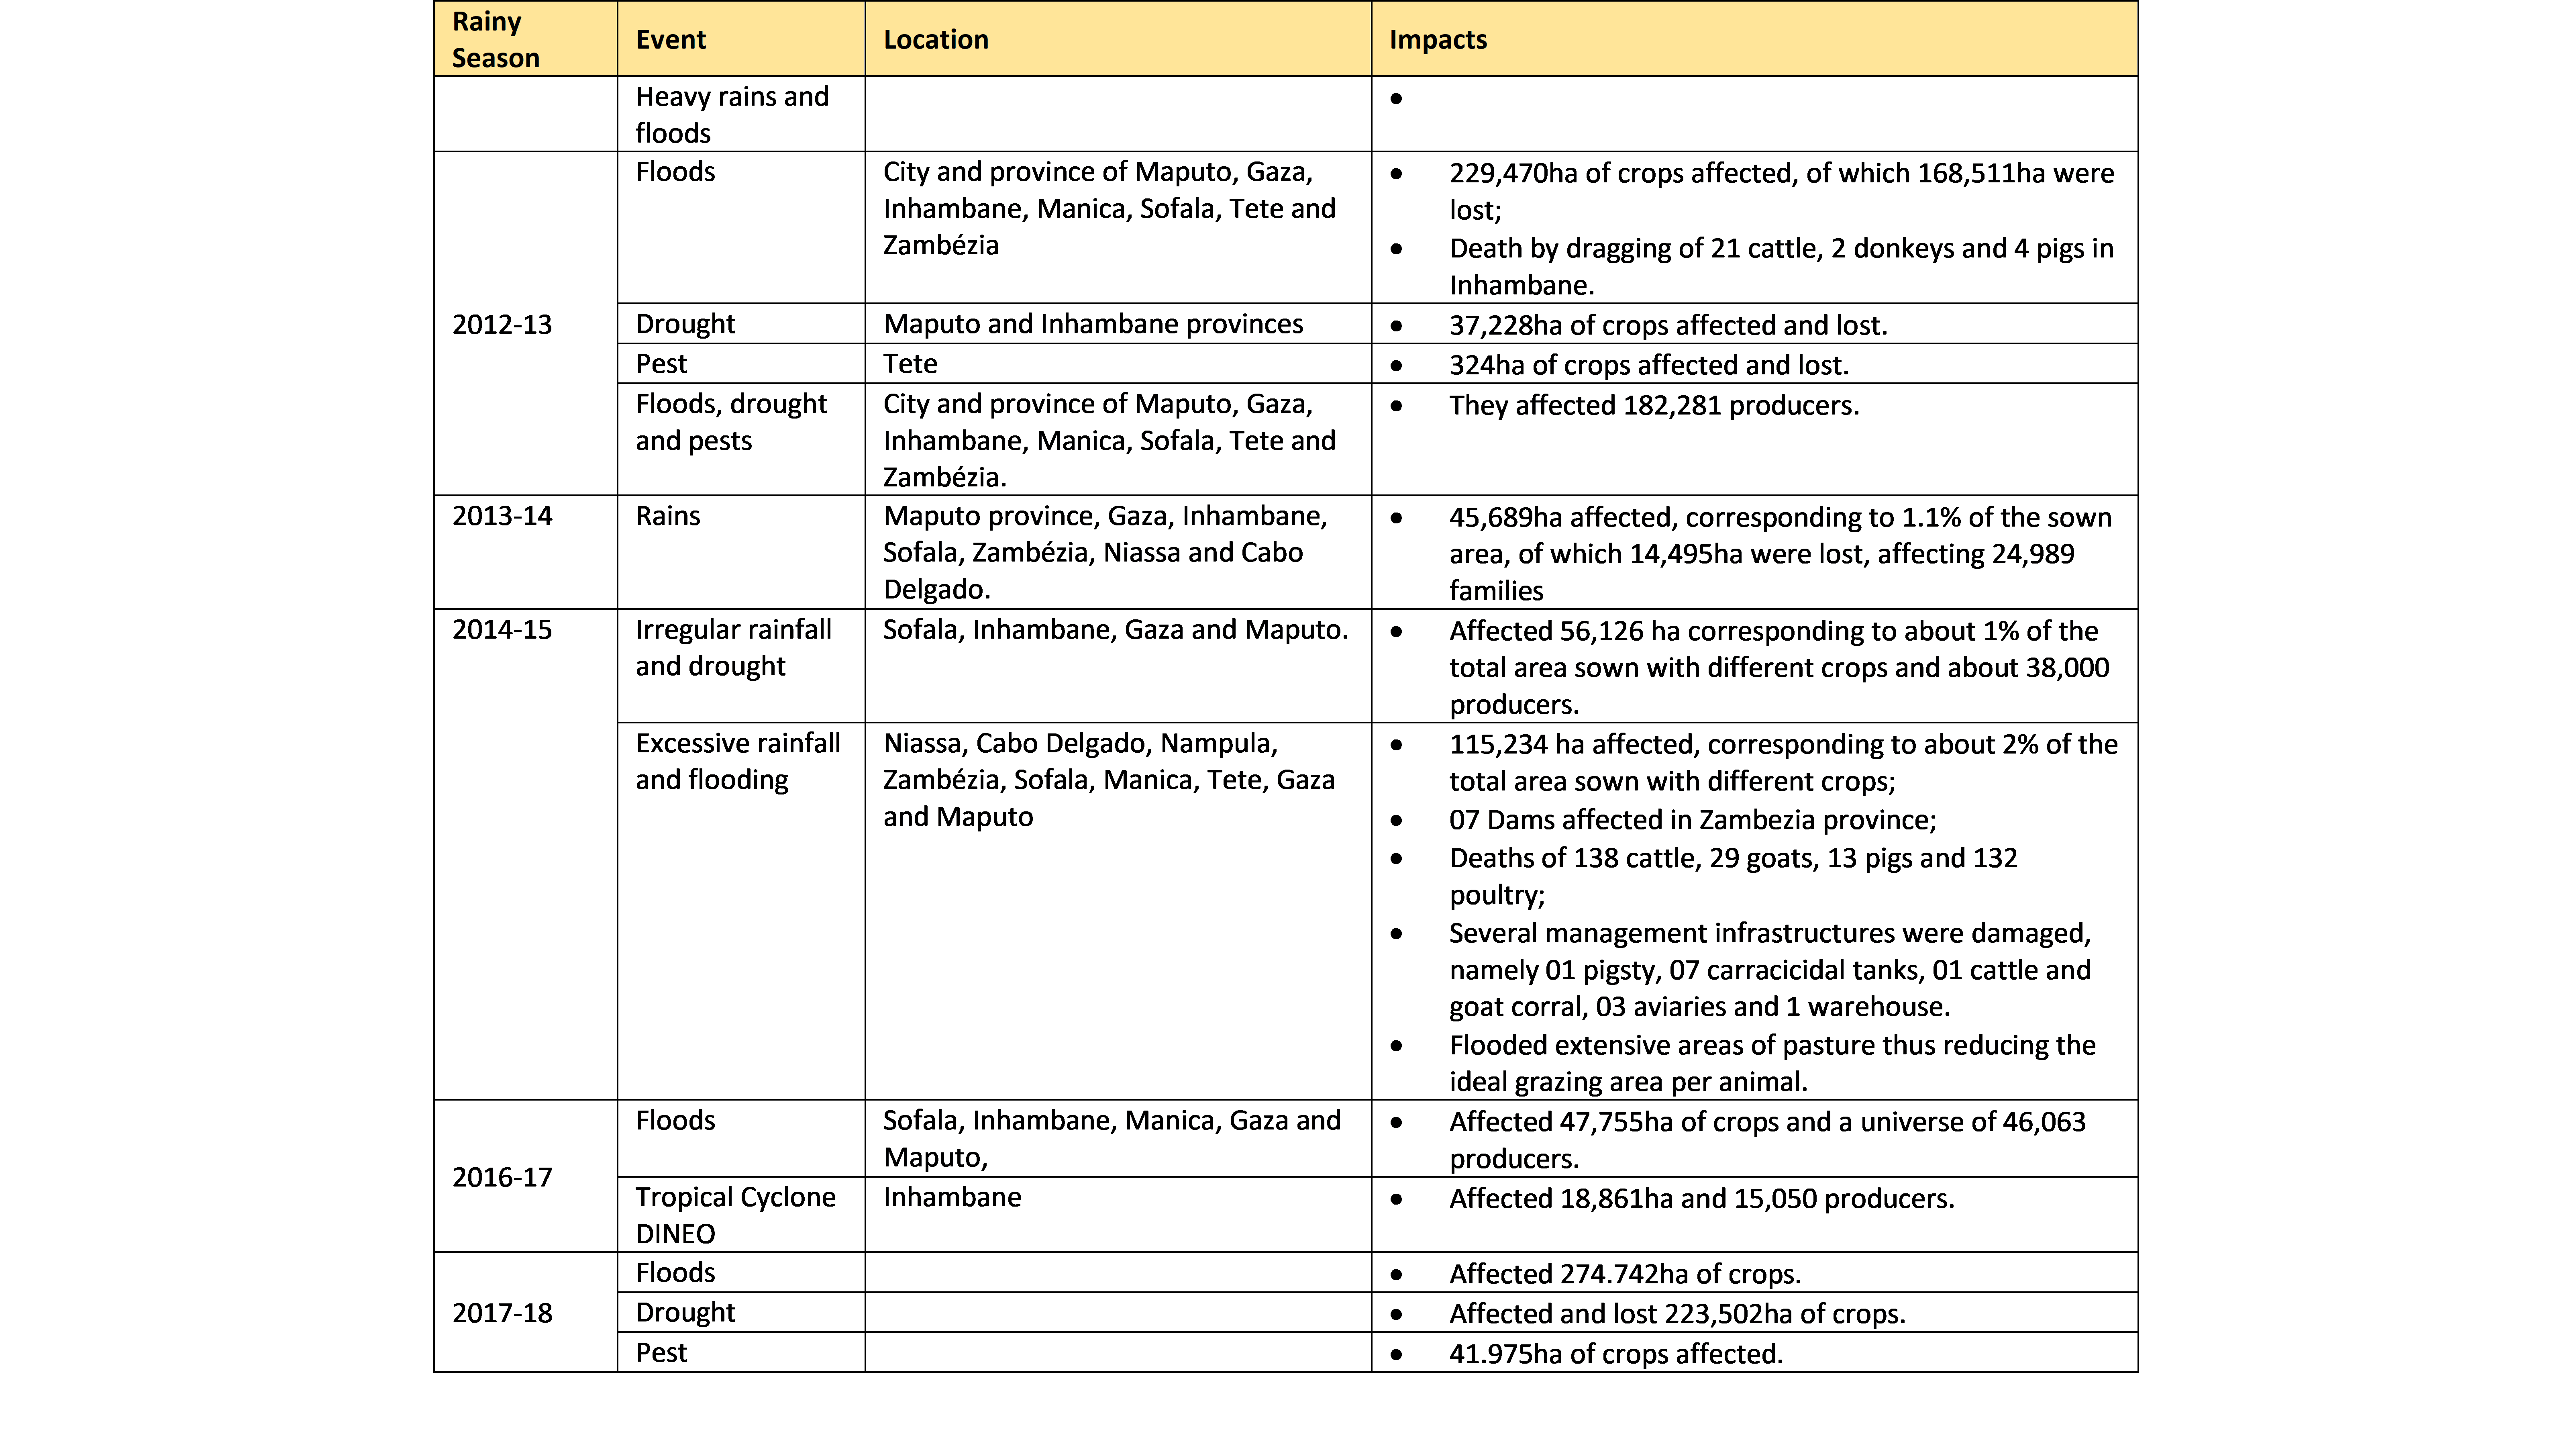
\includegraphics{Figure28.png}

\emph{Source: Balances of the rainy seasons for the period 2011-12 to 2017-18}

Weather events in the country between the rainy seasons from 2011-12 to 2017-18 affected around 1,384,677 ha of crops, of which around 733,270 ha were lost. The events that affected the largest area of crops were the tropical depression Dando and the tropical cyclone Funso, which occurred in the 2011-12 rainy season, while the greatest loss of crops occurred following the floods of 2012-2013.

The events that cause most loss and destruction in the agricultural sector are those related to excessive rainfall and floods and tropical cyclones. However, when a drought occurs, usually the area affected equals the area lost.

It is also important to stress that in addition to the biophysical vulnerability associated with the occurrence of extreme weather events, the levels of technology adopted by most producers do not correspond to the requirements of the selected varieties, due to the weak financial capacity to purchase agricultural inputs, which also contributes to low production and productivity.

Livestock plays a vital role for the rural population, it is one of the components of agriculture. The contribution of livestock to the national economy is incipient. In 2008, livestock represented 10\% of total agricultural production and contributed only 1.7\% to the Gross Domestic Product (OIE Report, 2008). However, animal production is affected by climate change in food quantity and quality, disease distribution, management practices and production systems (Herrero et al.~2009).

The main constraints to the development of livestock production are as follows:

\begin{enumerate}
\def\labelenumi{(\roman{enumi})}
\item
  Low productivity of existing herds due to the genetic quality of breeding stock and inadequate management practices;
\item
  Weak veterinary assistance network for the family sector;
\item
  Lack of infrastructure for watering and managing livestock.
\end{enumerate}

PEDSA identifies drought as one of the environmental factors causing a notable loss of productivity and the use of technologies to improve water availability and management as a key element to improve livestock production. For example, in 2015, 6,767 cattle and 112 goats died nationwide due to drought.

In semi-arid regions, livestock production is a way for farmers to adapt to climate change, as animals are relatively less affected. However, several aspects of livestock production are affected by climate change, including feed quantity and quality, disease distribution, management practices and production systems (Herrero et al.~2009). Therefore, to achieve the above Government objectives, investment is needed to address any constraints to livestock productivity, including climate change.

The vulnerability and adaptation of pastures and livestock are matters of great concern in developing countries such as Mozambique, due to the great importance of livestock as a livelihood component and source of income for local communities. The objectives of this sub-chapter are:

\begin{enumerate}
\def\labelenumi{(\arabic{enumi})}
\item
  Assess the expected impacts and vulnerability of pasture and livestock to climate change;
\item
  Identify adaptation programmes and measures;
\item
  Identify gaps, needs and priorities for climate change education, training and public awareness.
\end{enumerate}

It should be noted that the impacts of extreme climate events on livestock are already a reality in the country, as illustrated in Table 3.4. The observed impacts range from the loss of animals through death to the destruction of livestock management infrastructures, including the loss of pasture areas.

\emph{Table 3.4: Impacts of extreme events on livestock}

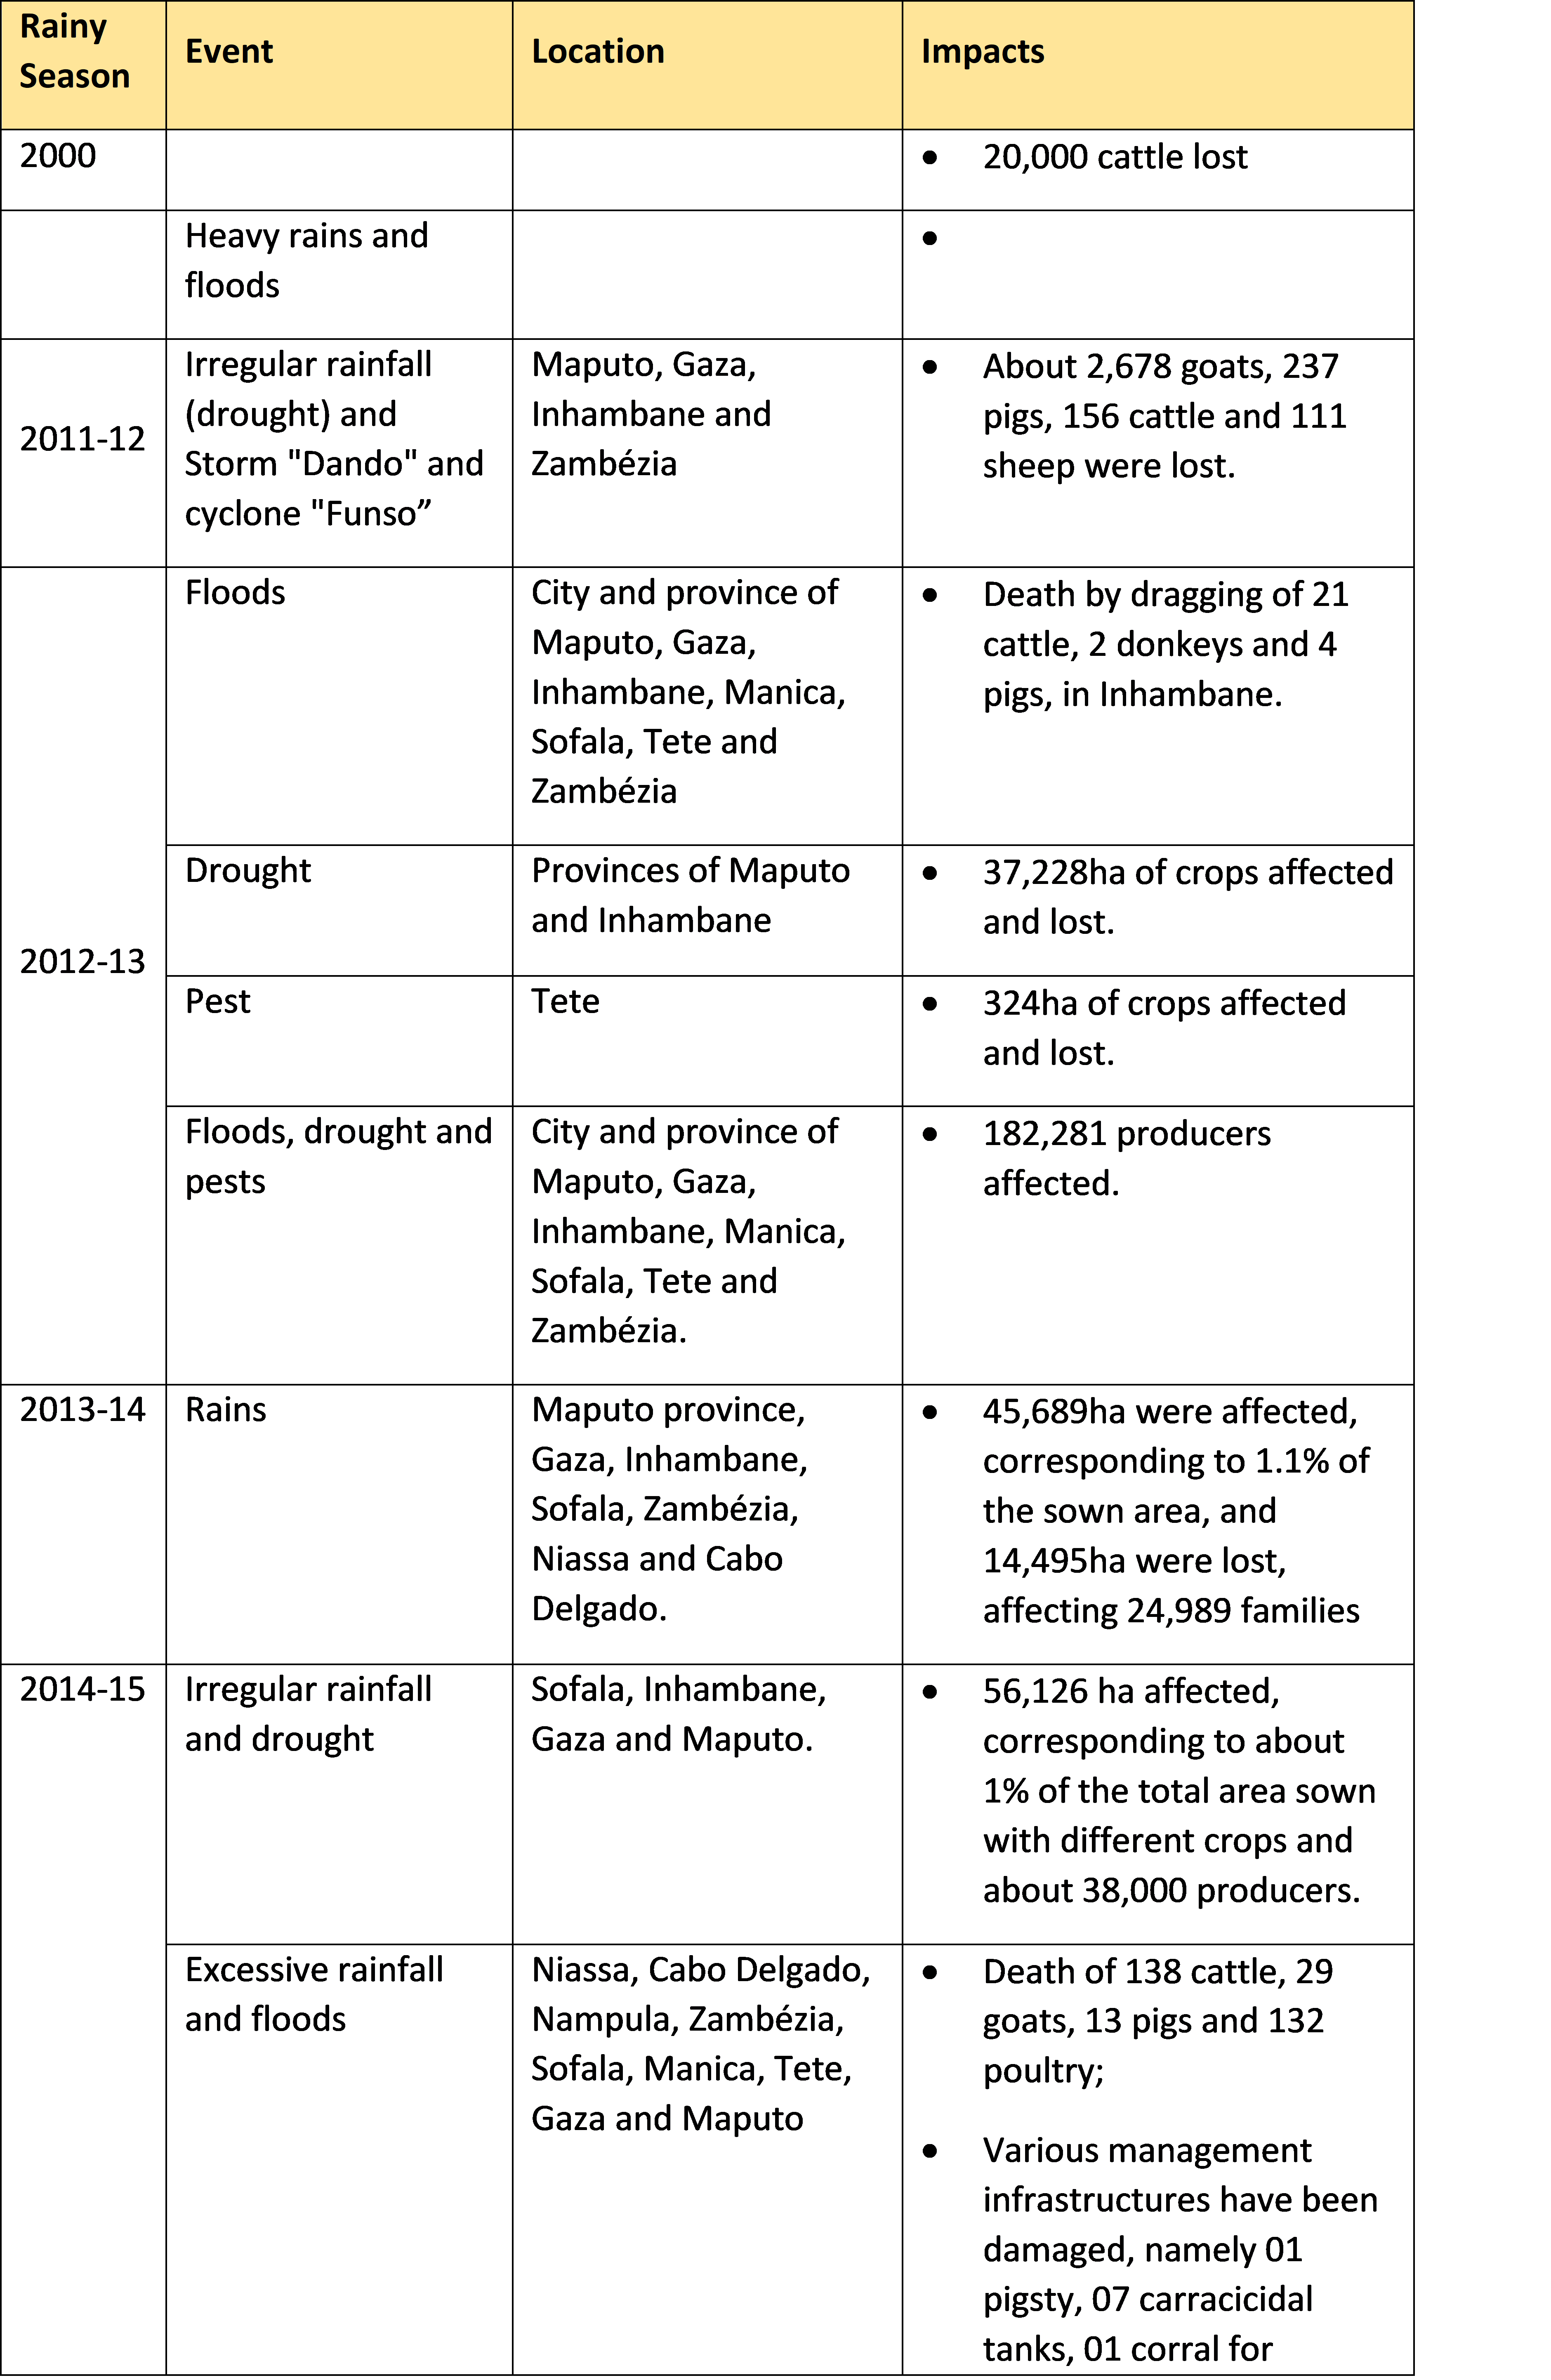
\includegraphics{Figure29.png}

\emph{(Source: Second National Communication Draft, p.~137-139; 144-146. Translated from Portuguese)}

\hypertarget{actions}{%
\subsection{Actions}\label{actions}}

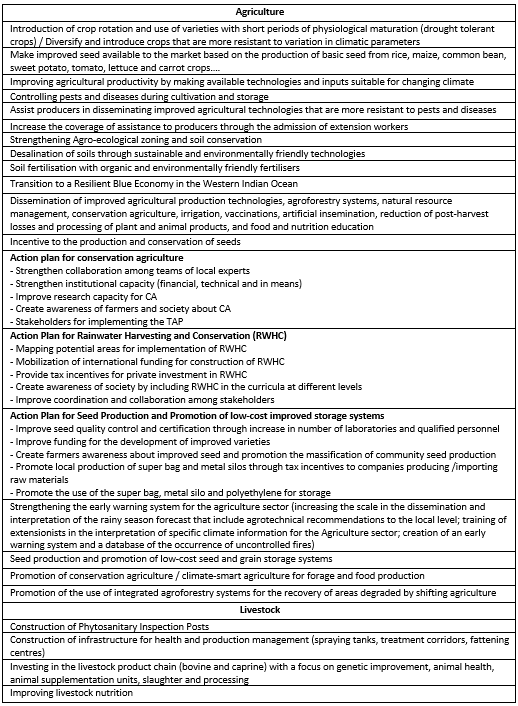
\includegraphics{Figure30.png}

\emph{(Source: NAP Prototype, 25.09.2021, Climate Change Adaptation Assessment)}

\hypertarget{fishery}{%
\section{Fishery}\label{fishery}}

\begin{itemize}
\tightlist
\item
  \textbf{Objective: Increase the resilience of fisheries}
\end{itemize}

\hypertarget{context-1}{%
\subsection{Context}\label{context-1}}

The Mozambican coastline has an extension of about 2,700 km, and several fishing resources can be identified. According to the Fisheries Master Plan (2010-2019), it is estimated that the potential of fishery products in Mozambique is around 332,000 tonnes, the main resources being shallow water shrimp (in the Sofala Bank and in the Maputo Bay), deep-sea crustaceans (in the continental slope of the central and southern zone), horse mackerel and mackerel (in the Sofala Bank) and demersal fish (in the southern and northern zone).

It is estimated that the fishing sector contributes about 4\% to GDP (MIMAIP, 2016) through the export of shrimp, prawns and other fishery products, with a global production of about 151,000 tons per year from fishing marine and inland waters (Ministerial Diploma No.~161/2014 of 1 October). Fisheries contribute to food security and especially by providing about 50\% of the animal protein consumed in the country (MIMAIP, 2016). Therefore, a breakdown in fisheries-based ecosystems and resources will have severe socio-economic implications.

\emph{(Source: Second National Communication Draft, p.~19. Translated from Portuguese)}

\hypertarget{vulnerability-to-climate-change-and-disasters-1}{%
\subsection{Vulnerability to Climate Change and Disasters}\label{vulnerability-to-climate-change-and-disasters-1}}

The fishing sector represents about 3\% of the country's GDP, resulting from the export of shrimp, prawns and other fishery products. On the other hand, fishing resources are the source of subsistence and income for around 60\% of the Mozambican population living in coastal areas. However, the IPCC (2007) indicates that coastal regions are the ones that will suffer the most from the impacts of climate change. For these reasons, it is important to determine the vulnerability of fisheries resources to climate change and identify adaptation mechanisms in order to achieve the sustainability objectives of the fishing activity.

Climate change risks to marine and fisheries resources include increases in temperature, precipitation and sea level, coastal storms and acidification of estuaries. This could decrease fish stocks, alter markets and influence tourism in the marine environment.

\emph{(Source: Second National Communication Draft, p.~19; 162. Translated from Portuguese)}

\hypertarget{actions-1}{%
\subsection{Actions}\label{actions-1}}

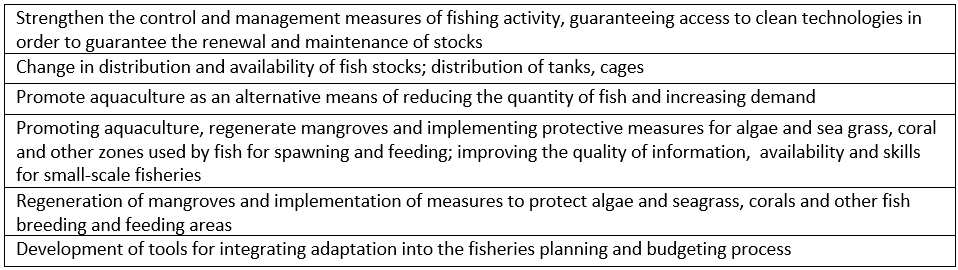
\includegraphics{Figure31.png}

\emph{(Source: NAP Prototype, 25.09.2021, Climate Change Adaptation Assessment)}

\hypertarget{food-security-and-nutrition}{%
\section{Food Security and Nutrition}\label{food-security-and-nutrition}}

\begin{itemize}
\tightlist
\item
  \textbf{Objective: Guarantee adequate levels of food security and nutrition}
\end{itemize}

\hypertarget{context-2}{%
\subsection{Context}\label{context-2}}

Food insecurity and chronic malnutrition are among the greatest development challenges for Mozambique. Chronic malnutrition affects 43\% of children under the age of five. In 2015, there were 2.1 million (out of 4.8 million) {[}7{]} children with chronic malnutrition. This situation is especially critical in children aged one to five years, 47\% of whom had short stature for their age (chronically malnourished) and 6.1\% suffered from marasmus (acute malnutrition). In addition, more than half of women (51\%) of reproductive age are anemic.

In Mozambique, malnutrition rates increase progressively from south to north. Chronic malnutrition is over 50\% in the north, in Nampula and Cabo Delgado provinces, while it is less than 30\% in Maputo and Gaza provinces.

At the same time, 7.8\% of children under five years old are overweight. The prevalence of overweight/obesity in women of reproductive age (BMI\textgreater25kg/m²) is 16.4\%. This situation is especially worrying in urban areas, where this prevalence is 27\%, while in rural areas it is 10.5\%. Obesity (BMI\textgreater30kg/m²) affects 4.2\% of women of reproductive age (15-49 years), and its incidence is higher in urban families, reaching 8.9\% of these, and lower in rural areas, with prevalence of 1.6\%.

The 2016 study, Cost of Hunger in Africa, reveals that in 2015, malnutrition cost Mozambique almost 11\% of its Gross Domestic Product (GDP) - the equivalent of US\$1.7 billion. The loss of potential productivity as a result of malnutrition-related mortality, morbidity and reduced cognitive development accounts for much of this cost. It is estimated that between 2011 and 2015 alone, 211,611 child deaths are directly associated with malnutrition, representing 25.6\% of child mortality.

\emph{(Source: Nutritionally Smart Agriculture in Mozambique, p.~02-03. Translated from Portuguese)}

The effects of food insecurity are even more severe when many families in the country are weakened by diseases such as HIV/AIDS and malaria. These families lack labor at crucial moments of agricultural activity, such as sowing, weeding and harvesting, with an adverse impact on the cultivated area and yields. These families are also victims of malnutrition. Nutritional status is also low, and the lack of production for sale means lack of availability of money for health care. Low agricultural yields coupled with low levels of use of modern inputs such as fertilizers, improved seeds, and lack of proper water management also contribute to chronic food insecurity. The presence of poor rural roads means that an effective response to food shortages by traders in other areas is difficult.

The above situation is reflected in the current situation of chronic malnutrition whose main immediate causes in Mozambique are inadequate nutrient intake, high levels of infection and early pregnancy. Diets are monotonous, with micronutrient deficiencies, affecting the majority of the population. Malaria and gastrointestinal parasites affect half the population. The same proportion among women is attended in prenatal consultations for having sexually transmitted diseases, in addition to half of them being pregnant as children. Only 40 percent of children under six months are exclusively breastfed. Underlying causes of chronic malnutrition are food insecurity (especially in limited access to and use of nutritious food), poverty and inadequate practices in relation to caring for adolescent girls, mothers and children, as well as insufficient access to health, water and to sanitation services. The basic causes of chronic malnutrition, in addition to poverty, include the low level of general and nutritional education, and gender inequality (the latter responsible for early marriages and pregnancies).

\emph{(Source: National Investment Plan of the Agricultural Sector - PNISA 2013-2017, p.~16-17. Translated from Portuguese)}

\hypertarget{vulnerability-to-climate-change-and-disasters-2}{%
\subsection{Vulnerability to Climate Change and Disasters}\label{vulnerability-to-climate-change-and-disasters-2}}

Mozambique is a country prone to climate impacts that further compromise food and nutrition security in some areas. Mozambique ranks third among African countries most exposed to various climate-related risks, suffering from cyclones, periodic droughts and floods, and related epidemics. For example, due to Cyclone Idai, which hit the country in March 2019, hundreds of rural communities suffered from food shortages and plunged into a nutritional crisis. Six weeks later, Cyclone Kenneth arrived in northern Mozambique.

\emph{(Source: Nutritionally Smart Agriculture in Mozambique, p.03. Translated from Portuguese)}

Part of the food insecurity in Mozambique results from sporadic food shortages caused by disasters. One of the largest disasters occurred in 2000 with dramatic effects on the food security situation. Torrential rains and cyclones systematically provoked flooding with the most serious effects for the provinces of Maputo, Gaza, Inhambane, Sofala and Manica causing devastation. In addition to people being displaced, and extensive material damage to public infrastructure such as schools, hospitals, water and electricity supply systems, road, rail and telecommunications networks, damages include crop losses, particularly food and livestock. Flood periods are followed by years of drought that affect a significant proportion of crops, leading many families to face severe food deficits.

However, in order to address the impact of natural disasters on food security, it is of utmost importance to ensure that the investments to be made and changes to be made in food production do not compromise the food and nutrition security of vulnerable groups and the progressive realisation of the human right to adequate food.

\emph{(Source: National Investment Plan of the Agricultural Sector - PNISA 2013-2017, p.~16. Translated from Portuguese)}

\hypertarget{actions-2}{%
\subsection{Actions}\label{actions-2}}

\hypertarget{water-resources}{%
\section{Water Resources}\label{water-resources}}

\begin{itemize}
\tightlist
\item
  \textbf{Objectives:}

  \begin{itemize}
  \tightlist
  \item
    \textbf{Increase capacity to manage water resources in critical basins of the country}
  \item
    \textbf{Increase access and capacity to capture, store, treat and distribute water in major settlements/farming areas}
  \end{itemize}
\end{itemize}

\hypertarget{context-3}{%
\subsection{Context}\label{context-3}}

Mozambique is located in the eastern part of Southern Africa, has a total area of approximately 801,590 km2 and 2,700 km of coastline. According to INE, the population is projected to be 25.53 million in 2015, of which 68\% live in rural areas and 32\% in urban areas. The country is administratively divided into 11 provinces (Niassa, Cabo- Delgado, Nampula, Zambézia, Tete, Manica, Sofala, Inhambane, Gaza, Maputo-Province and Maputo-City. In terms of operational water resources management Mozambique has 5 Regional Water Administrations, namely: Northern, Central-North, Zambezi, Central and Southern (figure 1).

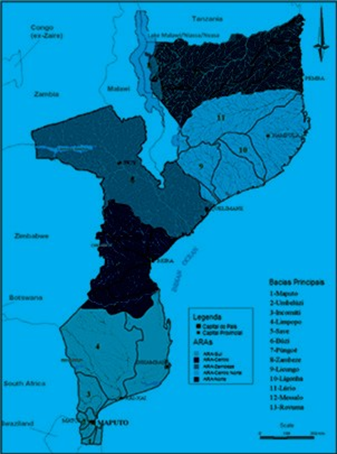
\includegraphics{Figure32.png}

\emph{Figure 1: Division of Mozambique by Hydrographic Regions}

The situation of water resources and their management in Mozambique can be defined as being at an intermediate stage of implementation of the sector reforms initiated at the beginning of the 1990s with the approval of Law No.~16/91 of 3 August 1991 approving the Water Law:

\begin{itemize}
\item
  The average availability of water resources can be considered as good, with an average annual runoff of 216,500 Mm3/year for a total population total population of 25.53 million inhabitants, which translates into an average of 8,481 m3/year of average per capita, which is well above the so-called water stress levels (\textless1,700 m3/year). However, its unequal distribution in space and time means that there are periods of the year and geographical locations of abundance and scarcity. The Centre-North and South regions are of greater concern because they have the lowest per capita availability;
\item
  Mozambique has one of the lowest storage capacities in Africa as it has the capacity to store only 0.5\% of its capacity of its average annual runoff. To make matters worse, 90\% of this capacity is concentrated in the Cahora-Bassa dam which has a main purpose of energy production. The country already faces storage challenges in meeting basic needs (water supply) in some of its main urban centres, namely Lichinga, Cuamba, Pemba, Nampula, Nacala, Quelimane, Beira/ Dondo and the Maputo metropolitan region;
\item
  The water bodies face some limited water quality challenges, mostly related to pollution due to irrigation returns and urban effluents upstream in neighbouring countries (in some of the shared basins) and due to mining activities, unregulated land uses in some watercourses and saline intrusion;
\item
  Mozambique is located downstream of all basins shared with other countries, except for the the Rovuma basin. In some of these basins intensive water use is already observed in the upstream countries, especially in agriculture. The Save basin presents the most critical situation due to the combination of seasonal rainfall and intensive use of upstream resources, where irrigated agriculture and a significant part of Zimbabwean industry is concentrated. The situation is not very different in the southern basins shared with South Africa and Swaziland with highly developed irrigated agriculture. Therefore, strategic planning for water resources management must take into account these adverse factors;
\item
  Due to its geographical location, Mozambique is highly vulnerable to the negative impacts of climate change that are projected to translate into increased occurrence of extreme events such as extreme floods and droughts and the occurrence of cyclones. The 2,700 km long coastline could suffer from rising sea levels with impacts on social and economic infrastructure and degradation of water quality, soil quality and biodiversity destruction in areas potentially affected by saline intrusion;
\item
  The monitoring of water resources is not yet at the desired levels and is characterised by a network of hydro-climatological observation network that does not meet some of the coverage requirements, the data collected is, in some cases, of poor quality and the monitoring, operation and maintenance costs are beyond the financial capacities of the management institutions;
\item
  The operational management of water resources is carried out in a decentralised manner by hydrographic regions of which there are five, namely North, Central North, Zambezi, Central and South. The process of establishing the respective institutions is still in the consolidation phase in terms of technical capacities and means, including the creation of some basin units and committees to complete the governance framework (River Basin Management Units and the respective Committees);
\item
  Strategic water resources development plans exist for only a small number of river basins;
\item
  Despite some progress observed with regard to the establishment of cooperation with neighbouring countries with which Mozambique shares hydrographic basins of Rovuma, Zambeze, Púngoè, Búzi, Save, Limpopo, Incomáti, Umbeluzi and Maputo, the process is still incomplete and needs consolidation;
\item
  The implementation of development projects and financing of day-to-day water management activities water resources is still dependent on government subsidies or funding from external cooperation partners, due to the limited amount of own revenue that the sub-sector produces; and
\item
  Existing institutional capacity (material and human resources) is still limited to respond adequately to the challenges of integrated water resources management at both central and regional/local levels.
\end{itemize}

\emph{(Source: Water Sector Action Plan for the Implementation of Sustainable Development Goals 2015 -- 2030, p.~1-3. Translated from Portuguese)}

\hypertarget{vulnerability-to-climate-change-and-disasters-3}{%
\subsection{Vulnerability to Climate Change and Disasters}\label{vulnerability-to-climate-change-and-disasters-3}}

Mozambique is located on the East African coast at the confluence of many international rivers and has 2,700 km of coastline. The country has a tropical and subtropical climate with some semi-arid regions in the south-western part. The average temperature tends to be high along the coast and lower in the interior, with a seasonal variation that includes cold and dry periods from April to September and hot and humid periods from October to March. Precipitation also shows the same trend, occurring in the hot season (November to April) and is not evenly distributed across regions, with the north recording averages of 150-300 mm and the south 50-150 mm per month in the wet season.

Mozambique is one of the African countries most vulnerable to climate change due to its geographical location described above, its climate specificities and also the fact that a significant part of the coastline is below sea level. Although more detailed models on climate change and its impacts are not yet available, some worrying trends have already been recorded and are projected to worsen in the future. Average annual temperature is estimated to have increased by 0.6°C from 1960 to 2006 (IRISH AID, 2016 \& MER, 2015), with highest increases observed in the southern region and according to various sources, the average temperature will continue to record significant increases in the future: IRISH AID (206) - from 1 to 2.8 ºC by 2060; MER (2015): up to 4.6 ºC by 2090/2100; Charles \& Twena (3006) - from 1.8 to 3.2 ºC by 2075; and INGC (2009) - average of 2.5 to 3.5 ºC by 2046/65. The frequency of hot days also registered an increase and is also projected to continue with the same trend with greater impact on the northern region. As for precipitation, no significant changes have been observed to date, except for the tendency to delay the onset of the rainy season and persistence of dry days and increase in the length of the dry season in some specific areas. Substantial changes in mean rainfall are also not expected in the future, but greater variability is projected with increased rainfall in the wet season offset by its decrease in the dry season and also increased rainfall on the coast relative to the interior (INGC, 2009 \& IRISH AID, 2016). The projected increase in precipitation for coastal areas is however less than the increase in evapotranspiration due to longer and more intense dry periods and reduced soil moisture.

Overall, projections suggest that the climate will become more extreme with intense droughts and floods and therefore affecting the availability of water resources in space and time impacting on the availability of water to meet basic needs, security of people and socio-economic infrastructure and food security in various forms, including:

\begin{itemize}
\item
  High levels of evapotranspiration could result in increased water demand in central and southern regions, which were projected to exceed the increase in precipitation on the coast;
\item
  Reductions in rainfall in the upstream countries of the international rivers that share watercourses with Mozambique that may potentiate a reduction in the availability of border flows, particularly in Zimbabwe and Zambia;
\item
  More accelerated reduction in per capita water availability due to reductions in water resources against population growth, especially in regions of higher population concentration;
\item
  The current pattern of water use combined with the impact of climate change will most likely to put considerable pressure on the Zambezi basin and place the Limpopo basin in absolute shortage;
\item
  The most direct social impact of reductions in water resource availability is the lack of water for basic needs, lack of water for irrigation, reduced groundwater recharge and reduction of the water table in major aquifers;
\item
  Negative impact on water quality and soil degradation as a result of saline intrusion in coastal areas.
\end{itemize}

The summary of the main impacts related to climate change as well as the strategic actions in the area of water resources that will contribute to the minimization of its impacts are presented in table 7.

\emph{Table 7: Climate change and potential impacts}

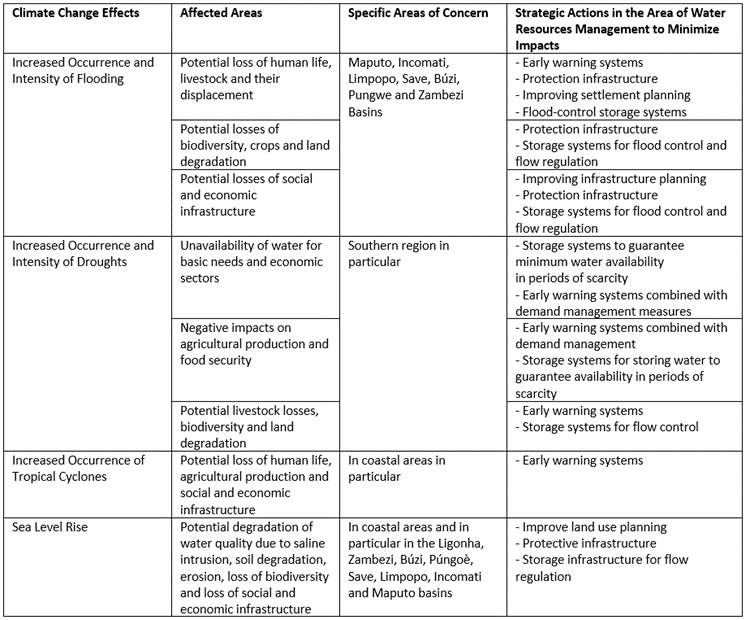
\includegraphics{Figure33.png}

Due to its geographical location, Mozambique is vulnerable to tropical cyclones and El Nino/La Nina phenomena that have been characterized by the occurrence of cyclical floods and droughts. Vulnerability to floods and droughts is exacerbated by the lack of hydraulic infrastructure capable of ensuring mitigation and enabling the country's resilience and adaptation to these events.

In recent years the country has frequently registered flood scenarios that have been having a negative impact on the country's socio-economic development (loss of human lives and socio-economic infrastructures). The main factors contributing to floods in Mozambique are: intense and concentrated precipitations in a certain period of time (rainy season), runoff from neighboring countries (9 basins shared with neighboring countries, almost all located upstream), watercourses crossing plains, human occupation of inundation and flood prone areas and the insufficiency of hydraulic infrastructures for flood mitigation. There are 10 flood prone basins, most of them being transboundary, and the most critical being the Zambezi and Limpopo, as shown in table 8, regarding the record of occurrence of critical floods in recent years.

\emph{Table 8: Historical flood records 1977 -- 2015}

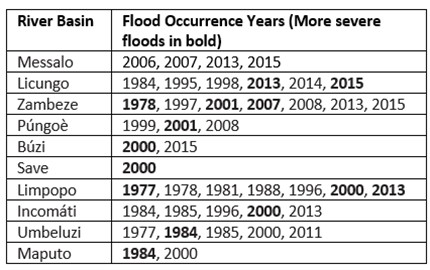
\includegraphics{Figure34.png}

Southern Mozambique, and particularly the provinces of Inhambane, Gaza and the northern part of Maputo province and the Central region with incidence on Tete province and southern Manica and Sofala provinces, present the highest vulnerability to droughts. The most severe droughts in recent years were registered in the years 1984/85, 1997/98 and 2015/2016 resulting in a negative impact on agricultural and livestock production and placing a considerable part of the population in a situation of extreme food insecurity.

Forecasts of the impacts of climate change available point to the worsening of droughts in the country and, above all, in the provinces of the southern region of the country.

\emph{(Source: Water Sector Action Plan for the Implementation of Sustainable Development Goals 2015 -- 2030, p.~8-11. Translated from Portuguese)}

\hypertarget{actions-3}{%
\subsection{Actions}\label{actions-3}}

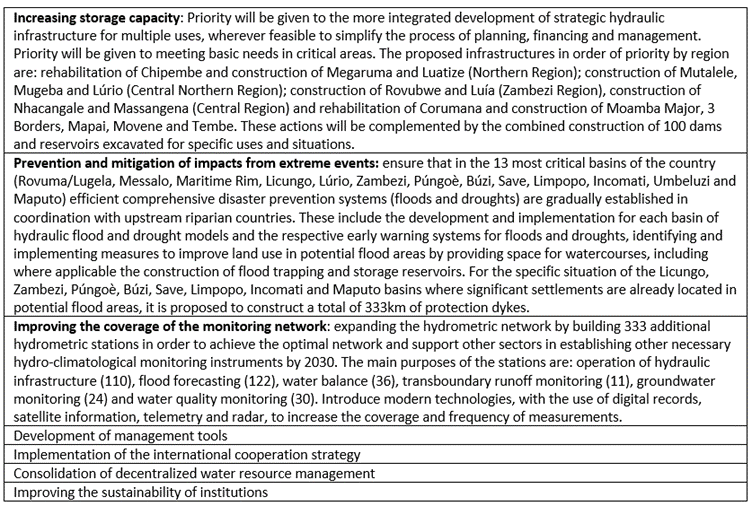
\includegraphics{Figure35.png}

\emph{(Source: Water Sector Action Plan for the Implementation of Sustainable Development Goals 2015 -- 2030, p.~4. Translated from Portuguese)}

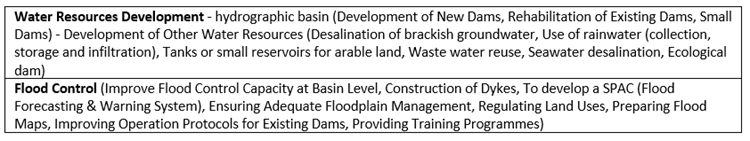
\includegraphics{Figure36.png}

\emph{(Source: National Water Resources Plan, p.~4-5;. Translated from Portuguese)}

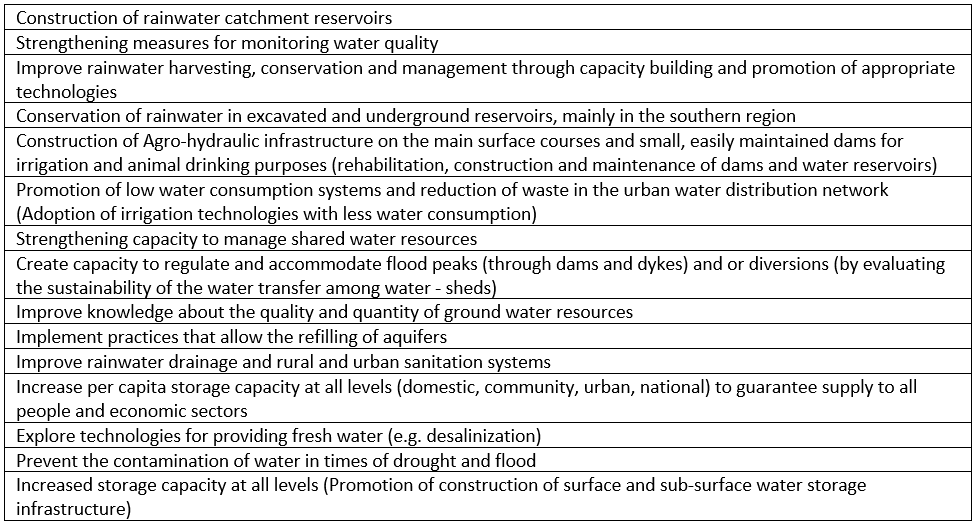
\includegraphics{Figure37.png}

\emph{(Source: NAP Prototype, 25.09.2021, Climate Change Adaptation Assessment)}

\hypertarget{health}{%
\section{Health}\label{health}}

\begin{itemize}
\tightlist
\item
  \textbf{Objectives:}

  \begin{itemize}
  \tightlist
  \item
    \textbf{Increase the resilience of health systems}
  \item
    \textbf{Reduce vulnerability to CC-related vector-borne diseases}
  \end{itemize}
\end{itemize}

\hypertarget{context-4}{%
\subsection{Context}\label{context-4}}

In Mozambique, health status indicators have progressed, but at different rates: Life expectancy at birth, although increasing from 42.3 in 1997 to 53.1 years in 2013 (INE), is still low compared to average African (55), denoting dissatisfaction of many basic human needs, such as adequate nutrition, clean water and sanitation, health services, etc.

Current data from Mozambique shows little progress in reducing maternal mortality and achieving universal access to reproductive health services. Despite the reduction registered between 1997 and 2003 (IDS - \emph{Demographic and Health Survey} - 1997 and 2003), in recent years the Maternal Mortality Ratio has been stationary (IDS 11) and is still unacceptably high (408/100.000 live births). Exposure to the risk of maternal death is also high, with overall fertility rates standing at 5.9 children, slightly higher than the previous IDSs, partly due to the low use of family planning (FP) services.

Child health indicators show remarkable and consistent progress in recent years. Under-5 and infant Mortality Rates (MT) decreased by more than 100\% between 1997 and 2011. However, the decrease in neonatal MT is occurring at a slower pace, requiring special attention in future strategies, having taking into account that about 81\% of these deaths occur during the first week of life and 32\% of them on the first day (National Study on Infant Mortality, 2009. MISAU).

Despite the slight reduction registered between 2003 and 2011, the prevalence of malnutrition in children under 5 years of age remains high. Given its direct and indirect effect on health as described below, the GRM launched in 2010 the Multisectoral Action Plan for the Reduction of Chronic Malnutrition in Mozambique 2011-2015 (2020).

The health status indicators presented above are largely influenced by the pattern of diseases and health problems. Indeed, the Burden of Disease in Mozambique is still dominated by communicable diseases, in particular HIV/AIDS, with an estimated national prevalence of 11.5\% (1.4 million infected) and Malaria with 3.2 million reported cases in 2012, which combined account for more than half of the deaths (27\% and 29\% respectively) in the general population. Diarrhoea, Respiratory Infections and Tuberculosis also contribute considerably to this profile. Under-five mortality shows the same pattern, but neonatal deaths, which contribute about 16\% of under-five deaths, are caused mainly by Prematurity (35\%), Asphyxia (24\%) and Neonatal Sepsis (17\%). It is also estimated that 30\% of under-five deaths have malnutrition as the underlying cause. Women of childbearing age, in addition to these common problems, face the additional burden of maternal deaths resulting from complications of pregnancy and childbirth: data from the National Neonatal and Maternal Health Needs Assessment (ANN-2007/2008) highlights uterine rupture (29\%), obstetric haemorrhage (24\%), puerperal sepsis (17\%) and postabortion complications as the main direct causes of maternal death, while the most frequent indirect causes include HIV/AIDS (54\%) and malaria (40\%). Moderate anaemia is also frequent among women aged 15-49 years (14\% in 2011).

The persistent occurrence of epidemic outbreaks adds to the burden of communicable diseases. There have been outbreaks of Cholera, between 2008 and 2010 (peak in 2009, with more than 19,000 cases), Measles, in 2010 (about 3,500 cases) and Meningitis, whose frequency and severity reflect a still limited responsiveness of the sector to these events. Other high incidence diseases are dysentery and other diarrhea.

Although the Neglected Tropical Diseases (NTDs) existing in Mozambique are not a direct cause of death, the high prevalence of trachoma, intestinal parasitosis (53\%), billiardsiasis (47\%), lymphatic filariasis (13\%), onchocerciasis, etc. in the country, which cause disabilities, delay the physical and mental development of children, and their correlation with anaemia and malnutrition, etc, contribute significantly to increase the burden of disease, especially on schoolchildren, in addition to the social stigma and limitation of productivity of people affected by these diseases, aggravating the correlation between disease and poverty.

Noncommunicable diseases (NCDs) are considered to be responsible for 80\% of all deaths and 60\% of all causes of disability occurring in developing countries, with important consequences for the consumption of health services as well as economic resources. These diseases and trauma are beginning to influence the epidemiological profile of the country and, consequently, the burden of disease and the pressure on health services. Among the NCDs, Cardiovascular Disease (CVD) is the most important cause of morbidity and mortality, the main risk factor being Arterial Hypertension (ATH). The prevalence of hypertension is estimated at 35\% nationally, being higher in cities (40.6\%) than in the countryside (29.8\%) and increasing with age. Diabetes is also a major cause of disease and premature death and is responsible for increased risk of CVD. In Mozambique, the prevalence of diabetes in the population aged over 20 years was 3.1\% in 2003, and was projected to increase to 3.6\% in 2005. Similarly, cancers are increasing their expression in the causes of consultation and hospitalization in the country: for example, the number of oncology outpatient consultations at Maputo Central Hospital (HCM) has increased by more than 50\% in the last 3 years, and the bed occupancy rate has exceeded 100\%. Data from the Pathological Anatomy Services (APS) of HCM for the periods 1991-2008 and 2009-2010 in Maputo City show that among women the most frequent cancers are cervical cancer (31\%), followed by breast cancer (10\%) and Kaposi's sarcoma (7\%). Among men, Kaposi's sarcoma (16\%), prostate cancer (16\%) and liver cancer (11\%) are the most common. Regarding trauma, data from the HCM Intensive Care Unit indicate that, in 2012, traffic accidents were the 3rd basic cause of death (10\%) and complications of trauma represented the 6th direct cause of death, in that service.

The health status and distribution of the burden of disease across the national territory (provinces and districts) and population groups are not uniform. People living in rural areas and on the outskirts of cities, who are also the poorest, as well as children and women, bear much of the brunt of the disease. The IDS 2011, e.g., states that fertility is much higher in rural areas than in urban areas (4.5 and 6.6, respectively); mortality in children under 5 years old in poor families was almost 2 times higher than that observed in richer families, in the IDS 2003; malnutrition in children is more pronounced in the northern provinces and in rural areas.

Several factors contribute to this pattern of disease, which are called, on the whole, ``social determinants of health''.

\textbf{Determinants of Health and Health Inequities}

The health status of individuals, communities and populations is not conditioned solely by genetic and biological processes, but also by the social and economic conditions in which people live. These social determinants of health include political, socio-cultural, economic, geographical factors and the environment which influence the onset of disease and access to and use of health services. However, these factors influence regions and population groups differently, resulting in inequities in the health status of individuals, communities and populations.

The \textbf{political context} has an enormous influence on the health of the population, since it must create the political-legal environment conducive to the promotion and preservation of the health of citizens, in compliance with the principle of equity. In Mozambique, a legal framework favourable to health and the pursuit of equity exists: at the supra-sectoral level, the Constitution of the Republic defines the Republic of Mozambique as a State of social justice; it defines the defence and promotion of human rights as one of the fundamental objectives of the state, guarantees protection for special groups such as children, the physically disabled, the elderly; establishes the principle of gender equality, assures all citizens the right to medical and health care and promotes equality in its access; the population policy (1999) recognises the existence of imbalances and inequalities in access to resources, infrastructures and social services, highlights the principle of respect for human rights and the right to equality and equity between men and women, and recognises the need to invest in areas that respond to the needs of a predominantly young population. It presents the reduction of the Maternal Mortality Rate (MMR) and of under-five mortality as one of its fundamental objectives; the Government's Five-Year Programmes and poverty reduction strategies place health at the top of the priorities. There are also several intersectoral policies and strategies (social action, education, agriculture, etc.) that highlight the role of health or attribute responsibilities to the sector. At the intra-sectoral level, sector policy documents and strategies emphasize GRM commitment to health promotion and preservation, as well as equity in access to and distribution of health resources and benefits. Similarly, there are policies that promote administration reforms, particularly decentralisation. In legal terms, the National Health Service (NHS) was created by law 25/91 and brings together only public institutions, namely US (Health Units), training and research institutions, laboratories, etc. Additional legislation frames the operation of the private for-profit and non-profit sector.

\textbf{Economic factors} are highly correlated with health outcomes: low income and low employment are unequivocally harmful to health. Despite constant economic growth in recent years, Mozambique is still among the poorest countries in the world, with an unequal distribution of wealth: about 54\% of Mozambicans live below the poverty line, especially in rural areas (56.9\%) and in the provinces of Zambézia (70\%), Maputo Province, Gaza, Sofala and Inhambane. It is in the poorest populations of these regions that the worst indicators of health status and consumption of health services are found, as evidenced by various studies: e.g.~the IDS 2011 shows that under five mortality in rural areas is 1.4 times higher than in urban areas; in Zambézia only 5\% of married women use some modern contraceptive method. According to INE (National Institute of Statistics - Statistics of Mozambique 2011), the structure of the Mozambican economy is dominated by Agriculture (15\%), Manufacturing (14\%), Transport and Communications (13\%) and Trade and Repair Services (12\%), which may determine the pattern of occupational diseases and/or lead to health problems resulting from the environmental impact of these economic activities.

The determining role of \textbf{malnutrition} in the genesis or worsening of disease and general health status is well known, particularly in women and children. The negative influence of malnutrition on children's physical and cognitive development, as well as on individual productivity and its consequent impact on the economy, is also well known. The immediate causes of chronic malnutrition are inadequate nutrient intake, high levels of infectious diseases and early pregnancy; underlying causes are food insecurity (especially limited access and use of nutritious food), poverty and inadequate practices regarding the care of adolescent girls, mothers and children, as well as insufficient access to health and water, especially in rural areas, where it affects 45.5\% of children (35\% urban), and with greater severity in the provinces of Nampula (55.3\%) and C. Delgado (52.7\%). About 69\% of children aged 6-59 months have anaemia, particularly in rural areas, a proportion of 72\% against 60\% of their urban counterpart, with the provinces of Cabo Delgado, Nampula and Zambézia (79\%) showing the highest proportions. About 54\% of women of reproductive age (15-49 years) have anaemia, also predominant in rural areas (55\%) and in Zambézia Province (62\%). These population groups and geographical areas also bear the greatest burden of infectious diseases and mortality rates.

\textbf{Agriculture} influences health in many ways: contributing to adequate nutrition through the provision of basic food items, or facilitating the spread of disease through contaminated food; by altering the environment (e.g., irrigation projects) it can create conditions for the spread of diseases such as malaria, billiardsiasis, etc. Agriculture is the livelihood base of many Mozambican families in rural and peri-urban areas, where the incidence and prevalence of disease and malnutrition is also higher. According to regular editions of the SETSAN InfoFlash (Technical Secretariat for Food and Nutritional Security - Information on Food and Nutritional Security in Mozambique), the country is characterized by the cyclical occurrence of pockets of Food and Nutritional Insecurity, sometimes extreme, affecting mainly the interior of the provinces of Gaza, Inhambane, Sofala, Manica and Tete, where the food is also not very diversified.

\textbf{Education}, especially for women, plays an important role in the health of the population, particularly children. Higher educated people have lower rates of morbidity from the most common acute and chronic illnesses, regardless of basic demographic and labor market factors. According to the 2007 Census, the illiteracy rate of women in Mozambique is still extremely high, at 64\%. The prevalence of chronic malnutrition in children of mothers with no education is almost double that of children whose mothers have secondary education or more (IDS 2011). The IDS also shows that 51\% of pregnant teenagers have no level of education, against 26\% of teenagers who have attained at least secondary education. Differences also appear in the use of health services: the degree of use grows with the increase in the user's educational level. For example, the percentage of births that take place in the Health Units is 40\% among women without any level of education, against 93\% among women with secondary education or more. On the other hand, health problems can undermine investments in education by, e.g., causing children to be absent or girls to drop out to take care of sick relatives.

According to the World Health Organization (WHO), 10\% of the global disease burden could be prevented by improving the availability of \textbf{clean water, sanitation, hygiene and water resources management}. Indeed, a large part of the occurrence of diseases such as diarrhea, malnutrition, malaria and neglected tropical diseases is attributable to the unavailability of clean water, inadequate sanitation or insufficient hygiene. According to the 2008 Multiple Indicators Survey (IIM), only 43\% of the population had access to safe water and 19\% to safe sanitation. The situation was most critical in rural areas where only 30\% of the population had access to safe drinking water and 6\% to adequate sanitation, compared to 70\% and 47\% in urban areas, respectively. The same study indicated that access to safe water was 6.5 times greater in the highest socioeconomic quintile compared to the lowest, with this difference being even greater in access to sanitation. It is in these poor areas that, e.g., frequent outbreaks of cholera occur.

The quality of \textbf{housing} and its basic conditions (water, sanitation and electricity) have a considerable influence on the health status of individuals and populations, as they can facilitate the spread of respiratory, skin and vector-borne diseases. In Mozambique, the precarious housing conditions in rural, peri-urban and even urban areas are well known. According to the 2007 census, around 70\% of households live in huts and with an average of 4.4 people per household, being highest in urban areas of Maputo and Sofala with 4.9 and 4.8, respectively. Overall, 85.4\% of private dwellings have 1-2 rooms for sleeping (rural: 90; urban 75\%), which, combined with the size of the households and the precarious housing conditions, denotes overcrowding and consequent facilitation of the spread of the above mentioned diseases. Additionally, only 10\% of homes are connected to the electricity grid and most of them use petroleum, paraffin, kerosene (54\%) and firewood (30\%) as a source of energy; only 10\% of households have piped water inside or outside the home, and most residents use unpiped water, mostly from unsafe sources (90\%). In terms of sanitation, around 53.7\% of households do not have a toilet/latrine, or have unimproved latrines (30.7\%). The impact of water and sanitation on health has already been described in the previous paragraph.

\textbf{Social-cultural factors} impact on health by influencing health exposure and vulnerability, risk behaviour, the effectiveness of health promotion efforts and the access, availability and quality of health care, as well as shaping perceptions and responses to health problems. Mozambique is a country of enormous cultural diversity with beliefs and taboos that negatively affect health: there are reports of religious sects refusing blood transfusion and/or vaccination in some provinces, beliefs about curing HIV that favour the spread of the disease, etc. Differences in gender-based and culturally constructed social relations, especially in access to resources, power or decision-making, and roles and responsibilities, have implications for the health status of the population, particularly of women who often see their decision-making capacity limited. This gender influence is exerted in various ways: exposure, risk and vulnerability; nature, severity or frequency of health problems; how symptoms are perceived; service-seeking behaviour; access to health services; ability to follow treatment; long-term social and health consequences, etc. In Mozambique, for example, polygamous behaviour increases the risk of women contracting HIV, the prevalence of which, according to INSIDA 2009, is much higher among women (13.1\%) than men (9.2\%). The 2003 IDS showed that under-five mortality rates are more pronounced in male children. The Strategy for Inclusion of Gender Equality in the Health Sector (2009) highlights the disrespect for women's sexual and reproductive rights, women's weak decision-making power over their own bodies and lack of decision to seek health services during pregnancy as important contributing factors to high maternal morbidity and mortality. Data from the 2011 IDS shows that chronic malnutrition is more prevalent among male children, which implies more serious long-term health consequences for this population group.

\textbf{Health services} are in themselves a determinant of health. Access to quality promotional, preventive and curative health care contributes to reducing morbidity and mortality and improving quality of life. In Mozambique, and despite the considerable improvements found in the 2008 Household Survey (IAF), especially in the northern rural areas, less than half of the families have access to a Health Unit in less than 45 minutes. The study reports that access has worsened in urban areas, possibly due to urbanization with greater population growth on the outskirts of cities, where access to public services is lower, and greater reliance on hospitals and other medical facilities in urban areas, which reduces demand for primary-level health unit. On the other hand, the IDS 2011 shows that only 54\% of births were attended by health professionals, noting a huge difference between urban (80\%) and rural (44\%) areas, and especially in Zambézia, which even , worsened from 2003 (32\%) to 2011 (26\%). Even with extension services provided through mobile brigades, coverage with full vaccination of children between 12-23 months of age is still 64\%, being higher in urban areas with 75\% and lower in rural areas (60\%), and Zambézia with the worst index.

Other health determinants that are beginning to dictate the worsening or emergence of diseases that will in the future change the epidemiological profile of the country, and put even more pressure on health services include working conditions, which influence the risk of accidents and occupational diseases, new habits of life that result in behaviours that are harmful to health, the potential effects of industrialisation on the health of workers and surrounding communities, the increase in road traffic and its consequences on accidents, air and noise pollution, physical activity, climate change (warming and natural disasters) which magnify NCDs and communicable diseases, among others. Long-term policies in the health sector and beyond must deepen analysis of these important determinants and begin to strengthen actions in these areas.

\emph{(Source: Strategic Plan for the Health Sector PESS 2014-2019, p.~8-15. Translated from Portuguese)}

\hypertarget{vulnerability-to-climate-change-and-disasters-4}{%
\subsection{Vulnerability to Climate Change and Disasters}\label{vulnerability-to-climate-change-and-disasters-4}}

Climate change is a global phenomenon and there is an urgent need to establish the relationship between it and health, as climate is one of the determinants of health and its change can exacerbate the health problems already affecting developing countries.

The resilience of the human population to climate change is related to water quality, environmental sanitation and food and nutrition security. According to the Intergovernmental Panel on Climate Change (IPCC 2014), most of the impacts of climate change in this sector in developing countries will be caused by malnutrition, malaria and diarrhoea, and could enable the worsening of cases of cholera, meningococcal meningitis, yellow fever, among others.

Mozambique is one of the countries that suffers the impact of climate change on health, resulting from extreme events (droughts, floods, tropical cyclones) that are increasingly frequent and intense. Climate change exacerbates diseases related to water, environmental sanitation, those spread by climate-dependent vectors, and malnutrition (USAID, 2018). However, the paucity of complete data on the relationship between climate and disease makes it difficult to quantify the potential impact of climate change on disease risk in the country (INGC, 2009).

Extreme weather events such as cyclones and floods are often associated with loss of life, socio-economic damage, isolation of communities, human suffering, loss of property, destruction of critical infrastructure (e.g.~health facilities, schools, access roads, etc.) and other indirect losses. Additionally, these events have other negative health consequences, e.g.~leaving health facilities without water, sanitation systems or power; blocking access routes to health facilities; interrupting the cold chain of vaccines, reagents and some medicines; destroying warehouses and depots of health consumables; causing delays and absenteeism of health personnel, etc.

Extreme weather-related events that occur frequently in Mozambique, such as tropical cyclones, floods and droughts, often cause epidemic outbreaks such as cholera, diarrhoea and malaria; bringing enormous challenges to the health sector. Ongoing climate change has a potential to increase vector-borne diseases, food insecurity, hunger and malnutrition. However, the combined effects of biophysical and socioeconomic drivers of human health and disease and the capacity required to manage and respond to these challenges are uncertain.

\emph{(Source: Second National Communication Draft, p.~186; 26. Translated from Portuguese)}

\hypertarget{actions-4}{%
\subsection{Actions}\label{actions-4}}

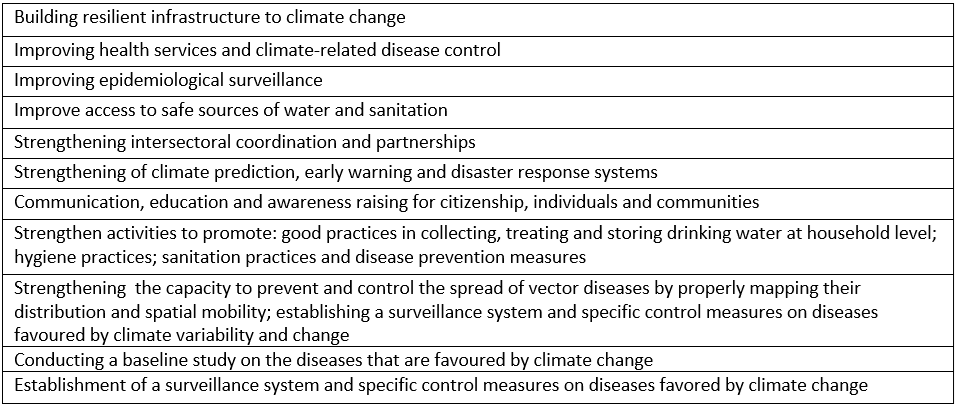
\includegraphics{Figure38.png}

\emph{(Source: NAP Prototype, 25.09.2021, Climate Change Adaptation Assessment)}

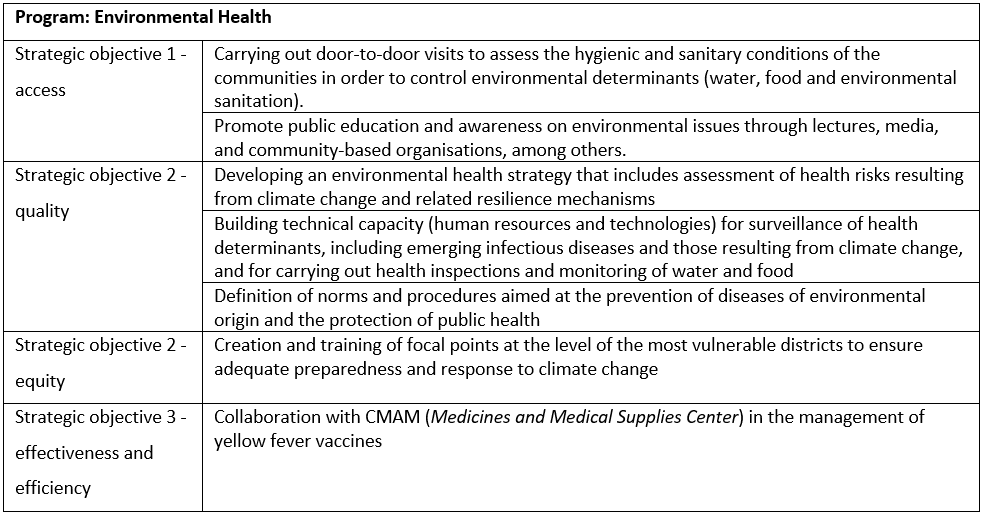
\includegraphics{Figure39.png}

\emph{(Source: Strategic Plan for the Health Sector PESS 2014-2019, p.~66. Translated from Portuguese)}

\hypertarget{energy}{%
\section{Energy}\label{energy}}

\begin{itemize}
\tightlist
\item
  \textbf{Objectives:}

  \begin{itemize}
  \tightlist
  \item
    \textbf{Expand climate resilient e-grid system to climate-proof agrarian ventures in 6 development corridors}
  \item
    \textbf{Increase energy efficiency}
  \item
    \textbf{Improve access to renewable energy}
  \end{itemize}
\end{itemize}

\hypertarget{context-5}{%
\subsection{Context}\label{context-5}}

The energy sector has experienced significant growth over the last two decades, both in terms of production and demand. Although consumption of modern energy sources has shown a remarkable evolution, particularly electricity and gas consumption, forest biomass continues to be the most important source of energy used in the country (ME, 2012). Indeed, it is estimated that about 77\% of Mozambican families depend on biomass, mainly charcoal and firewood, to meet their energy needs (Mahumane \& Mulder, 2016).

This reality is due to the fact that the majority of the population in rural areas (estimated at around 70\%) resorts to the use of firewood to meet their cooking and water heating needs, while in urban areas, whose population numbers have been growing at a rapid pace, they use charcoal for cooking, despite the growing rise in the price of this form of energy, and the negative impacts associated with it. It should be noted that, according to the preliminary results of the latest census conducted by the National Statistics Institute, the urban population represents approximately 32\% of the country's total (INE, 2018).

\textbf{Electricity}

In terms of electricity production, it should be noted that Mozambique has a generation capacity much higher than its domestic consumption. The Cahora Bassa Hydroelectric Power Plant (HCB), with an installed capacity of 2,075 MW, is the main source of electricity generation in the country. Of the total capacity of HCB, 500 MW is dedicated to the country, consisting of 300 MW of firm energy and 200 MW of non-firm energy. The rest of the capacity, around 1,500 MW, is destined for export to South Africa. The total capacity for national consumption is 1,045 MW, which represents the sum of the capacity allocated by HCB (500 MW) and other generation plants , while the total capacity for export to neighboring countries is 1,860 MW, which is the sum of the HCB capacity for export and that of other emerging sources, natural gas (ALER, 2017). Regarding the electricity generation mix, 90\% is from hydroelectric sources, with the remaining 10\% coming mainly from natural gas. Figure 1.12, taken from the most recent strategy of the company Electricidade de Moçambique, illustrates the projection of the country's supply and demand; according to the firm, paradoxically, it is expected that the country will face an energy deficit around the year 2020 and that, according to the Integrated Master Plan for energy production, after 2021 there will be a surplus of electricity production that could be traded at competitive prices in the regional market (EDM, 2018).

A recent study on the renewable energy potential in Mozambique (Renewable Energy Atlas, 2014) indicates that the country has a huge potential for energy production, with an estimated capacity of about 23,000 GW of solar resources, followed by hydroelectric sources with 19 GW, wind potential with 5 GW and biomass resources estimated at 2 GW. From this potential, the government has identified priority projects for the exploitation of these resources, locally, including the possibility of injecting the energy generated into the national grid. In this context, the priority projects identified comprise the production capacity of 5,645 MW for hydroelectric sources, 600 MW for solar, 1,146 MW for wind, 128 MW for biomass and 20 MW for geothermal energy. The Atlas also highlights the need for adequate financing schemes for the effective implementation of these projects. Access to renewable energy represents an important contribution, especially for the socio-economic development of communities that are far from the national electricity distribution grid, as well as in mitigating climate change through the sustainable use of biomass resources.

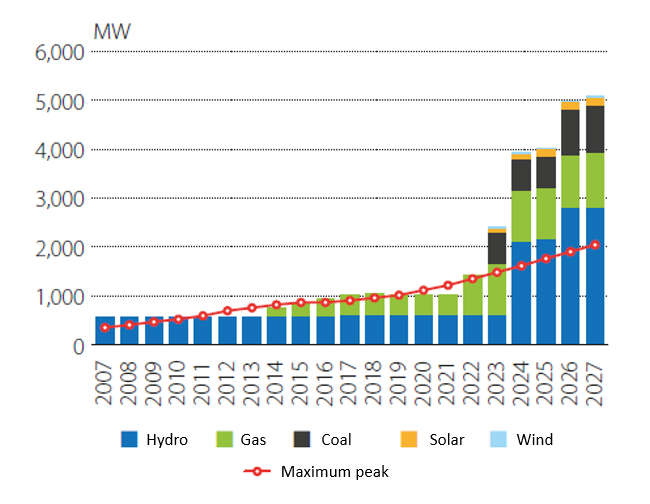
\includegraphics{Figure40.png}

Despite the remarkable efforts that have been carried out by Electricidade de Moçambique, in the field of electrification of the country, with an average of about 120 thousand new connections made per year in the last 15 years, according to the recent statistics available, the current coverage is only 25.9\% (EDM, 2015). In fact, this is the average rate of access to electricity, so it varies for each province, with the lowest rate in Cabo Delgado, Niassa and Zambézia provinces, with about 12\% each and, the highest, in Maputo City, with a level of 92\% (MIREME, 2018). The high level of dependence on biomass resources for energy purposes has serious implications on the health of the population and the environment. On the other hand, the current electrification rate represents a huge challenge for the achievement of the Sustainable Development Goals (SDGs), particularly the seventh goal, according to which ``by 2030, universal, reliable, modern and affordable access to energy services should be ensured'' (UN, 2015).

\textbf{Oil and Gas}

The consumption of liquid fuels grew at an average rate of 6\% per year, and from 2009 reached a growth rate of 15\% per year, on average. The transport sector is responsible for the largest portion of this increase, followed by the industrial sector. Consumption of petroleum products almost doubled in the period 2000 - 2011. Natural gas production in Mozambique has grown by an average of 5.3\% per year since 2006. About 95\% of the natural gas produced is exported to South Africa.

In the last decade, the energy sector has continued to grow significantly. With the increase in the exploration and consumption of natural gas in the country, new players have emerged, especially from the private sector, in the area of electricity generation, the independent power producers (IPP's) that have been expanding the national production capacity that currently stands at 2,724 MW (EDM, 2018).

The approval of the Natural Gas Master Plan, by the Government, in 2014, aiming at the massification of the natural gas produced in the country, has boosted the increasing use of this resource, not only in the production of electricity, but also in the industrial sectors, services and road transport, although at still low levels. Natural gas also represents an opportunity to diversify the mix of energy forms used in Mozambique, making an important contribution to industrial and socio-economic development. In turn, the consumption of liquid fuels, diesel and gasoline has doubled, mainly due to the increase in the national car fleet which, with 287.951 vehicles in 2010, almost tripled in less than ten years to 782,757 vehicles in 2018 (INE, 2011 \& 2018). It should be noted that part of these fuels is used in the extractive industry, which is an emerging sector with significant growth, and in electricity generation.

\emph{(Source: Second National Communication Draft, p.~20-22. Translated from Portuguese)}

\hypertarget{vulnerability-to-climate-change-and-disasters-5}{%
\subsection{Vulnerability to Climate Change and Disasters}\label{vulnerability-to-climate-change-and-disasters-5}}

Mozambique has enormous energy resources that are still unexplored, including coal and natural gas, water potential, renewable resources such as solar, wind, water, geothermal, ocean and forest and agricultural biomass sources (ME, 2011). At the same time, the country is one of the countries with the lowest levels of energy consumption in Southern Africa, with around 80\% of the country's energy consumption based on biomass (firewood and charcoal) and around 17\% of the population with access to electricity (ME, 2011).

Access to energy is a \emph{sine qua non} condition in the fight against poverty, as it is a means that intervenes in all key sectors of development, whether water, health, food refrigeration, lighting, and domestic heating, transport, agriculture, industrial production or even modern means of communication (Sebastião, 2013). In order to realize one of the national development objectives, the President of the Republic launched in November 2018 the Programme ``Energy for All by 2030''. This Programme aims to intensify access to electricity for more households and businesses nationally, as a contribution to Mozambique's universal electrification by 2030, defined in the National Electrification Strategy (ENE), approved by the Council of Ministers on 16 October 2018. The Project will support the expansion of power access to peri-urban and rural areas across the country by leveraging and extending the existing national electricity grid and deploying mini-grids on the basis of solar generation in areas not covered by the national grid.

INGD's rainy season balance reports show that the power sector has been affected by extreme events that occur in the country, particularly strong winds, tropical cyclones, floods and inundations (Table 3.13).

\emph{Table 3.13: Impacts of extreme events on the energy sector}

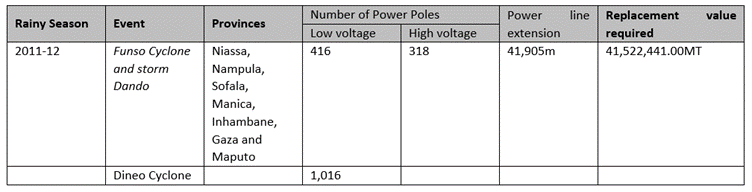
\includegraphics{Figure41.png}

Extreme weather events have resulted in the destruction of privately and publicly owned solar panels. One of the examples is the destruction of 11 solar panels providing electricity to a health house in Mossuril district, Nampula province, during the passage of cyclone Jokwe in Mossuril district.

\emph{(Source: Second National Communication Draft, p.~185-186. Translated from Portuguese)}

\hypertarget{actions-5}{%
\subsection{Actions}\label{actions-5}}

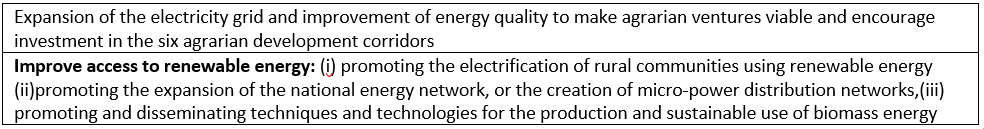
\includegraphics{Figure42.png}

\emph{(Source: NAP Prototype, 25.09.2021, Climate Change Adaptation Assessment)}

\hypertarget{infrastructure}{%
\section{Infrastructure}\label{infrastructure}}

\begin{itemize}
\tightlist
\item
  \textbf{Objective: Sustainable landscape planning and management to ensure climate resilience}
\end{itemize}

\hypertarget{context-6}{%
\subsection{Context}\label{context-6}}

The establishment of infrastructure in Mozambique is a process that has evolved throughout the country's history. Soon after independence in 1975, the infrastructures that existed at that time underwent an evolution that accompanied the country's socio-economic development.

In line with the National Development Strategy (2015-2035), the construction sector will be boosted by the construction of logistics infrastructure for large projects in the area of natural resources, infrastructure in the area of electricity, water and transport and projects of construction of houses for housing.

Next, the main existing infrastructures in Mozambique, their functionality, and the role they have played in the context of CC will be described.

\textbf{Road Network (Roads and Railways)}

In Mozambique, the road network is managed by the National Roads Administration (ANE) created by Decree 15/99 of 27 April 1999, as a public institution with legal personality and administrative and financial autonomy, under the supervision of the MOPHRH. In the structuring of ANE, the road network in Mozambique is classified as (i) primary (5,971 km); (ii) secondary (4,915 km); tertiary (12,603 km); and (iv) vicinal (6,567 km). Within this road network, the National Road No.~1 stands out. It runs longitudinally along the national territory in a north-south direction with a length of approximately 2,500 km. The road network in Mozambique provides overland connections to all cities and district headquarters of the country, in addition to other points of great importance.

From the perspective of transporting goods, the road network is supported and complemented by the rail and port system, which is managed by the Ports and Railways of Mozambique (CFM). The railway and port system has a network of approximately 2,983 km of railway line divided by a total of eight lines; three in the south zone, two in the central zone and three in the north zone. The rail network connects the three main ports in Mozambique (Port of Maputo, Port of Beira and Port of Nacala) to terminals located inland. Thus, the southern area of Mozambique has the Ressano Garcia Line, Goba Line, and Limpopo Line, which depart from the Port of Maputo to South Africa, Swaziland and Zimbabwe respectively. In the central area, the railway network includes the Machipanda line that links the port of Beira to Zimbabwe, and the Sena line that departs from Dondo to the city of Chipata in Zambia. In the northern zone, the railway network has the Nacala-Cuamba Line, which departs from the Port of Nacala to the City of Cuamba, and two lines that connect two cities; the Cuamba-Lichinga and Cuamba Entre-Lagos Line.

The 2018 PES prioritizes the development of socio-economic infrastructure, in this particular case by the rehabilitation of roads (the expectation is to rehabilitate 175km of national and regional roads, having been possible 137km equivalent to 78\%; a plan of 95km of asphalting of National and Regional roads, having been possible 44km equivalent to 46\%; regarding construction, rehabilitation and maintenance of bridges, the plan was to cover 15 of them, having been possible 18 bridges, equivalent to 120\% for first Semester 2018). At the same time, the ports represent a cargo gateway to the country and to the Austral Region, considering the many large ships that dock there.

\textbf{Port and Airport Network}

Mozambique, being a coastal country has the privilege to have conditions for maritime navigation and therefore has a port network of great importance not only for the country but also for the Southern African region. The largest ports in Mozambique (Maputo Port, Beira Port and Nacala Port) are particularly connected to the railway network, which guarantees the handling and transport of heavy cargo to the hinterland countries. In addition to the rail link, the ports are connected to the road network which makes a good system for handling and loading cargo.

The Airports are also a gateway for passengers and cargo both from outside and inside the country. The country has an airport network consisting of eleven airports distributed throughout the country, and located in the cities of Maputo, Inhambane, Vilanculos, Beira, Chimoio, Quelimane, Nampula, Nacala, Tete, Pemba and Lichinga. Of these, Maputo International Airport, Vilanculos Aerodrome and Beira Airport receive international flights. Similarly to the Ports, the airports are connected to the road network which in turn guarantees the integrated transportation of people and goods at a national level.

\textbf{Telecommunications and Electricity Infrastructures}

The backbone of the telecommunications and electrical network in Mozambique is somewhat robust. The network was built since the 1980s, and followed the transformation story of the Mozambican telecommunications company, formerly known as Correios Telégrafos e Telefontes (CTT) (Posts, Telegraphs and Telephones) until 1981, when it became known as Empresa Nacional de Telecomunicações (National Telecommunications Company) - state-owned company, in 1992, became known as Telecomunicações de Moçambique (Mozambique Telecommunications), and in2019 it merged with Mozambican mobile telephony, renamed Mozambique Telecom (Tmcel). During the evolution of the telecommunications company, several infrastructures were built, with an emphasis on fiber optics, part of which crossing the underwater part and another on the continent that connects practically all the provinces of Mozambique, including the main cities. In addition to fiber optics, Tmcel currently has a network of towers across the country, and stations with different communication equipment. There is also a network of other mobile phone companies and radio and television stations that use specific equipment that is often exposed, or in places at risk from CC.

The electricity grid in Mozambique is managed by Electricidade de Moçambique EDM (Mozambique Electricity), which operates the public service of generation, transmission, distribution and sale of electricity throughout the country. For the exercise of its activities, EDM has a series of infrastructures, ranging from power generation stations, transmission lines, energy transformation substations, among other infrastructures spread throughout the country.

\textbf{Education and Health Infrastructure}

The Education System in Mozambique has a network of infrastructures dedicated to the teaching process. Of these infrastructures, the network of primary, secondary and pre-university schools spread across the country stands out. Higher education infrastructures are also dispersed throughout the country, but these are preferably distributed at the level of the main cities in the country and at the level of the district capitals.

According to the Final Report of the Inventory of Infrastructure, Equipment, Human Resources, and Health Services (SARA-2018), in 2017 the country had a total of 1,625 public health units, of which 96\% provided primary health care in the 11 provinces of Mozambique and in 157 districts, being present in practically all districts of the country.

The GoM's effort to guarantee the right to Education and Health for the entire Mozambican population brings challenges for building infrastructure and allocating Human Resources, particularly in the more remote areas of the country. The challenge also extends to the allocation of health equipment to health units, and to the equipment of classrooms with desks and teaching materials. Some of the school infrastructure is still made of precarious material that is very susceptible to the impact of bad weather. On the other hand, even though it is advisable to build these infrastructures in ``safe'' locations, there are scenarios throughout the country where this choice is minimal considering the need to make these services available close to the populations. However, the Government's effort has always been to build infrastructures with high standards, capable of resisting the impact of bad weather. This effort has led to the use of some school infrastructures as shelter options to temporarily accommodate populations living in homes vulnerable to the impacts of extreme events.

\textbf{Housing Infrastructure and others}

The housing infrastructure in Mozambique is under the responsibility of the MOPHRH, which, through the Housing Promotion Fund (FFH), promotes access to decent housing, ensuring safety, durability, aesthetics, comfort and healthiness. The FFH has directed its efforts particularly towards young people and State Employees and Agents, in coordination with the different segments of society. Within the scope of its activities, from 2011 to 2018, the FFH has built nearly 4,000 houses and infrastructed nearly 13,000 plots in the different provinces of the country. This number of infrastructures is still far from satisfactory for the demand for housing in the country.

Despite the GoM's effort to have a regular and well-planned subdivision, the growing pressure for housing demand, especially in urban areas, constitutes a major challenge for the issue of land use planning. With population growth, combined with the trend of migration from rural areas to the city, the demand for housing surpassed the capacity of municipalities to provide sufficient plots for this demand, and to control the quality of residential infrastructure to be built. Another problem associated with the quality of residential infrastructure is the cost of building conventional houses, which in many cases is higher than the population's income. Thus, the main trend verified in the country was an increase in the use of land for the construction of residences and other infrastructure in peri-urban areas. For rural areas, populations prefer to settle in places close to district headquarters and administrative posts, water courses, roads and the coast, which also, in combination, contributes to a weak territorial ordering.

Informal settlements in the large cities of Mozambique bring environmental problems with them. Accelerated erosion and flooding are seen as the result of pressure on urban land use, which contributes to the increase of factors to be considered in the impacts caused by CC. Thus, over the last few years, more and more areas at risk of flooding and erosion have emerged in large cities. These locations are properly mapped and signposted to avoid setting up residences in these locations.

\emph{(Source: Second National Communication Draft, p.~190-195. Translated from Portuguese)}

\hypertarget{vulnerability-to-climate-change-and-disasters-6}{%
\subsection{Vulnerability to Climate Change and Disasters}\label{vulnerability-to-climate-change-and-disasters-6}}

The infrastructure network at the country level is one of the main platforms for economic development. These include the road network, port, airport, hospital, school, communication platforms, electricity generation and transport, among others. Infrastructure in general is essential for a country to function and for everyday life. A particular relevance of the infrastructure sector is the fact that they significantly contribute to a country's adaptive capacity in the context of CC impacts. In situations of extreme weather events, such as cyclones, most attention in Mozambique has been turned to infrastructure, considering that these constitute the means by which most rescue operations will take place. Thus, any interruptions in the infrastructure systems programmed for these operations imply a re-dimensioning of the strategy to rescue, or deliver food, medical and drug aid to the affected communities. In order to understand and minimize this effect, we highlight some initiatives taken by UN-Habitat and by the USAID Coastal Cities Adaptation Project (CCAP) in collaboration with district governments and municipalities, which carried out actions to develop house models resilient to weather events, and in raising awareness and training for the need to map critical infrastructure. The purpose of identifying and mapping these infrastructures is to identify, recognize and, if possible, predict their degree of resilience in the face of expected extreme events. The criticality of infrastructure lies in the fact that part of these are impacted by extreme events such as cyclones and floods, and negatively affect rescue activities.

The combination of road and rail network is preferred and practical for transporting goods. In the disaster risk reduction agenda, INGD and partners have used these routes for the transportation of material needed for prevention and mitigation. On the other hand, the GoM relies on these same infrastructures as means for rescue in the event of a disaster. With regard to the impacts of CC, the road infrastructure sector has almost always suffered heavy damage. Cyclically, several kilometers of roads are flooded and removed by the rainwater simultaneously with the soil. With the increase in river flows, several bridges and culverts have been damaged, resulting in the interruption of road traffic. Railroad infrastructures, although more resistant to the impacts of bad weather than roads, have also been affected, causing interruption in rail transport.

The port and airport network in Mozambique plays an important role in managing disaster risk caused by climate change, and appears as critical infrastructure in the same context. Throughout the history of climate events in the country, particularly in situations of intense rains and floods, airport positions have been activated as arrival points for humanitarian aid to the affected people as well as in search and rescue actions, taking into account that some roadways have been limited to transitability, including for providing access to disaster-affected places.

Communication and electricity infrastructures are part of the list of critical infrastructures in the context of CC, taking into account that these are essential for rescue and salvage operations. The criticality of this type of infrastructure calls for the need to redouble efforts by the GoM to ensure that they are increasingly resilient to bad weather. Over the past few years, communication and electricity infrastructures have been affected by extreme events, especially cyclones, in which strong winds have cyclically destroyed the equipment. As mentioned above, the destruction of equipment brings losses not only because of the damage, but also because their destruction negatively affects the operation of essential activities in the context of rescue and humanitarian assistance to victims.

As with other sectors, the school and hospital infrastructure sector is very susceptible to extreme events such as cyclones, heavy rains and floods.

Recent projections indicate that due to the impact of climate change, there will be an increase in the frequency, intensity and magnitude of disasters, and if there is no investment in resilience, annual losses could reach 450 million dollars by 2040, due to damage to agriculture, infrastructure and energy production.

The infrastructure sector is one of the most impacted by Climate Change, particularly in extreme events such as cyclones and floods. In each rainy season, there is always a negative balance in the different types of infrastructure in Mozambique. Thus, during the period under review, several infrastructures were destroyed by these events. In 2007, when Cyclone Favio passed through the Coastal Districts of the Province of Inhambane, around 80\% of the infrastructure in the District of Vilankulo was damaged, including residences and tourist establishments. The destruction caused by this cyclone spread to other districts, damaging around 130,000 homes and around 130 schools. In 2008, Cyclone Jokwe affected Nampula Province, destroying 9,316 houses and damaging around 3,220 houses. Cyclone Funso affected the country with strong winds, affecting more the provinces of Zambézia, which had a record of 12 deaths, seven of which occurred in the district of Maganja da Costa, where 1,610 houses were destroyed and one death occurred in the capital city of Quelimane, with heavy rains that flooded most of the neighborhoods due to poor drainage systems. In the city, floods destroyed 4 houses and several other towns along the coast suffered flooding. In Nicoadala district, the storm destroyed 66 homes.

\emph{(Source: Second National Communication Draft, p.~190-196. Translated from Portuguese)}

\hypertarget{actions-6}{%
\subsection{Actions}\label{actions-6}}

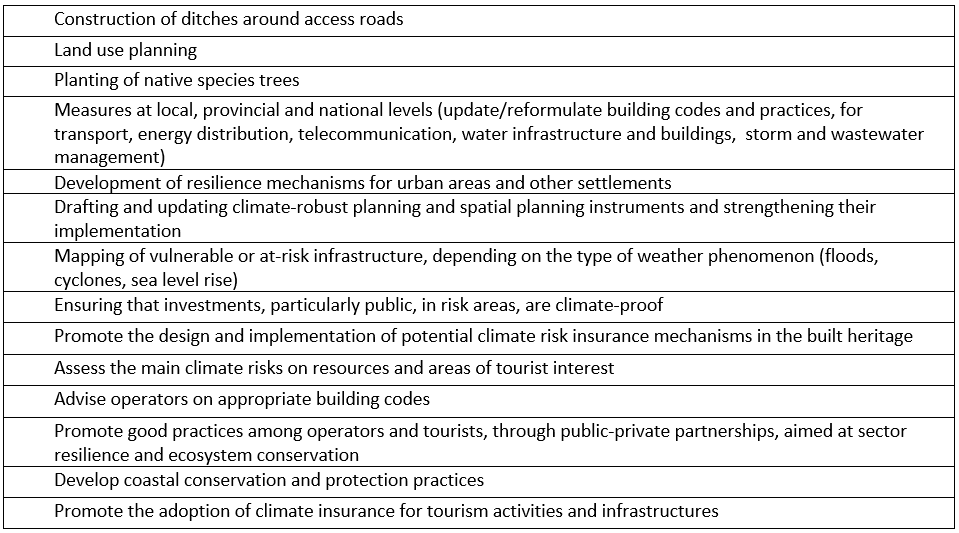
\includegraphics{Figure43.png}

\emph{(Source: NAP Prototype, 25.09.2021, Climate Change Adaptation Assessment)}

\hypertarget{coastal-zones}{%
\section{Coastal Zones}\label{coastal-zones}}

\hypertarget{biodiversity}{%
\section{Biodiversity}\label{biodiversity}}

\hypertarget{disaster-risk-human-safety-and-wellbeing}{%
\section{Disaster risk: human safety and wellbeing}\label{disaster-risk-human-safety-and-wellbeing}}

\hypertarget{social-protection}{%
\section{Social Protection}\label{social-protection}}

\hypertarget{cross-cutting-issues}{%
\chapter{Cross-cutting issues}\label{cross-cutting-issues}}

\hypertarget{mainstreaming-of-climate-change-adaptation}{%
\section{Mainstreaming of climate change adaptation}\label{mainstreaming-of-climate-change-adaptation}}

\hypertarget{gender-issues-lcip-vulnerable-groups}{%
\section{Gender issues / LCIP / Vulnerable groups}\label{gender-issues-lcip-vulnerable-groups}}

\hypertarget{gender-issues}{%
\subsection{Gender Issues}\label{gender-issues}}

The geographic distribution of the population of Mozambique is uneven and most are concentrated in the provinces of Nampula and Zambézia, with almost 40\% of the total population. Maputo City, Gaza and Niassa have the lowest rates of the total population, with less than 6\% each1 . This population is mostly young as a result of high fertility and mortality, which means that half of the population is under 15 years old. In the UNDP Human Development Index Mozambique is ranked 180th out of a total of 188 and is ranked 135th out of a total of 155 on the UNDP Gender Inequality Index (2015).

Furthermore, in the Gender Inequality Index, where inequality is analysed in three dimensions: a) reproductive health, b) empowerment and c) economic activities, it can be seen that in addition to the high maternal mortality rate and the occurrence of early pregnancies, women are at a greater disadvantage than men, especially in secondary education. The data on economic activities also show that in Mozambique structural inequality affects relations between men and women to a greater extent, since women work more than men and earn less than they produce.

\emph{Table 1: Gender Inequality Index}

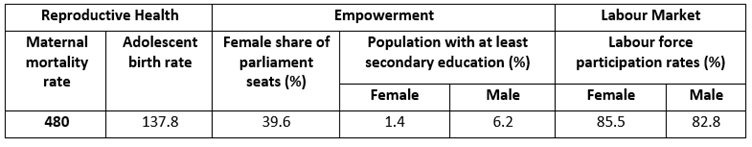
\includegraphics{Figure44.png}

\emph{Source: UNDP Human Development Report, 2015, p.~6.}

Regarding the Gender Development Index, as the table below shows, with the exception of life expectancy at birth, for all other indicators related to education and control over resources, women are at a clear disadvantage compared to men, with the average years of schooling being half that of men. Gender inequality results in a Human Development Index of 0.39 for women compared to 0.44 for men.

\emph{Table 2: Gender Development Index}

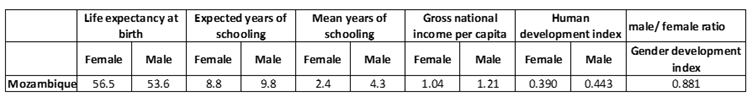
\includegraphics{Figure45.png}

\emph{Source: UNDP Human Development Report 2015}

Extreme poverty and the HIV/AIDS epidemic that has a major impact especially on women and girls have contributed to the precarious situation of women and girls in the country (USAID Gender 2013). Although access to social services has increased, gender and geographical inequalities still persist. Northern and central provinces have less access to education, health services, water, sanitation and social protection. These provincial disparities are reinforced by low per-capita budget allocations. Poorer households are also less likely to access services; for example, antenatal care coverage ranges from 58\% to almost 100\% in the lowest and highest quintile (World Bank 2013). There is a direct correlation between high educational attainment, wealth and greater exposure to the media. The situation is worsened in rural areas, where less than 4\% of women know what internet is (Gillwald et al.~2010). Another challenge for the country's socio-economic development is related to the high illiteracy rate, which for various reasons (especially cultural) affects women (especially in rural areas) more than men (58\% and 30\% respectively) (IOF 2014-2015). Overall, the data surveyed clearly demonstrate that women in Mozambique are disadvantaged in socio-cultural, political and economic terms. This greatly depends on the current gender relations in the country which are highly patriarchal (WLSA 2013). From this perspective of gender inequality, women are highly susceptible to domestic violence and sexual abuse and both contribute to increased poverty, especially among female-headed households (Tvedten, Paulo \& Tuominen, 2009:02).

Studies done in recent years in the country highlight the notion of a ``feminisation of poverty''. That is, on the poverty count, 63\% of female-headed households versus 52\% of male-headed households are poor (CMI 2010). According to the IOF 2014-15, the vast majority of female household heads (76.3\%) are peasants, while among men the proportion of peasants is 55.9\%. The provinces of Gaza and Inhambane are the ones with high numbers of female heads of households, which is justified by the high level of male migration to neighboring South Africa.

\emph{(Source: Mozambique Gender Profile, p.~12-14. Translated from Portuguese)}

\textbf{Gender and Climate Change}

In Mozambique, women and girls are among the groups most affected by poverty. The climate change that cyclically ravages the country runs counter to the government's efforts to eradicate poverty. In this context, climate change has direct impacts on the roles women play in agriculture and food security, in the search for water and firewood for family survival and consequently on the health of family and community members. The impacts of climate change degrade the environment, causing floods and dry land, salinization and contamination of water, soil erosion, destruction of infrastructure, among others. Due to the roles they play in the family, women and girls are forced to travel long distances to find clean water, firewood, etc., taking away time they could dedicate more to their studies and personal development. The delay in the rainy season and the scarcity of rain constrains the woman who has to find alternative means to feed the family, because without rain it is not possible to cultivate the fields. Therefore, the more the weather changes, the greater the workload for women.

\emph{(Source: Strategy and Action Plan on Gender, Environment and Climate Change, p.~2-3. Translated from Portuguese)}

\hypertarget{climate-data-and-information}{%
\section{Climate data and information}\label{climate-data-and-information}}

\hypertarget{communication-education-and-awareness-raising}{%
\section{Communication, education and awareness raising}\label{communication-education-and-awareness-raising}}

\hypertarget{loss-and-damage}{%
\section{Loss and Damage}\label{loss-and-damage}}

\hypertarget{implementation-financing-me}{%
\chapter{Implementation, Financing, M\&E}\label{implementation-financing-me}}

\hypertarget{implementation-strategy}{%
\section{Implementation Strategy}\label{implementation-strategy}}

\hypertarget{financial-resources}{%
\section{Financial Resources}\label{financial-resources}}

\hypertarget{me-and-reporting}{%
\section{M\&E and Reporting}\label{me-and-reporting}}

\hypertarget{annex}{%
\chapter{Annex}\label{annex}}

Bulletin of the Republic, 2018. Water Sector Action Plan For Implementation of the Sustainable Development Goals 2015 - 2030. Official Publication of the Republic of Mozambique. I SERIES - Number 207. National Press of Mozambique.

Bulletin of the Republic, 2019. National Water Resources Plan. Official Publication of the Republic of Mozambique. I SERIES - Number 49. National Press of Mozambique.

Government of The Republic of Mozambique. (2015). Mozambique Intended Nationally Determined Contribution (INDC), 1--12.

Least Developed Countries Expert Group (LDC Expert Group). (2012). National Adaptation Plans: Technical Guidelines for the National Adaptation Plan Process. LDC Expert Group, United Nations Framework Convention on Climate Change (UNFCCC), UNFCCC Secretariat, Bonn, Germany, 148 pp.~

Ministry for the Coordination of Environmental Action (MICOA), 2003. Mozambique Initial National Communication to the United Nations Framework Convention on Climate Change. Government of The Republic of Mozambique.

Ministry for the Coordination of Environmental Action (MICOA), 2010. Strategy and Action Plan on Gender, Environment and Climate Change. Government of The Republic of Mozambique.

Ministry for the Coordination of Environmental Action (MICOA), 2012. National Adaptation Programme of Action (NAPA). Government of The Republic of Mozambique.

Ministry for the Coordination of Environmental Action (MICOA), 2012. National Climate Change Adaptation and Mitigation Strategy. Government of The Republic of Mozambique.

Ministry of Agriculture (MINAG), 2013. National Investment Plan of the Agricultural Sector. Government of The Republic of Mozambique (p.~82). Retrieved from \url{http://www.masa.gov.mz/wp-content/uploads/2018/05/PNISAmoz.pdf}

Ministry of Foreign Affairs of the Netherlands. (2018). Climate Change Profile Mozambique. Ministry of Foreign Affairs of the Netherlands, 20. Retrieved from \url{http://sdwebx.worldbank.org/climateportalb/doc/GFDRRCountryProfiles/wb_gfdrr_climate_change_country_profile}

Ministry of Gender, Children and Social Action (MGCAS), 2016. Mozambique Gender Profile. Government of The Republic of Mozambique.

Ministry of Health (MISAU), 2013. Strategic Plan for the Health Sector PESS 2014-2019. Government of The Republic of Mozambique.

Pereira, I., Mavume A., \& Afonso F., 2011. Disaster Risk Assessment in Mozambique - A Comprehensive Country Situation Analysis. Global Risk Identification Programme (GRIP).

The World Bank, 2019. Disaster Risk Profile Mozambique. Africa Disaster Risk Financing Initiative. The World Bank Group, Washington D.C., July 2019.

The World BanK, 2020. Nutritionally Smart Agriculture in Mozambique (pp.~1--22).

  \bibliography{book.bib,packages.bib}

\end{document}
